%%%%%%%%%%%%%%%%%%%%%%%%%%%%%%%%%%%%%%%%%%%%%%%%%%%%%%%%%%%%%%%%%%%%%%%%%%%%%%%%%
%
% Purpose:  Top level document for \RadiationPressureDesc.  DO NOT EDIT!!!
%
%
%%%%%%%%%%%%%%%%%%%%%%%%%%%%%%%%%%%%%%%%%%%%%%%%%%%%%%%%%%%%%%%%%%%%%%%%%%%%%%%%


\documentclass[twoside,11pt,titlepage]{report}

%
% Bring in the AMS math package
%
\usepackage{amsmath,amssymb,amsfonts,textcomp}

%
% Bring in the common page setup
%
\usepackage{dynenv}

%
% Bring in the common math nomenclature
%
\usepackage{dynmath}

%
% Bring in the model-specific commands
%
\usepackage{radiation_pressure}

%
% Bring in the graphics environment
%
%\usepackage{graphicx}
\usepackage{graphicx}
\usepackage{wrapfig}

%
% Bring in listing environment
%
%\usepackage{paralist}

%
% Bring in the hyper ref environment
%
\usepackage[colorlinks,plainpages=false]{hyperref}
%  keywords for pdfkeywords are separated by commas
\hypersetup{
   pdftitle={\RadiationPressureDesc},
   pdfauthor={\ModelAuthor},
   pdfkeywords={\ModelKeywords},
   pdfsubject={\RadiationPressureDesc}}

\begin{document}

%%%%%%%%%%%%%%%%%%%%%%%%%%%%%%%%%%%
% Front matter
%%%%%%%%%%%%%%%%%%%%%%%%%%%%%%%%%%%
\pagenumbering{roman}

\docid{models/interactions/radiation\_pressure}
\docrev{1.1.1}
\date{\RELEASEMONTH\ \RELEASEYEAR}
\modelname{\RadiationPressureDesc}
\doctype{}
\author{\ModelAuthor}
\managers{
  Robert O. Shelton \\ Project Manager \\
  Michael T. Red \\ Simulation and Graphics Branch Chief \\
  R. Matt Ondler \\ Software, Robotics, and Simulation Division Chief}
\pdfbookmark{Title Page}{titlepage}
\makeDynenvTitlepage

\pdfbookmark{Abstract}{abstract}
%%%%%%%%%%%%%%%%%%%%%%%%%%%%%%%%%%%%%%%%%%%%%%%%%%%%%%%%%%%%%%%%%%%%%%%%%%%%%%%%%
%
% Purpose:  Abstract for the RadiationPressure model
%
%
%%%%%%%%%%%%%%%%%%%%%%%%%%%%%%%%%%%%%%%%%%%%%%%%%%%%%%%%%%%%%%%%%%%%%%%%%%%%%%%%


\begin{abstract}

The magnitude of the radiation pressure force on a spacecraft is generally
small; it has negligible effect on short-duration operations, and is typically
insignificant -- compared to aerodynamic drag and gravitational variabilities --
in Low Earth Orbit.
Nevertheless, the cumulative effect over long-duration operations can produce
a significant perturbation to the vehicle trajectory, and to orbital characteristics.
The \RadiationPressureDesc\ allows for the incorporation of radiative forces
into to \JEODid\ package for state propagation.

\end{abstract}


\pdfbookmark{Contents}{contents}
\tableofcontents
\vfill

\pagebreak

%%%%%%%%%%%%%%%%%%%%%%%%%%%%%%%%%%%
% Main Document Body
%%%%%%%%%%%%%%%%%%%%%%%%%%%%%%%%%%%
\pagenumbering{arabic}


\setcounter{chapter}{0}

%----------------------------------
\chapter{Introduction}\hyperdef{part}{intro}{}\label{ch:intro}
%----------------------------------

\section{Purpose and Objectives of the \RadiationPressureDesc}
%%%%%%%%%%%%%%%%%%%%%%%%%%%%%%%%%%%%%%%%%%%%%%%%%%%%%%%%%%%%%%%%%%%%%%%%%%%%%%%%%
%
% Purpose:  Introduction for the RadiationPressure model.
%
%
%%%%%%%%%%%%%%%%%%%%%%%%%%%%%%%%%%%%%%%%%%%%%%%%%%%%%%%%%%%%%%%%%%%%%%%%%%%%%%%%


%\section{Purpose and Objectives of \RadiationPressureDesc}
% Incorporate the intro paragraph that used to begin this Chapter here.
% This is location of the true introduction where you explain what this model
% does.

The \RadiationPressureDesc\ allows for the incorporation of radiative forces
into the \JEODid\ package for state propagation.

The magnitude of the radiation pressure force on a spacecraft is generally
small, and has negligible effect on short-duration operations.  Nevertheless,
the cumulative effect over long-duration operations can produce significant
perturbations to the orbital characteristics.  The significance of those
perturbations, compared against the perturbations generated by other environmental factors, depends on the specific orbital characteristics.
While the effects of atmospheric drag and
geo-potential terms generally decrease with altitude, the radiation pressure resulting from incident solar
radiation is largely altitude independent, and so becomes increasingly
important at higher altitudes.
For Earth orbits with
semimajor axes around 7000 km (altitude 600 km), radiation pressure effects
become comparable to atmospheric drag effects~\cite{radbib:Milani}.  They dominate
at higher orbits, becoming comparable to the higher order
(\textit{$ l {\geq} 2 $}) geopotential effects at orbit altitudes comparable
to geosynchronous orbits.

Smaller than the direct solar radiation effects, there is also indirect
radiation (or albedo pressure) to consider -- that is, solar radiation reflected
off a third body, such as Earth.
There is also the radiation emitted by the vehicle itself (thermal emission).
For highly reflective surfaces in direct sunlight, this effect is typically two to three orders of magnitude smaller than the effect of
direct solar radiation.  Nevertheless, it becomes significant in several situations:

\begin{itemize}
\item Surfaces that absorb almost all of the incident
radiation have emission forces comparable to the forces resulting from direct solar radiation pressure.
\item Unlit portions of the vehicle (such as on the dark side of the vehicle,
or in the shadow of Earth) obviously have no direct solar pressure, but will continue to experience forces resulting from thermal emission.
\item Deep-space simulations that involve a significant, localized, and
well-insulated heat source, such as a power unit have a particularly strong, localized thermal emission profile, and a solar radiation pressure that is highly dependent upon the distance from Sun.
\end{itemize}

The \RadiationPressureDesc\ in \JEODid\ calculates the effect of the direct
solar radiation pressure, and is structured to allow the easy inclusion of albedo
pressure as a user-specified extension, or in a future release.
With the incorporation of the
\href{file:\JEODHOME/models/interactions/thermal_rider/docs/thermal_rider.pdf}{Thermal
Rider}~\cite{dynenv:THERMALRIDER} model,
the temperature of any surface can be accurately simulated; with this temperature
evolution profile, the \RadiationPressureDesc\ can further model the dynamic effects of
radiation emitted from the vehicle.

The surface of the vehicle can be modeled in two ways.  The default setting is that of a
perfectly symmetric, isothermal sphere.  Alternatively, the
\href{file:\JEODHOME/models/utils/surface_model/docs/surface_model.pdf}{Surface
Model}~\cite{dynenv:SURFACEMODEL}
can be used; this provides the user with the capability of defining any surface
geometry / topology using any combination of materials.

The full Surface Model implementation requires the user to define -- for each material
used in the surface -- the albedo and the fraction of reflected light that is reflected in a
diffuse pattern (as opposed to a specular pattern).  The same can also be specified for the default
surface (which uses only one material over the entire surface).  The default surface also offers the alternative option of specifying the Coefficient of Reflection instead of the albedo and diffuse parameter.  This option IS NOT AVAILABLE for the full Surface Model, because the Coefficient of Reflection is geometry-specific and cannot be easily adapted to the total flexibility in geometry provided by the Surface Model.


\section{Context within JEOD}
The following document is parent to this document:
\begin{itemize}
\item{\href{file:\JEODHOME/docs/JEOD.pdf}
           {\em JSC Engineering Orbital Dynamics}}
			  \cite{dynenv:JEOD}
\end{itemize}

The \RadiationPressureDesc\ forms a component of the \ModelClass\ suite of
models within \JEODid. It is located at
models/\ModelClass/RadiationPressure. It relies on functionality provided as
part of the
\href{file:\JEODHOME/models/interactions/thermal_rider/docs/thermal_rider.pdf}{\em
Thermal-Rider} model~\cite{dynenv:THERMALRIDER} and the
\href{file:\JEODHOME/models/utils/surface_model/docs/surface_model.pdf}{Surface
Model}~\cite{dynenv:SURFACEMODEL}.

\section{Documentation History}
%%%%%%%%%%%%%%%%%%%%%%%%%%%%%%%%%%%%%%%%%%%%%%%%%%%%%%%%%%%%%%%%%%%%%%%%%%%%%%%%%
%
% Purpose:  Change history for document for the RadiationPressure model
%
%
%%%%%%%%%%%%%%%%%%%%%%%%%%%%%%%%%%%%%%%%%%%%%%%%%%%%%%%%%%%%%%%%%%%%%%%%%%%%%%%%


%\section{Documentation History}
%%% Status of this and only this document.  Any date should be
%relevant to when
%%% this document was last updated and mention the reason (release,
%bug fix, etc.)
%%% Mention previous history aka JEOD 1.4-5 heritage in this section.

\begin{tabular}{||l|l|l|l|} \hline
 {\bf Author} & {\bf Date} &  {\bf Revision} & {\bf Description} \\ \hline \hline
 Gary Turner & November, 2009 & 1.0  & JEOD 2.0.0 release \\ \hline
 Gary Turner & April, 2011    & 1.1  & Description of refactoring of model for JEOD 2.2-Alpha2. \\ \hline
 Gary Turner & January, 2012    & 1.1.1  & Change from use of picins to wrapfig.\\ \hline
\end{tabular}



\section{Documentation Organization}
This document is formatted in accordance with the
NASA Software Engineering Requirements Standard~\cite{NASA:SWE}
and is organized into the following chapters:

\begin{description}
%% longer chapter descriptions, more information.

\item[Chapter 1: Introduction] -
This introduction contains four sections: objective and purpose,
context within JEOD, document history, and document organization.

\item[Chapter 2: Product Requirements] -
Describes requirements for the \RadiationPressureDesc.

\item[Chapter 3: Product Specification] -
Describes the underlying theory, architecture, and design of the
\RadiationPressureDesc\ in detail.  It will be organized in
four sections: Conceptual Design, Mathematical Formulations, Detailed
Design, and Version Inventory.

\item[Chapter 4:  User Guide] -
Describes how to use the \RadiationPressureDesc\ in a Trick simulation.  It
is broken into three sections to represent the JEOD
defined user types: Analysts or users of simulations (Analysis),
Integrators or developers of simulations (Integration),
and Model Extenders (Extension).

\item[Chapter 5: Verification and Validation] -
Contains \RadiationPressureDesc\ verification and validation procedures and
results.

\end{description}


%----------------------------------
\chapter{Product Requirements}\hyperdef{part}{reqt}{}\label{ch:reqt}
%----------------------------------

\section{Modeling Requirements}

\requirement{Top-level requirement}
\label{reqt:top_level}
\begin{description}
\item[Requirement:]\ \newline
  This model shall meet the JEOD project requirements specified in
  the \JEODid\
  \hyperref{file:\JEODHOME/docs/JEOD.pdf}{part1}{reqt}{ top-level
  document}~\cite{dynenv:JEOD}.
\item[Rationale:]\ \newline
  This model shall, at a minimum,  meet all external and
  internal requirements
  applied to the \JEODid\ release.
\item[Verification:]\ \newline
  Inspection \vref{inspect:top_level}
\end{description}


%%%%%%%%%%%%%%%%%%%%%%%%%%%%%%%%%%%%%%%%%%%%%%%%%%%%%%%%%%%%%%%%%%%%%%%%%%%%%%%%%
%
% Purpose:  requirements for the RadiationPressure model
%
%
%%%%%%%%%%%%%%%%%%%%%%%%%%%%%%%%%%%%%%%%%%%%%%%%%%%%%%%%%%%%%%%%%%%%%%%%%%%%%%%%

% add text here to describe general model requirements
% text is of the form:
%\requirement{REQUIREMENT DESCRIPTION}
%\label{reqt:REQT_DESC_ABBREVIATED}
%\begin{description}
%  \item[Requirement:]\ \newline
%     <Insert description of requirement>
%  \item[Rationale:]\ \newline
%     <Insert description of rationale>
%  \item[Verification:]\ \newline
%     <Insert description of verification (e.g. "Inspection")>
%\end{description}


\requirement{State Encapsulation}
\label{reqt:stateencapsulation}
\begin{description}
  \item[Requirement:]\ \newline
     The \RadiationPressureDesc\ shall encapsulate the positional state of the vehicle and the
     data necessary to calculate the orientation and position of the vehicle
     with respect to the sun, and planetary bodies.

  \item[Rationale:]\ \newline
     The extent to which radiation pressure acts on the vehicle depends on the
     radiation flux and the orientation of the vehicle with respect to the
     radiation flux.  The magnitude of the radiation flux is a function of
     distance from Sun, and potential shadowing effects of intervening bodies.
     The direction of the force resulting form the interaction depends on the
     relative orientation of the surfaces of the vehicle to the flux vector.

  \item[Verification:]\ \newline
     Inspection \vref{inspect:stateencapsulation}
\end{description}


\requirement{Surface Representation}
\label{reqt:surfacerepresentation}
\begin{description}
  \item[Requirement:]\ \newline
     The \RadiationPressureDesc\ shall offer the capability to model the vehicle surface
as a simple approximation, and as a high-fidelity geometric structure comprising multiple materials.

  \item[Rationale:]\ \newline
     A driving design consideration across the development of
	  \JEODid\ is the ability to do
simple tasks simply.  The inclusion of a radiation pressure model to test the significance of
its inclusion must be a simple task.  Conversely, a simple model may not offer the desired
fidelity, particularly in the situation in which a vehicle is made of multiple materials, or where
there is significant diversion from an isothermal surface.  These capabilities must be provided
for maximal utility of the model.

  \item[Verification:]\ \newline
     Test \vref{test:surfacerepresentation}
\end{description}


\requirement{Temperature Structure}
\label{reqt:temperaturestructure}
\begin{description}
  \item[Requirement:]\ \newline
     The \RadiationPressureDesc\ shall incorporate realistic time-dependent
temperature modeling of its surface.

  \item[Rationale:]\ \newline
     Although thermal emission is typically a relatively small effect of radiation
     pressure modeling, the interaction between the vehicle and radiation is a
     primary contributor to the temperature structure of the vehicle, which may be
     desired by other models.  Furthermore, there are situations in which spatial
     temperature variations do play a significant role in the radiation pressure calculation.

  \item[Verification:]\ \newline
     Tests \vref{test:temperature_integration1} and \vref{test:temperature_integration2}.
\end{description}


\requirement{Albedo Pressure Option}
\label{reqt:albedopressure}
\begin{description}
  \item[Requirement:]\ \newline
     The \RadiationPressureDesc\ shall provide the ability to add  -- at a future time --
     a model to simulate the radiation pressure from sources other than the sun.

  \item[Rationale:]\ \newline
     The solar radiation pressure will typically dominate, but secondary pressure (also known as albedo pressure) from planetary objects is necessary for a complete
     description and more accurate modeling.  These other sources will provide
     a flux that will interact with the vehicle in exactly the same way as the
     solar flux, and should be handled by the same routines.

  \item[Verification:]\ \newline
     Inspection \vref{inspect:albedopressure}.
\end{description}

\requirement{Force and Torque}
\label{reqt:forceandtorque}
\begin{description}
  \item[Requirement:]\ \newline
     The data structures shall include storage of the force and torque on the
     vehicle.

  \item[Rationale:]\ \newline
     The force and torque can be collected within Trick -- or within any other
     simulation engine -- from multiple
     interaction models to provide the overall force and torque on the vehicle
     for integration within the dynamics package for purposes of state
     propagation.

  \item[Verification:]\ \newline
     Inspection \vref{inspect:forceandtorque}.
\end{description}

\section{Functional Requirements}\label{sec:func_reqts}




\requirement{Interaction Modeling}
\label{reqt:functional_interaction}
\begin{description}
  \item[Requirement:]\ \newline
    The model shall be capable of modeling the radiation interaction by appropriate
    combination of the effects of photon
    absorption, diffuse photon reflection (rough surface), specular photon
    reflection (smooth surface), and photon emission (thermal emission).
    \subrequirement{Temperature}\ \newline
      The model shall be capable of independently modeling the temperature of each
      thermally independent
      component (facet) of the overall surface representation.
    \subrequirement{Plate Properties}\ \newline
      Each component of the overall surface representation shall be described
      in terms of its material properties to allow
      the combination of these terms to produce the most physically realistic
      description of the surface-photon interaction.
  \item[Rationale:]\ \newline
    Each type of interaction behaves in such a way to produce a different force
    resulting from the same incident flux.  The relative "weighting" of each
    interaction-type is a function of the material properties, which may not be
    constant over an entire vehicle (e.g. the characteristics of solar array panels may be very
    different from those of a thermal shield).  By assigning the material values to each
    facet, these local variations can be modeled and accounted for.
    The temperature of each plate will be particularly influential on the
    photon
    emission, which varies with temperature to the 4th power.  The sides of the
    vehicle in shadow will tend to be significantly cooler than those that are
    in direct solar illumination, and this spatial temperature variation can be
    modeled on a facet-by-facet basis.
  \item[Verification:]\ \newline
    Tests~\vref{test:Fasd}, \vref{test:temperature_integration1}, and \vref{test:temperature_integration2}
\end{description}



\requirement{Temperature Integration}
\label{reqt:functional_temperature}
\begin{description}
  \item[Requirement:]\ \newline
      The model shall be capable of integrating the time-dependent temperature
      structure in order to maintain an energy balance between thermal energy, and
      net radiative power, derived from consideration of absorption and emission
      processes.
	\item[Rationale:]\ \newline
	  The temperature structure should have physical validity.  Its integration must be independent of the overall state integration because of the influence that temperature variability can have on the state integration.
	\item[Verification:]\ \newline
	  Tests \vref{test:temperature_integration1} and \vref{test:temperature_integration2}.
\end{description}

\requirement{Flux Calculation}
\label{reqt:functional_flux}
\begin{description}
  \item[Requirement:]\ \newline
    The model shall be capable of determining the magnitude and direction of
    the solar flux as a function of the current position with respect to the
    sun.

    \subrequirement{Orientation}\ \newline
      The model shall be capable of calculating the orientation of the vehicle
      with respect to the flux vector.

  \item[Rationale:]\ \newline
    For any given vehicle and vehicle-orientation, the force exerted on the
    vehicle is proportional to the magnitude of the incident flux.
    The interaction between the flux and the vehicle depends on
    the respective angles between the vehicle plates and the flux vector.

  \item[Verification:]\ \newline
    Tests \vref{test:eclipse_annular}, \vref{test:eclipse_transverse}, and \vref{test:orbital_long}.
\end{description}


\requirement{Eclipse Calculation}
\label{reqt:functional_eclipse}
\begin{description}
  \item[Requirement:]\ \newline
    The \RadiationPressureDesc\ shall be capable of determining whether the vehicle is in full
    illumination, in the shadow of a third body, or in a position that is
    partially eclipsed (receiving partial illumination).  In the case of a
    partial eclipse, the model shall be capable of calculating an adjustment to
    the background solar flux to account for that part of the solar disk that is
    not visible.
  \item[Rationale:]\ \newline
    The radiation force depends on the flux, which can be affected by
    intervening objects.  To accurately model the flux, the model must have the
    capability to account for those objects.
  \item[Verification:]\ \newline
    Tests \vref{test:eclipse_annular} and \vref{test:eclipse_transverse}.
\end{description}

\requirement{Eclipsing Bodies}
\label{reqt:eclipsingbody}
\begin{description}
   \item[Requirement:]\ \newline
    The \RadiationPressureDesc\ shall have the capability to calculate the shadowing
    effect of any one intervening body, and the option to extend that capability to
    multiple intervening bodies.
  \item[Rationale:]\ \newline
    There are limited situations where more than one body could
    simultaneously provide significant shadowing, so typically only one object need
    be identified at any particular time.  However, for simulations such
    as an Earth-Moon transit scenario, that object may change (from Earth
    to Moon, for example).

      For future development, it is conceivable that it may be desirable to add the capability
      to monitor the eclipsing of non-planetary third bodies (such as an intervening
      vehicle).  An example of this application would be the temperature modeling of components
      of a larger, composite vehicle, such as International Space Station (ISS).
  \item[Verification:]\ \newline
    Inspection \vref{inspect:eclipsingbody}
\end{description}

\section{Requirements Traceability}\label{sec:traceability}

\begin{longtable}[c]{||p{3in}|p{3in}|}
\caption{Requirements Traceability} \\[6pt]
\hline
{\bf Requirement} & {\bf Inspection and Testing} \\ 
\hline \hline
\endfirsthead
\hline
\endfoot
\caption[]{Requirements Traceability (continued)} \\[6pt]
\hline
{\bf Requirement} & {\bf Inspection and Testing} \\ 
\hline \hline
\endhead
\ref{reqt:top_level} - Top-level Requirements &
  Insp.~\ref{inspect:top_level} \\ \hline

\ref{reqt:stateencapsulation} -  State Encapsulation
& Insp.~\ref{inspect:stateencapsulation} \\ \hline

\ref{reqt:surfacerepresentation} -  Surface Representation
& Test~\ref{test:surfacerepresentation} \\ \hline

\ref{reqt:temperaturestructure} -  Temperature Structure
& Test~\ref{test:temperature_integration1} \\
& Test~\ref{test:temperature_integration2} \\ \hline

\ref{reqt:albedopressure} -  Albedo Pressure Option
& Insp.~\ref{inspect:albedopressure} \\ \hline

\ref{reqt:forceandtorque} -  Force and Torque
& Insp.~\ref{inspect:forceandtorque} \\ \hline

\ref{reqt:functional_interaction} -  Interaction Modeling
& Test~\ref{test:Fasd} \\
& Test~\ref{test:temperature_integration1} \\
& Test~\ref{test:temperature_integration2} \\ \hline

\ref{reqt:functional_temperature} -  Temperature Integration
& Test~\ref{test:temperature_integration1} \\
& Test~\ref{test:temperature_integration2} \\ \hline

\ref{reqt:functional_flux} -  Flux Calculation
& Test~\ref{test:eclipse_annular} \\
& Test~\ref{test:eclipse_transverse} \\
& Test~\ref{test:orbital_long} \\ \hline

\ref{reqt:functional_eclipse} - Eclipse Calculation 
& Test~\ref{test:eclipse_annular} \\
& Test~\ref{test:eclipse_transverse} \\ \hline

\ref{reqt:eclipsingbody} -  Eclipsing Bodies
& Insp.~\ref{inspect:eclipsingbody} \\ \hline

\end{longtable}



%----------------------------------
\chapter{Product Specification}\hyperdef{part}{spec}{}\label{ch:spec}
%----------------------------------

\section{Conceptual Design}
%%%%%%%%%%%%%%%%%%%%%%%%%%%%%%%%%%%%%%%%%%%%%%%%%%%%%%%%%%%%%%%%%%%%%%%%%%%%%%%%%
%
% Purpose:  Conceptual part of Product Spec for the RadiationPressure model
%
%
%%%%%%%%%%%%%%%%%%%%%%%%%%%%%%%%%%%%%%%%%%%%%%%%%%%%%%%%%%%%%%%%%%%%%%%%%%%%%%%%


%\section{Conceptual Design}
This section describes the key concepts found in the \RadiationPressureDesc.  For an
architectural overview, see the \RadiationPressureDesc\
\href{file:refman.pdf} {\em Reference Manual} \cite{radbib:ReferenceManual}.


\subsection{Photon Interaction}

The \RadiationPressureDesc\ models the interaction between a vehicle and the
radiation field in which it is located.  This overall interaction can be
divided and subdivided into four processes, each of which is well understood.

\begin{itemize}
\item{Absorption}\par
When a photon strikes a surface, there is some probability that it will be
absorbed by the surface, thereby raising the energy (observed as a rise in
temperature) of that surface.  The momentum of the photon must also be
absorbed by the surface, since momentum is conserved; this change in momentum
is interpreted as a force, called radiation pressure.
\item{Reflection}\par
There is some probability that the photon will simply bounce off the surface.  While this will not directly affect the material itself, the momentum of the incident photon is absorbed, and the surface will also recoil in response to the momentum that the reflected photon carries in the opposite direction.  There are two distinct types of reflection, \textit{specular} and \textit{diffuse}.  The actual reflection profile of a surface can, in most cases, be modeled to fairly good precision as a combination of these two types, weighted according to the specific material.
\begin{itemize}
\item{Specular}\par
Specular reflection is the type of reflection seen from a smooth surface.  The reflected photon leaves the surface at the same angle as the incident photon.  The result of such reflection is that:
\begin{itemize}\par
\item Parallel to the surface there is no net force, the photon retains its momentum in that direction.
\item Perpendicular to the surface, the photon momentum changes by double the component of the incident photon.
\end{itemize}
\item{Diffuse}\par
Diffuse reflection is the type of reflection seen from dull, matte finishes.  On a microscopic level, the surface is not smooth, and the reflected photon is reflected at some unpredictable angle.  Statistically, diffuse reflection has been well modeled, and we have the Lambertian profile, which forms a cosine density function centered on the normal to the macroscopic surface.  Integrating over that profile produces an effect whereby the entire diffuse reflection profile can be modeled as a single reflection along the normal to the macroscopic surface, but carrying only 2/3 of the photon momentum.  The result of such reflection is that:
\begin{itemize}\par
\item Parallel to the surface the photon momentum changes by the component of the incident photon in that direction.
\item Perpendicular to the surface, the photon momentum changes by the component of the incident photon in that direction, plus 2/3 of the magnitude of the photon momentum.
\end{itemize}
\end{itemize}
\item{Emission}\par
All bodies at temperatures above 0 Kelvin radiate to some extent, with a profile that varies with temperature to the 4th power.  The thermal emission is also modeled with a Lambertian profile, i.e. 2/3 of the power radiated is considered, and it is all emitted normal to the macroscopic surface.
\end{itemize}

An alternative representation considers the vehicle to be an isothermal sphere with some fixed and isotropic combination of the above characteristics.  It is then possible to represent all four interaction methods with a single value, called the Coefficient of Reflection.  It must be realized that this is only relevant to a spherical, isotropic, isothermal surface; the mathematics describing the relation between the four interaction methods and this Coefficient of Reflection are developed in section \reftext{Coefficient of Reflection}{sec:coefficientofreflection}.



\subsection {Radiation Field}
The radiation field is the environment in which the surface is located.  The field has two important effects on the vehicle: it provides energy and momentum.  The energy imbalance (between absorbed and emitted radiation) is critically important when considering the thermal response of a vehicle to the environment.  The momentum imbalance produces a net force and corresponding torque on the vehicle; although this force is typically dominated by aerodynamic uncertainties for low-Earth-orbits, it does become significant for lunar and deep-space missions.

The strength of that field is described by a vector quantity, called the flux, which (somewhat ambiguously) can be defined as the rate at which energy, or momentum, is transmitted through space.  Often, when the intent is to interpret flux as being associated with the momentum, the flux is deliberately identified as the momentum-flux.

Often, there is a dominant source of radiation (typically, that is the sun) that is so overwhelming that any other sources provide negligible effect.  If other sources are to be utilized, it is very important to realize that the flux is not an additive vector.  For example, two bright lights shining at each other do not add to produce zero flux in the middle.  Even in situations where the forces perfectly cancel, it is unlikely that the torques also cancel, and impossible for the thermal responses to cancel, since those are a scalar effect.  Therefore, it is important to consider all sources of flux as being inherently independent, and the radiation field must be considered to be comprised of multiple independent subfields rather than a single accumulated field.

When extending the model to include planetary albedo effects, this concept is particularly important.  While for distant sources it is reasonable to make the assumption that the incident radiation is all parallel, that is an invalid assumption where the source covers a significant solid angle of the environment.  In the latter case, a single source can simultaneously illuminate opposite sides of a single vehicle, and the magnitude of the source itself is a function of the vehicle orientation, as different surfaces `see' more or less of the source.

\subsection {Surface Model}
The interaction is between the radiation field and the surface of the vehicle, so we must have some model of the surface.  This can be modeled simply, using the default spherical isothermal surface, or with greater fidelity using the JEOD Surface Model (first available in JEOD version 2.0.1).

\subsection {Temperature}
The emission from the vehicle depends strongly on surface temperature, and so temperature must be modeled for an accurate representation.  For this, the \RadiationPressureDesc\ relies on the JEOD Thermal-rider model (first available in JEOD version 1.5).

%\section{Mathematical Formulations}
%%%%%%%%%%%%%%%%%%%%%%%%%%%%%%%%%%%%%%%%%%%%%%%%%%%%%%%%%%%%%%%%%%%%%%%%%%%%%%%%%
%
% Purpose:  Mathematical Formulation part of Product Spec for the RadiationPressure model
%
%
%%%%%%%%%%%%%%%%%%%%%%%%%%%%%%%%%%%%%%%%%%%%%%%%%%%%%%%%%%%%%%%%%%%%%%%%%%%%%%%%

\section{Mathematical Formulations}\label{sec:mathformulations}

 \subsection{Reduction of Flux by Intervening Body}\label{ref:shadowcalculator}
 The flux algorithm is qualitatively described in the section
 \textref{calculate\_flux}{ref:calculateflux}.
 The mathematical treatment of flux starts with a trivial inverse-square-law
 application to obtain a raw flux.  A secondary calculation then identifies
 whether that flux is being eclipsed by an intervening body.  This section
 covers that identification, and some of the easier cases.  The intricate
 calculations to determine the fractional eclipse that occurs in a scenario
 in which a part of the solar disk is eclipsed are described in the next
 section (the \textref{Conical Eclipse Calculator}{sec:conicaleclipsecalculator}).

 The \textref{Process Architecture}{sec:processarchitecture}
 contains flow charts (see, in particular, Figures~\ref{fig:flow_calculate_shadow}
 and~\ref{fig:flow_third_body_adjustments}) that assist
 in interpreting the interdependence of these methods.

\subsubsection{Introduction to Problem}
  Suppose that we have a spacecraft orbiting a planet, and that the
  reference frame in which the position of the spacecraft is known is
  arbitrarily oriented, but planet{}-centered.

  Suppose further that the planet is being illuminated by a flux with
  vector \  $\vec{\phi }=\phi \hat{\phi }=\phi \; [\phi _{1},\phi _{2},\phi
  _{3}]$ in that same reference frame, and that the spacecraft is at a
  position  $[x,y,z]$.
  \bigskip
  \bigskip
  \begin{figure}[!ht]
  \begin{center}
    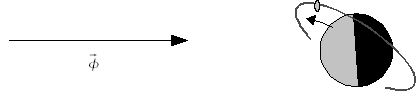
\includegraphics[height=20mm]{figs/shadow/shadow_seeker_fig1.jpg}
    \end{center}
    \caption{Shadowing overview}
    \label{fig:shadow_seeker1}
  \end{figure}

  Define a new coordinate system, \textit{ $\hat{a},\hat{b},\hat{c}$
  }, such that  $\hat{a}$ is oriented with the
  solar flux vector $\vec{\phi}$ for the planet (i.e. from the sun to the
  planet), and $\hat{b}$ and $\hat{c}$ form a
  plane perpendicular to the sun.

  The origin of this coordinate system is concentric with the
  inertial system, so that
  $|\vec{r}_{\mathit{xyz}}|=|\vec{r}_{\mathit{abc}}|$ .
  The new system should be right{}-handed, so that
  $\hat{b}\times \hat{c}=\hat{a}$ .

  The orientation of the \textit{b}{}- and
  \textit{c}{}- axes is arbitrary, and there are an infinity of
  possibilities for such a coordinate system.  However, because we have
  axial symmetry, it is not necessary to define these axes.
  The position vector can, instead, be expressed in terms of two components --
  one parallel, and one perpendicular, to the flux vector.

  \bigskip

  $\vec{r}$ represents the position of the vehicle with respect to the
  shadow body.

  $\vec{d}$ represents the position of the vehicle with respect to the
  sun.

  $r,d$ represent the magnitudes of  $\vec{r},\vec{d}$ respectively.

  \bigskip

  Then the components of the position vector that are parallel and perpendicular
  to the flux vector are (respectively):

  $r_\Vert\ =\ \vec{r}\cdot \hat{\phi }$

  $r_\bot\ =\ \sqrt{r^{2}-r_\Vert^{2}}$

  NOTES
  \begin{itemize}
   \item $r_\Vert \leqslant  0$ places the vehicle on the sunward side of
   the planet.
    In this case, there can be no eclipse.
   \item $r_\Vert > 0$ places the vehicle on the shadow-side of the planet.
    In this case, the determination of whether there is an eclipse depends
    on the value of $r_\bot$.
  \item $r_\bot > 0$ always; the positive square root is taken.
  \end{itemize}


  \bigskip

  \subsubsection{Cylindrical shadowing}\bigskip

  The simplest consideration is one in which the planet casts a
  cylindrical shadow.

  \begin{figure}[!ht]
    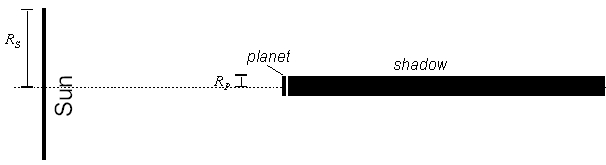
\includegraphics[height=40mm]{figs/shadow/shadow_seeker_fig2.jpg}
    \caption{Cylindrical shadow geometry}
    \label{fig:shadow_seeker2}
  \end{figure}

  \bigskip
  If the spacecraft is in a position such that
  $r_\Vert>0$ and
  $r_\bot<R_{P}$ , then it will be in 100\% shadow.
  \ Otherwise, it will be 100\% illuminated.

  \bigskip

  \clearpage
  \subsubsection{Conical shadowing}\bigskip
  A more complicated scenario is to consider the more realistic conical
  shadow:

  \begin{figure}[!ht]
    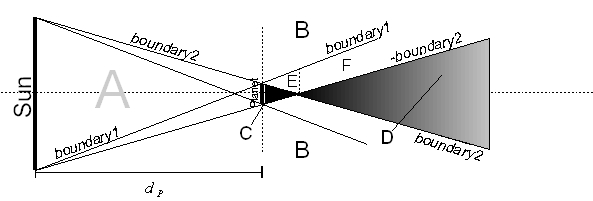
\includegraphics[height=50mm]{figs/shadow/shadow_seeker_fig3.jpg}
    \caption{Conical shadow geometry}
    \label{fig:shadow_seeker3}
  \end{figure}

   \bigskip


   The following sequence of diagrams may help with visualization of the how
   the relative positions of a planet and the sun might change as a vehicle
   moves across the eclipse field.  For this sequence, consider Figure
   \ref{fig:shadow_seeker3} with a vehicle moving from bottom to to through
   regions B-F-D-F-B.
   \begin{itemize}


    \item {}-boundary 1 (B-F): the circle of the planet and
   that of the sun make first contact
   
\includegraphics{figs/shadow/shadow_seeker_fig4.jpg}

    \item boundary 2 (F-D): the planet disk is completely contained
   within the solar disk~~~
   
\includegraphics{figs/shadow/shadow_seeker_fig5.jpg}

    \item {}-boundary2 (D-F): the planet disk begins to leave the
   solar disk~~~~~~~~~~~~~~~~~~~~~~~~
   
\includegraphics{figs/shadow/shadow_seeker_fig6.jpg}

    \item boundary1 (F-B): the two circles separate~~~~~~~~~~~~~~~~~~~~~~~~~~~~~~~~~~
   ~~~~~~~~~~~~~~~~~~
   
\includegraphics{figs/shadow/shadow_seeker_fig7.jpg}

   \end{itemize}
   \bigskip

   The same sequence could also describe a similar path, from top to bottom,
   moving through regions B-E-C-E-B

   \begin{itemize}

   \item boundary 1 (B-E): the circle of the planet and that of the sun make
   first contact

   \item boundary 2 (E-C): the planet disk completely covers the solar disk

   \item {}-boundary2 (C-E): the solar disk starts to emerge from behind the
   planet disk

   \item {}-boundary1 (E-B): the two circles separate

   \end{itemize}


   The two boundaries can be represented as simple lines, $y=mx+b$.
   The gradient for the two boundaries is easily evaluated using the
   distance between the sun and planet, $d_P$.
   \begin{itemize}
    \item boundary1: $\frac{R_P+R_S} {d_P}$
    \item boundary2: $\frac{R_P-R_S} {d_P}$
   \end{itemize}
   The y-intercept for both boundaries is $R_P$.

   Thus, the two boundaries are defined by the relations:
   \begin{itemize}
    \item boundary1: $r_\bot=\left(\frac{R_{P}+R_{S}}{d_{P}}\right)r_\Vert+R_{P}$
    \item boundary2: $r_\bot=\left(\frac{R_{P}-R_{S}}{d_{P}}\right)r_\Vert+R_{P}$
   \end{itemize}


   For the purposes of algebra, let  $b_{1}$  and
    $b_{2}$ represent the values of
   $r_\bot$ that would lie on boundary 1 and boundary
   2, respectively, at some value of  $r_\Vert$ .

   \textbf{Region A} of Figure \ref{fig:shadow_seeker3}, is characterized by
   $r_\Vert<0$.  In this region there will never be any shadow and the full
   disk is counted.


   \textbf{Region B} of Figure \ref{fig:shadow_seeker3} is characterized by
    $r_\Vert>0$ and $r_\bot \geqslant b_{1}$.  In this region, the full disk
    will be counted.

    NOTES:
    \begin{itemize}
     \item $r_\bot>b_{1} \implies r_\bot d_P \geqslant (R_P + R_S)
            r_\Vert + R_P d_P $
    \end{itemize}



   \textbf{Region C} of Figure \ref{fig:shadow_seeker3} is characterized by
   $r_\Vert>0$ and $r_\bot \leqslant b_{2}$.  In this region, the eclipse is
   total; none of the disk will be counted,  $I=0$.

   NOTES:
   \begin{itemize}
    \item $r_\bot<b_{2} \implies r_\bot d_P \leqslant (R_P - R_S) r_\Vert
          + R_P d_P$
    \item Because $R_P < R_S$ (typically) and $r_\bot \geqslant 0$, this becomes
          impossible at large $r_\Vert$, as expected.
   \end{itemize}



   \textbf{Region D} of Figure \ref{fig:shadow_seeker3} is characterized by
   $r_\Vert>0$ and $r_\bot \leqslant -b_{2}$.  In this region, the eclipse will
   be annular, and a function of $r_\Vert$ only (i.e. independent of $r_\bot$).

   NOTES:
   \begin{itemize}
    \item $r_\bot \leqslant -b_{2} \implies r_\bot d_P \leqslant (R_S - R_P)
           r_\Vert - R_P d_P$
    \item For modeling shadowing from a source other than the sun, it could
          be possible to have $R_P > R_S$.  In this case, the left hand side
          of the inequality is positive and the right-hand-side negative-definite.
          The inequality cannot be satisfied and region D is not available.
   \end{itemize}


   In the diagram below, the white circle represents the solar disk, and the
   shaded circle the intervening planetary disk.

   
\includegraphics{figs/shadow/shadow_seeker_fig8.jpg}

   The planetary angular size is  $\frac{2R_{P}}{r}$
   and the solar angular size is  $\frac{2R_{S}}{d}$ .

   The area of the disk is proportional to the square of the angular size;

   hence the planetary disk obscures
   $\left(\frac{R_{P} \cdot d}{R_{S} \cdot r}\right)^{2}$ of the solar disk,

   and the illumination becomes
   \begin{equation*}
   I=1-\left(\frac{R_{P} \cdot d}{R_{S} \cdot r}\right)^{2}
   \end{equation*}

   \bigskip

   \textbf{Region E} of Figure \ref{fig:shadow_seeker3} is characterized by
   $(r_\Vert>0)$ and $(r_\bot>b_{2})$ and $r_\bot<b_{1}$ and
   $\frac{R_P}{r} > \frac{R_S}{d}$.  In this
   region, the eclipse will be partial, transitioning to total.  The magnitude of
   the eclipse effect will be a function of both $r_\Vert$ and $r_\bot$.  The
   resulting illumination will transition from 100\% on
   boundary1 to 0\% on boundary2.

   NOTES:
   \begin{itemize}
    \item Algorithmically, this set of constraints is acheived when the tests
          for regions A-D have failed and $R_P \cdot d > R_S \cdot r$
   \end{itemize}

   In the diagram below, the white circle
   represents the solar disk, and the shaded circle the intervening planetary disk.

   
\includegraphics{figs/shadow/shadow_seeker_fig9.jpg}

   The mathematical treatment of this transition is described in
   subsection \ref{sec:conicaleclipsecalculator}.

   \bigskip

   \textbf{Region F} of Figure \ref{fig:shadow_seeker3} is characterized by
   $(r_\Vert>0)$ and $(r_\bot>b_{2})$ and $r_\bot<b_{1}$ and
   $\frac{R_P}{r} \geqslant \frac{R_S}{d}$.
   In this
   region, the eclipse will be partial, transitioning to annular.  The magnitude of
   the eclipse effect will be a function of both $r_\Vert$ and $r_\bot$.  The
   resulting illumination will transition from 100\% on
   boundary1 to the value determined for region D on (-)boundary2.

   NOTES:
   \begin{itemize}
    \item Algorithmically, this set of constraints completes the set.  It is
          achieved when tests for all other regions have failed.
   \end{itemize}


   
\includegraphics{figs/shadow/shadow_seeker_fig10.jpg}
   The mathematical treatment of this transition is described in
   subsection \ref{sec:conicaleclipsecalculator}.

   \bigskip

   \subsubsection{The flux unit{}-vector}\bigskip

   The direction of the flux acting on the spacecraft in full illumination
   is going to be on a line from the center of the sun reference frame to
   the center of pressure of the spacecraft (or, in the case of a
   representation in terms of multiple facets, the desired vectors
   would be to the center of pressure of each facet).
   The center of pressure of each facet is
   defined relative to the structural reference frame in the Surface Model.

   When the sun is partially obscured, the origin of the flux vector will
   be shifted slightly from the center of the sun to the center of
   radiation, as shown in the diagram below, with the cross representing the
   center of radiation of the partially obscured solar disk.

   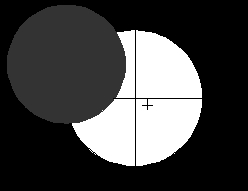
\includegraphics{figs/shadow/shadow_seeker_fig11.jpg}

   If we were to be concerned with the consequential change in direction of the
   flux vector, it would no longer be sufficient to work in the
   axially symmetric, two{}-dimensional system just developed.
   Instead, a full 3{}-dimensional treatment would be required, which would
   add significant computational expense, with minimal impact on the results.
   The radiation pressure is a relatively small force, and the
   effect of the deviation of the direction of the flux vector over such
   small angles is negligible compared to other approximations being made.

   The direction of the flux vector is therefore assumed to be on the
   direction from the center of the sun to some reference point on the
   spacecraft.  Which reference point should be used is not particularly
   relevant for the purposes of determining this direction; using the
   wrong reference point will have even less of an effect than using the
   wrong center of radiation for the source.  Consequently, the same flux
   vector will be used for all of the facets that make up the vehicle.

  \subsection{Conical Eclipse Calculator}\label{sec:conicaleclipsecalculator}

   This subsection describes the method used for calculating the extent of
   shadowing for partial spacecraft shadowing cases, such as would occur in
   in regions E and F of Figure \ref{fig:shadow_seeker3}.

   \bigskip
   \subsubsection{Definitions}


   The front body (the eclipsing body) will be given the subscript
   \textit{1.}

   The rear body (the sun) will be given the subscript \textit{2.}

   The term ``radius'', as used in this description, is not always intended
   to represent the physical radius, but often
   the angular radius, as observed from the point of interest. Reference
   will be made to places where the radius of the planet is larger than
   that of the sun. This does not imply that the planet must be
   physically larger, just that it occupies a larger solid angle due to
   its relative proximity.
   Typically, linear distances are represented by Roman lettering (R, r) and
   angles by Greek lettering ($\theta, \psi, \phi$).
   Ultimately though, we are looking for a fractional area, so both the linear
   and angular sizes will become moot.

   \subsubsection{Introduction}

   Figure \ref{fig:shadow_calc1} shows the area of the shaded subsection of a
   circle, defined by angle  $\theta $ and radius \textit{R}.  It can be
   expressed as
   \begin{equation*}
    A = R^2 (\theta - sin \theta cos \theta)
   \end{equation*}


   \begin{figure}[!ht]
   \begin{center}
    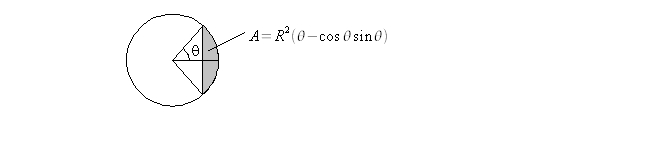
\includegraphics[height=45mm]{figs/shadow/shadow_calculator_fig1.jpg}
    \end{center}
    \caption{The area of the segment of a circle}
    \label{fig:shadow_calc1}
   \end{figure}

   For two intersecting circles, the area can be identified by considering it as
   a sum of two such two circle segments,
   as shown in Figure~\ref{fig:shadow_calc2}~:

   \begin{figure}[!ht]
   \begin{center}
    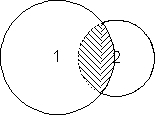
\includegraphics[height=40mm]{figs/shadow/shadow_calculator_fig2.jpg}
    \end{center}
    \caption{The area of overlap of two circles, decomposed into two segments}
    \label{fig:shadow_calc2}
   \end{figure}

   In this diagram, the shaded area on the left
   (
\includegraphics{figs/shadow/shadow_calculator_fig3.jpg})
   is attributed to the circle on the right (labeled 2), while the area on the
   right
   (
\includegraphics{figs/shadow/shadow_calculator_fig4.jpg}), is attributed to
   the circle on the left (labeled 1).
   The total shaded area is then:

   \begin{equation*}
   A\ =\ A_{1}+A_{2}\ =\ {R_{1}}^{2}(\theta _{1}-\cos \theta _{1}\sin
   \theta _{1})+{R_{2}}^{2}(\theta _{2}-\cos \theta _{2}\sin \theta _{2})
   \end{equation*}

   \subsubsection{Direct Computation Method}

   The desired output value is the fraction of this area with respect to the
   area of the solar disk.  Without loss of generality, assign subscript $2$
   to the solar disk and subscript $1$ to the planetary disk.  Use upper-case
   $R_i$ to represent the size of the disk, lower-case $r_i$ to represent the
   distance to the disk, and $\psi_i$ to represent the angular radius of the
   disk.
   \begin{equation*}
     \psi_i = \frac{R_i}{r_i}
   \end{equation*}

   Assign variables to the ratio of angular radii and area:

   \begin{align*}
   \rho &= \frac{\psi_1}{\psi_2} \\
   \alpha &= \frac{A}{\pi R_2^2}
   \end{align*}

   Thus the fractional area $\alpha$ can be expressed in terms of $\rho$ and
   $\theta_i$, independent of $R_i$, $r_i$, and $\psi_i$:
   \begin{equation*}
    \alpha = \frac{1}{\pi} \left( \rho^2(\theta_1 - sin \theta_1 cos\theta_1) +
             \theta_{2}-\cos \theta _{2}\sin \theta _{2} \right)
   \end{equation*}

   To compute the angles $\theta_i$, we start with a triangle with vertices at
   the two disk centers and one of the points of intersection, as shown in Figure
   \ref{fig:shadow_calc_triangle}.

   \begin{figure}[!ht]
   \begin{center}
    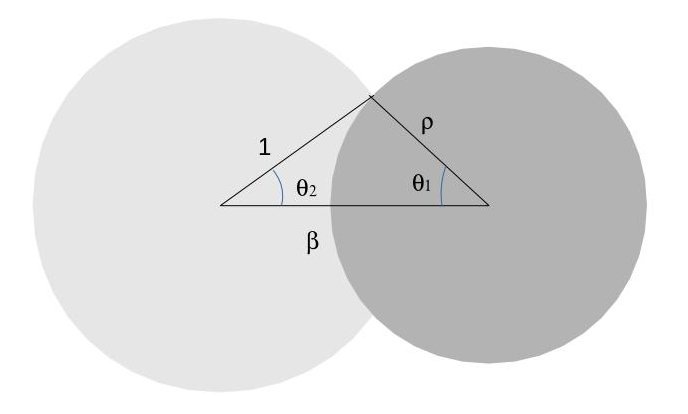
\includegraphics[height=40mm]{figs/shadow/shadow_calculator_fig6.jpg}
    \end{center}
    \caption{The scaled angular sizes of the two disks.}
    \label{fig:shadow_calc_triangle}
   \end{figure}





   The scaled separation between the disk centers is
   \begin{equation*}
     \beta = cos \theta_2 + \rho cos \theta_1
   \end{equation*}
   The perpendicular distance from the line joining the
   centers to the intersection of the two circles is
   \begin{equation*}
     sin \theta_2 = \rho sin \theta_1
   \end{equation*}

   Consequently, the values of $\theta_i$ can be determined:
   \begin{align*}
     \rho^2 cos^2 \theta_1 &= (\beta - cos \theta_2)^2 \\
     \rho^2 cos^2 \theta_1 &= \rho^2 (1 - sin^2 \theta_1) =
                               \rho^2 - sin^2 \theta_2 =
                               \rho^2 -1 + cos^2 \theta_2 \\
     (\beta - cos \theta_2)^2 &= \rho^2 -1 + cos^2 \theta_2  \\
     cos \theta_2 &= \frac{\beta^2 + 1 - \rho^2}{2s} \\
     cos \theta_1 &= \frac{\beta^2 - 1 + \rho^2}{2s \rho}
   \end{align*}

   This still requires an expression for the scaled separation ``distance'',
   $\beta$.  The angle $\phi$  between the two centers can be obtained
   from the cosine rule:

   \begin{equation*}
      d_P^2 = r_1^2 + r_2^2 - 2 r_1 r_2 cos \phi
   \end{equation*}

   where $r_i$ are the linear distances from the vehicle to the respective
   disk-centers, and $d_P$ is the linear distance between disk centers.
   $\beta$ and $\phi$ are related by the angular radius of the solar disk,
   $\psi_2$.

   \begin{equation*}
      \beta = \frac{\phi}{\psi_2} =
      \frac{cos^{-1} \left( \frac{r_1^2 + r_2^2 - d^2}{2 r_1 r_2} \right)}
           {\psi_2}
   \end{equation*}





   Notes:
   \begin{itemize}
   \item This is a cumbersome calculation, requiring
   inverse-trigonometric functions to obtain $\beta$, $\theta_1$ and
   $\theta_2$ and
   2 square-root functions to determine $sin \theta_1$ and $sin \theta_2$.
   \item The calculation $\theta_i = cos^{-1} (cos \theta_i)$ requires that $-1
   \leqslant cos \theta_i \leqslant 1$ but the expressions for
   $cos \theta_i$ have no intrinsic limit protection on them.  However,
   this requirement is handled
   within the overall model algorithm because this computation is only
   reached where $abs(1-\rho) \leqslant \beta \leqslant 1+\rho$; this constraint
   is equivalent to the necessary constraint on the value of $cos \theta_i$.
   \end{itemize}

   An alternative approach provides a very close approximation using a cubic
   polynomial of the separation distance with coefficients that are themselves
   quadratic or cubic polynomials of the ratio of the disk radii.  This
   alternative approach improves speed by a factor of approximately 4.

   \subsubsection{Alternative Representation}

     Using a system of ratios, it is straightforward to identify the extent
     of the eclipse between none and maximum, where maximum occurs when the
     smaller disk is completely covered by the larger disk.
     Note - in the case where
     $R_{2}<R_{1}$, maximum eclipse is total eclipse, whereas when
     $R_{1}<R_{2}$, maximum eclipse will be when the solar disk
     completely encompasses the planetary disk.

   We can introduce $\delta$, $\delta \in [0,1]$  to represent
   the ratio of the
   current extent of the eclipse to its maximum value.

   ${\delta}$ has value \textit{0} when the limbs make first
   contact, and value \textit{1} at second contact (total occlusion).
   It is associated with the linear coverage distance
   $s =  1 + \rho - \beta$ (see  Figure
   \ref{fig:shadow_calc5}) rather than with the occluded area,
   and increases linearly with $s$.\

   Note that the distance between first contact
   and second contact is the diameter of the smaller disk.  Thus
   $s \in [0, min (2R_1,2R_{2})]$.

   \begin{figure}[!ht]
   \begin{center}
    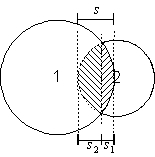
\includegraphics[height=40mm]{figs/shadow/shadow_calculator_fig5.jpg}
    \end{center}
    \caption{Overlap of two circles}
    \label{fig:shadow_calc5}
   \end{figure}

   Thus,
   \begin{equation*}
   s=
   \begin{cases}
     \delta \cdot 2R_{2}     & R_{2}<R_{1} \\
     \delta \cdot 2R_{1}     & R_{1}<R_{2}
   \end{cases}
   \end{equation*}

   In the previous section, we developed an expression for the overlap area
   as a fraction of the area of the solar disk.  Suppose, instead, we had
   developed an expression for the overlap area as a fraction of the smaller
   disk.  Let us label this new fractional area $\alpha_{-}$ and label the
   smaller radius as $R_{-}$.

   Then
   \begin{equation*}
     s = 2 \delta \cdot R_{-}
   \end{equation*}

   Note that the upper bound for $\alpha_{-}$ is independent of the
   relative sizes of the two disks (unlike the upper bound for $\alpha$).
   We always have $0 \leqslant \alpha_{-} \leqslant 1$.

   Now, with the issue associated with relative sizes set aside, we can
   obtain an expression for $\alpha_{-}$ in terms of $\delta$.

   Notice that the final desired result is still $\alpha$, and that must
   depend on whether the solar disk is smaller or larger than the
   planetary disk because we are, after
   all, looking for the fractional covering of the \textit{solar} disk.  This
   dependency can be brought back in after determining a value for
   $\alpha_{-}$:


    \begin{equation*}
     \alpha=
      \begin{cases}
       \alpha_{-} & \rho \geqslant 1 \\
       \rho ^{2}\alpha_{-} & \rho <1
      \end{cases}
    \end{equation*}


   \subsubsection{Polynomial Approximation}

    The quantity $\alpha_{-}$, for all its complexity, is a surprisingly
    well behaved function of \textit{${\delta}$} and can be
    approximated to very high
    precision with a cubic polynomial in \textit{${\delta}$}
    \begin{equation*}
     \alpha _{-}= a_{3}\delta ^{3}+ a_{2}\delta ^{2}+
    a_{1}\delta + a_{0}
    \end{equation*}

    \textbf{Value of $\delta$}

    Recall that $\delta$ is a linear function of the overlap distance, which
    is measured by $r_\bot$.  It starts with value $0$ on boundary $b_1$  at
    first
    contact and climbs to value $1$  at second contact on boundary $b_2$ (or
    $-b_2$, depending on the value of $r_\Vert$).  See Figure
    \ref{fig:shadow_seeker3} for an illustration of these two boundaries.

    Let $b_i$ represent the value of $r_\bot$ on boundary \textit{i}.  Then:

    \begin{equation*}
     \delta =
       \frac{b_1 - r_\bot}{b_1 - \left| b_2 \right|}
    \end{equation*}

    Note that the value of $b_2$ goes negative for $r_\Vert$ greater than
    some critical value, as the planetary disk becomes
    smaller than the solar disk.  To a reasonable approximation, the switch
    in sign occurs when $\rho = 1$ (this is true where $r_\bot = 0$, but
    not quite true off that axis.)

    \begin{equation*}
     \left| b_2 \right| \approx
      \begin{cases}
       b_2 & \rho \geqslant 1 \\
       -b_2 & \rho \leqslant 1
      \end{cases}
    \end{equation*}

    Thus,

    \begin{equation*}
     \delta \approx
      \begin{cases}
       \frac{b_1 - r_\bot}{b_1 - b_2} & \rho \geqslant 1 \\
       \frac{b_1 - r_\bot}{b_1 + b_2} & \rho \leqslant 1
      \end{cases}
    \end{equation*}

   The values $b_i$ can be obtained from geometry (see Figure
   \ref{fig:shadow_seeker3} for an illustration of these two boundaries)
   using simple linear expression $y = mx+b$.

   \begin{align*}
    b_1 &= m_1 r_\Vert + R_P \\
    b_2 &= m_2 r_\Vert + R_P \\
    m_1 &= \frac{R_P + R_S}{d_P} \\
    m_2 &= \frac{R_P - R_S}{d_P}
   \end{align*}

   Thus,
   \begin{equation}
     \delta \approx
      \begin{cases}
       \frac{(R_P - r_\bot) d_P + (R_P + R_S) r_\Vert}{2R_S r_\Vert} & \rho \geqslant 1 \\
       \frac{(R_P - r_\bot) d_P + (R_P + R_S) r_\Vert}{2 R_P( d_P + r_\Vert)} & \rho < 1
      \end{cases}
    \end{equation}


    \textbf{Value of the coefficients $a_i$}

    The coefficients  $a_{i}$ are themselves functions of the radius ratio
    $\rho'$ and can be approximated by quadratic or cubic functions of $\rho'$:

    \begin{equation*}
     \rho' = \frac{R_{-}}{R_{+}}=
      \begin{cases}
       \frac{1}{\rho} & \rho \geqslant 1 \\
       \rho & \rho \leqslant 1
      \end{cases}
    \end{equation*}

    Curve fitting to the analytic solution produces

    $a_{3}(\rho')=0.758656\rho^{'2}-0.0637441\rho' -1.08955$

    $a_{2}(\rho')=-1.2205\rho^{'2} -0.61815\rho' +1.629209$

    $a_{1}(\rho')=0.43723\rho^{'2}-0.529210\rho' +0.473649$

    $a_{0}(\rho')=-0.01242\rho^{'3}-0.0036715\rho^{'2}+0.0150263\rho'
    -0.0078259$

    The approximation is now complete.

    \begin{equation}
    \alpha \approx
    \begin{cases}
        \rho ^{2}\left(
        a_{3}(\rho )\cdot \delta ^{3}+
        a_{2}(\rho )\cdot \delta ^{2}+
        a_{1}(\rho )\cdot \delta +
        a_{0}(\rho )\right)     & \rho <1 \\
        a_{3}\left(\frac{1}{\rho }\right)\cdot \delta ^{3}+
        a_{2}\left(\frac{1}{\rho }\right)\cdot \delta ^{2}+
        a_{1}\left(\frac{1}{\rho }\right)\cdot \delta +
        a_{0}\left(\frac{1}{\rho }\right) & \rho \geqslant 1
    \end{cases}
    \end{equation}

    Figure \ref{fig:shadow_calc7} shows the analytic function and the
    polynomial approximation for values of

    $\rho =30,\ 2,\ 1,\ 0.75,\ 0.5,\ 0.25,\ 0.1$ .

    The analytic solution is shown as a solid line, and
    the approximation as a dotted line for each case.
    The difference between the two lines is small for all cases.


    \begin{figure}[!ht]
      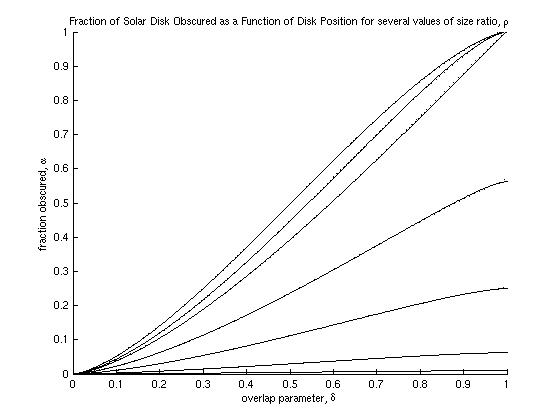
\includegraphics[height=100mm]{figs/shadow/shadow_calculator_fig7.jpg}

      \caption{Comparison of polynomial approximation to analytical solution for
      partial eclipse calculation}
      \label{fig:shadow_calc7}
    \end{figure}

   \subsubsection {Boundary Conditions and Numerical Limitations} \bigskip

    This polynomial approximation should meet certain boundary conditions;
    namely that
    \begin{equation*}
    \delta =0\Rightarrow \alpha =0
    \end{equation*}

    \begin{equation*}
      \delta = 1 \Rightarrow
      \begin{cases}
        \alpha =\rho ^{2}  &  \rho <1 \\
        \alpha =1            &  \rho \geqslant 1
      \end{cases}
    \end{equation*}

    The coefficients given are a result of best{}-fit curve{}-fitting to data
    that intrinsically included the boundary conditions, but the polynomial
    approximation does not explicitly satisfy those conditions.

    For  $\delta =0$ ,  $\alpha \in \left[-8.9\times
    10^{-3},-2.7\times 10^{-3}\right]$ . \ For small values of \textit{
    $\delta $ }, the approximated value of  $\alpha $ is less than the true
    value,
    with a maximum error of 0.89\% when  $\rho =1.0$ .

    For  $\delta =1$ and $\rho <1$,
    $\alpha =\rho ^{2}\left(-0.01242\rho
    ^{3}-0.0283\rho ^{2}+0.04022\rho +1.0054821\right)\ \in
    \ \left[1.005,1.017\right]\times \rho ^{2}$ .

    For  $\delta =1$ and $\rho >1$,
    $\alpha \in \left[1.005,1.017\right]$ ,
    For large values of\textit{ $\delta $ }, the approximated value of
    $\alpha $ is greater than the true value, with a maximum error of 1.7\% when
    $\rho =0.53$ or  $\rho =1.9$.

  \subsection{Response to Flux}\label{sec:mathform_pflux_resp}
    The interaction of matter and radiation is, to say the least, difficult to
    model.  Advances in computer graphics have produced excellent techniques
    for very finely detailed, empirically based, rendering of that interaction,
    but these techniques are typically computationally expensive, and do not
    lend themselves to efficient simulation of orbital dynamics.

    Subsection \ref{sec:mathform_pflux_resp_desc} describes the technique
    used in this model, and subsection
    \ref{sec:mathform_pflux_resp_valid} describes the validation of
    that technique.


    \subsubsection{Treatment of Flux in Calculation of Radiation
    Force}\label{sec:mathform_pflux_resp_desc}


     \begin{wrapfigure}{r}{40mm}
     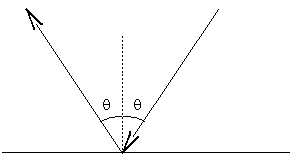
\includegraphics[width = 40mm]{figs/sda/1_sda.jpg}
     \end{wrapfigure}
     \textbf{Specular Reflection:} is the type of reflection observed
     from smooth surfaces, such as mirrors. Incident radiation is
     reflected at the same wavelength and at the same angle so that a
     clear image could, in principle, be obtained.

     \par
     \bigskip
     \bigskip
     \begin{wrapfigure}{r}{40mm}
     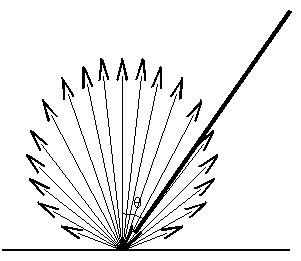
\includegraphics[width = 40mm]{figs/sda/2_sda.jpg}
     \end{wrapfigure}
     %\parpic[r]{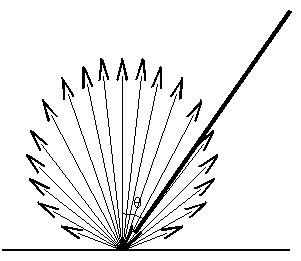
\includegraphics[width = 60mm]{figs/sda/2_sda.jpg}}
     %       \item
     \textbf{Diffuse Reflection} is the type of reflection observed
     from rough surfaces. With a reflection that is totally diffuse,
     all information about the direction of the incident radiation is
     lost, but the radiation is still reflected at the same wavelength
     as the incident radiation.
     \bigskip
     \bigskip
     \bigskip
     \bigskip
     \par
     \textbf{Absorption/Emission}: \textit{absorption} is a process by
     which the incident radiation interacts with the surface structure and
     transfers its energy and momentum to the object. This energy and
     momentum may be partially or entirely \textit{emitted,}
     spontaneously, at some later time, but may be in any direction, and
     at any wavelength. ``Some later time'' may be instantaneous.

     \begin{wrapfigure}{r}{40mm}
     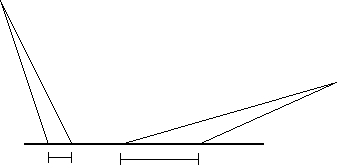
\includegraphics[width = 40mm]{figs/sda/3_sda.jpg}
     \end{wrapfigure}
     \textbf{Lambertian reflection} is a special type of
     diffuse reflection, in which the apparent brightness of the reflected
     light is constant for all viewing angles.  It is clear from the
     accompanying diagram that, when comparing the view
     through a given solid angle, an observer looking at the surface from
     an angle close to
     parallel to the plane (right side of diagram) will see more of the surface
     than an observer
     looking at the surface from an angle close to perpendicular to the plane
     (left side of diagram). If the
     emission were isotropic, the surface would appear brighter the closer
     the observer's line of sight came to being parallel
     with the plane. \ Instead, an emission profile that varies as
     $\cos \theta$ factors in the increased surface area factor
     and produces a uniform brightness for all viewing angles. One of the
     consequences of Lambertian reflection is that of axial symmetry, i.e.
     the reflected light is symmetric about the normal to the plane. For
     the purposes of momentum transfer, the integration over the full range
     of reflected light yields that Lambertian reflection is equivalent to
     absorbing the incident light and emitting 2/3 of it along the normal to
     the plane. Note that this is not true for purposes of calculating
     energy transfer. \par

     The Lambertian profile can also be used to represent the thermal
     emission from the surface; then, for an object in thermal equilibrium,
     the two processes (diffuse reflection and absorption/emission) generate
     the same force (per involved photon of any given energy).
     %\end{itemize}

      \subsubsection{Real Reflection} \bigskip

        Reflection is a complex process involving the interaction of the
        radiation with the electromagnetic potentials created by the
        atomic/molecular structures at and near the surface of the object.
        The effect of these interactions can be empirically measured for
        any given surface, and recorded in a Bidirectional
        Reflectance Distribution Function (BRDF). This
        function provides information on the relative strength of the reflected
        radiation per solid angle, based on the solid{}-angle of incidence.
        Many surfaces have a high degree of symmetry about the normal axis,
        simplifying the 4{}-dimensional BRDF significantly. Even so, assuming
        axial symmetry and therefore requiring only a 2{}-dimensional BRDF for
        each individually oriented exterior surface of a spacecraft is still
        an unrealistic expectation.


      \subsubsection{Overview of Method}
      Photons interacting with matter are typically scattered, or
        absorbed.  We assume that the plates of the spacecraft are
        opaque, so that the scattering process can be treated as
        reflection, with no transmission.
        This model eliminates the computational overhead associated with an
        approximated BRDF, and instead relies on a combination of
        absorption/emission, a Lambertian model of diffuse reflection, and
        specular reflection.  In this approximation, we assume that some
        fixed fraction of the incident radiation is absorbed, and some fraction
        reflected.  Of the reflected radiation, some fraction is
        reflected specularly and some diffusely.  The extent to which
        these three processes contribute to the overall interaction is
        material dependent, and set by the user for each plate.

    \subsubsection{Validation of Radiation Interaction
    Approximations}\label{sec:mathform_pflux_resp_valid}

      To test the validity of this approximation, a series of axially
      symmetric BRDFs were established by constructing a surface from
      pseudo{}-randomly oriented microscopic plates, and assuming specular
      reflection or absorption at each microscopic plate. For each surface (of
      multiple plates), an approximation was attempted that would match the
      observed force characteristics to those of the new model.  For each
      surface, a reasonable model was identified.

      The fundamental consideration is that a photon hits the surface
      and the surface responds in absorbing that momentum, and a photon
      leaves the surface, causing a response in reaction.  Across a
      wide range of materials and angles of incidence, changing the
      relative strengths of the three processes causes differences of only
      a few percent from one another, and a precise determination of the
      weighting values is generally not necessary.

      \subsubsection{The Microscopic Plate Model}\bigskip

        Set up axes such that the surface lies in the x{}-y plane, with the
        z{}-axis defining the surface normal. \ Radiation is incident along the
        x{}-axis, from +x, hitting the surface at the coordinate origin.

        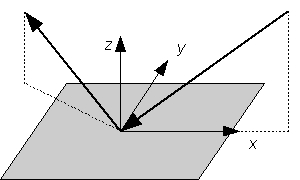
\includegraphics[height=40mm]{figs/sda/4_sda.jpg}

        As each photon is incident on the surface, it hits a random microscopic
        plate, and is reflected accordingly. The orientation of each plate is
        determined by the following algorithm:

        \begin{enumerate}
        \item Rotate the plate about the z{}-axis by some angle  $\theta _{z}$
        with uniform distribution on  $0\leqslant \theta _{z}<\pi $
        \item Rotate the plate about the \textit{rotated} x{}-axis by
        some angle $\theta _{x}$ with normal distribution
        with mean 0 and standard deviation determined by the desired
        ``roughness'' of the surface.
        \end{enumerate}

        Define:

         $\hat{i},\hat{j},\hat{k}$ The unit vectors defined by
        the coordinate system above

         $\hat{p}$ to be the unit vector directed \textit{against }the
         incident radiation

         $\hat{s}$ to be the unit vector associated with the reflected
         radiation, and \textit{x, y, }and\textit{ z }by
         $\hat{s}=x\hat{i}+y\hat{j}+z\hat{k}$

         $\hat{n}$ to be the unit vector normal to the plate

         $\phi $ to be the angle between  $\hat{k}$
         and $\hat{p}$

         $\hat{s}=x\hat{i}+y\hat{j}+z\hat{k}$ can be found in terms of  $\theta
         _{x}$ and  $\theta _{z}$ by the method following.

         \bigskip

         The original reference frame, \textit{O,} is rotated to a new
         reference frame, \textit{O'}, such that the surface normal is
         oriented along $\hat{k}\text{'}$ , the local z{}-axis in
         \textit{O'}.  The axes in
         \textit{O'} can be expressed in terms of the
         angles $\theta _{x}$ and  $\theta _{z}$ so that

         $\begin{gathered}\hat{i}\text{{\textquotesingle}}=\ \cos \theta
         _{z}\hat{i}+\sin \theta _{z}\hat{j}\hfill
         \\\hat{j}\text{{\textquotesingle}}=-\cos \theta _{x}\sin \theta
         _{z}\hat{i}+\cos \theta _{x}\cos \theta _{z}\hat{j}+\sin \theta
         _{x}\hat{k}\hfill \\\hat{k}\text{{\textquotesingle}}=\ \sin \theta
         _{x}\sin \theta _{z}\hat{i}-\sin \theta _{x}\cos \theta
         _{z}\hat{j}+\cos \theta _{x}\hat{k}\hfill \end{gathered}$

         Thus the transformation matrix representing the rotation from
         \textit{O} to \textit{O'} is

         $\left[\begin{matrix}\cos \theta _{z}&\sin \theta _{z}&0\\-\cos
         \theta _{x}\sin \theta _{z}&\cos \theta _{x}\cos \theta _{z}&\sin
         \theta _{x}\\\sin \theta _{x}\sin \theta _{z}&-\sin \theta _{x}\cos
         \theta _{z}&\cos \theta _{x}\end{matrix}\right]$

         \bigskip

         Thus, the vector  $\vec{p}$ can be transformed into \textit{O'}. In
         \textit{O'}, the beam is reflected in the
         local x{}-y plane at the origin, so
         $\hat{s}\text{{\textquotesingle}} = \left[\begin{matrix}s_{1}
         \text{'}\\s_{2}\text{'}\\s_{3}\text{'}\end{matrix} \right] =
         \left[\begin{matrix}-p_{1}\text{'}\\-p_{2}\text{'}\\p_{3}\text{'}
         \end{matrix} \right]$


         Then this can be transformed back into the frame
         \textit{O} by the transpose of the rotation matrix to produce the
         unit vector:

          $\hat{s}=\left[\begin{matrix}\sin \phi (2\sin ^{2}\theta
         _{x}\sin ^{2}\theta _{z}-1)+\cos \phi (2\sin \theta _{x}\cos \theta
         _{x}\sin \theta _{z})\\\sin \phi (-2\sin ^{2}\theta _{x}\sin \theta
         _{z}\cos \theta _{z})+\cos \phi (-2\sin \theta _{x}\cos \theta _{x}\cos
         \theta _{z})\\\sin \phi (2\sin \theta _{x}\cos \theta _{x}\sin \theta
         _{z})+\cos \phi (\cos ^{2}\theta _{x}-\sin ^{2}\theta
         _{x})\end{matrix}\right]$

         \bigskip

         Integrating over all values of $\theta_x$ and $\theta_z$, weighted
         by the respective probability
         functions

         \begin{equation*}
         p(\theta_z) = \frac{1}{\pi} d\theta_z
         \end{equation*}

         \begin{equation*}
         p(\theta_x) = \sqrt {\frac{c}{\pi}} \left( e^{-c {\theta_x}^2} \right) d \theta_x
         \end{equation*}

          produces an expected value

         \begin{equation}
           \langle \hat{s}\rangle =\left[\begin{matrix}-0.5\;\sin \phi
           \;\left(1+e^{-\frac{1}{c}}\right)\\0\\\cos \phi
           \;e^{-\frac{1}{c}}\end{matrix}\right]
           \label{eqn:s_hat_average}
        \end{equation}

         The value \textit{c} in the above expressions is a measure of the
         ``smoothness'' of the surface; a small value \textit{c} tends to a
         uniform distribution on $\theta_x$, indicative of a rough surface,
         while a large value of \textit{c} tends to produce a delta distribution
         on $\theta_x$ (i.e. all parallel to the surface), indicative of a smooth
         surface.

         Note that the average of unit vectors will typically not be a unit
         vector; this value is not a unit vector.

         This value also includes photons reflected ``down'' into the
         surface, which should undergo subsequent reflections until either
         absorbed or reflected out.

         Instead of using this value for the calculation of the force due to
         reflection, the value was numerically simulated by firing 10
         \textsuperscript{6} photons at the surface and tracking each photon
         until it was either absorbed, or reflected out.
         For code validation, this process was changed slightly so that all
         down{}-reflected photons were ignored, and instead re-calculated as
         newly incident photons; these results matched the analytic
         solution to better than 0.5\%.
         The differences observed when the effect of multiple
         reflections is included is seen mostly on the z{}-axis, and
         increases with both the incident angle, $\phi $  and the
         ``smoothness'' factor, \textit{c}.  The results of this
         investigation can be found in the section \textref{Validation of
         Flux-Vehicle Interaction-Model Principles}
         {test:flux_vehicle_interaction}.


         The incremental force added to the surface by a photon is

         \begin{equation*}
         \vec{\mathit{dF}}=\left\{\begin{matrix}\phi _{\gamma
         }\left(-\hat{p}-\hat{s}\right)\ \ \ \ \ \ \ \mathit{reflection}\\\phi
         _{\gamma
         }\left(-\hat{p}-\frac{2}{3}\hat{k}\right)\ \ \
         \mathit{absorption}\end{matrix}\right\}
         \end{equation*}


         and the total force
         \begin{equation}
           \vec{F}=\sum _{i=1}^{i=N}\vec{\mathit{dF}}_{i}
           \label{eqn:force_plate}
         \end{equation}


         The simplifying model used here, that avoids individual photon
         mapping, assumes that some fraction  $\alpha $ is
         reflected form the plane of the whole surface, of which some fraction
         $\delta $ is reflected totally diffusely and
         $1-\delta $ is reflected purely specularly. The
         balance $(1-\alpha )$ is absorbed and re{}-emitted.
         The re{}-emission profile is assumed to be Lambertian, as is the
         diffuse reflection profile. \

         The unit vectors  $\hat{p}$ and
         $\hat{s}$ have the same meaning as before, with

         $\hat{p}=\sin \phi \hat{i}+\cos \phi \hat{k}$

         $\hat{s}=-\sin \phi \hat{i}+\cos \phi \hat{k}$

         The total force then is

\begin{equation*}
         \vec{F}=N\phi _{\gamma }\left(-\hat{p}-\alpha (1-\delta
         )\hat{s}-\frac{2}{3}(1-\alpha (1-\delta ))\hat{k}\right)
\end{equation*}

          Note: under the assumption of thermal equilibrium, there is no
          distinction to be made between the force{}-expression associated with
          diffuse reflection and that with absorption/emission.  The force
          equation can therefore be simplified by saying some fraction
          $\sigma $ is reflected specularly:
          \begin{equation}
            \vec{F}=N\phi
            _{\gamma }\left(\hat{i}(\sin \phi )(\sigma -1)+\hat{k}\left((\sigma
            -1)\left(\frac{2}{3}-\cos \phi \right)-2\cos \phi \right)\right)
            \label{eqn:force_model}
          \end{equation}

          The value $\sigma $ can now be found as the
          value that minimizes the error between the two forces (equations
          \ref{eqn:force_plate} and \ref{eqn:force_model})

          The value $\alpha $ can be found from a count
          of the number of absorbed and reflected photons in the microscopic
          plate model,

          \begin{equation*}
          \alpha =\frac{n_{\mathit{reflected}}}{n_{\mathit{photons}}}.
          \end{equation*}

          The value $\delta $ can be found from $\alpha $ and $\sigma $ .

          A validation of this model can be found in section
          \textref{Validation of Flux-Vehicle Interaction-Model Principles}
          {test:flux_vehicle_interaction}.

  \subsection{Response of Temperature and Thermal Emission to Incident Flux}
  \label{sec:mathform_temp_resp}

    \subsubsection{Temperature Variation}
      Without a source of incident energy, the object should cool by
      radiation, according to

      \begin{equation}
        C\frac{\mathit{dT}}{\mathit{dt}}=-\epsilon A\sigma T^{4}
      \end{equation}

      where \textit{C} represents the heat capacity,
      $\epsilon $ the emissivity ,  $\alpha $ the albedo,
      \textit{ A} the emitting area,
      $\sigma $ the Stefan{}-Boltzmann constant, and
      \textit{T} the temperature.

      $\alpha$ and $\epsilon$ are surface dependent values, and must
      be included as part of the plate model.

      The analytic solution to this expression is

      \begin{equation}
        T(t)=\frac{T_{0}}{\sqrt[{3}]{1+3\left(\frac{\epsilon \sigma
        A}{C}\right)\;(T_{0})^{3}\;t}}
      \end{equation}

      with  $T(0)=T_{0}$

      The simulation is tested against this analytic result in section
      \vref{test:temperature}.

      There is no closed{}-form analytic solution for the case of an
      illuminated plate.

      For the temperature response under illumination, we first consider
      the variation of the force due to thermal emission, described  in
      the next subsection.

    \subsubsection{Variation of Force due to Thermal Emission}

      The force due to emission can be calculated from the magnitude of the
      momentum carried away with the
      emission in the direction of that emission, which is given by
      \begin{equation*}
      \frac{1}{c}\frac{\mathit{dE}}{\mathit{dt}},
      \end{equation*}

      Thus,
      \begin{equation}
        \vec{F}=\frac{2}{3}\frac{1}{c}\frac{\mathit{dE}}{\mathit{dt}}(-\hat{n})
      \end{equation}

      with \textit{c} representing the speed of light,
      \textit{E} the energy, and  $\hat{n}$ the normal to the plate surface.


      Due to symmetry, the total vector momentum emitted will be in the
      direction of the normal vector. Because the emission is not
      unidirectional, there will be components of the emission with
      opposing momentum vectors oriented in the plane of the
      surface; consequently, the magnitude of the \textit{net}
      momentum emission will not be equal to the ratio of the
      \textit{total} energy emission to the speed
      of light.  Instead, we have to assume an emission profile; in
      this model, we assume a Lambertian profile for which the necessary factor
      to account for the difference is 2/3 (see subsection
      \ref{sec:mathform_pflux_resp_desc} for description
      of the Lambertian profile).

      The force on the plate is, of course, in the opposite direction to the
      emission.

      Then, continuing the assumption that the plate is not
      illuminated, the force exerted on the plate by its emission is

      \begin{equation}
         F=\frac{2\epsilon \;\sigma
         \;A\;{T_{0}}^{4}}{3c}\left(1+\frac{3\epsilon \;\sigma
         \;A}{C}\;(T_{0})^{3}t\right)^{-{\frac{4}{3}}}
      \end{equation}

      It should be recognized that the values of \textit{t} for the force and
      for the temperature are necessarily different due to the discretization
      of time in the simulation. The analytic expressions are valid for any
      particular time, \textit{t}, and this is sufficient for the
      temperature.  However, the force will be converted to acceleration,
      then integrated to provide velocity and position increments.
      Using the value of the force at either the beginning or end of a
      timestep, for the entire integration leads to errors; a more accurate
      representation would be to use some midpoint value. Instead, the
      force is
      calculated at time \textit{t} for the timestep from \textit{t
      }to\textit{ t+}\textit{${\Delta}$}\textit{t. } A closer
      approximation for the calculated force would be:

      \begin{equation}
        F(t\rightarrow t+\Delta t)\approx \frac{2\epsilon \;\sigma
        \;A\;{T_{0}}^{4}}{3c}\left(1+\frac{3\epsilon \;\sigma
        \;A}{C}\;(T_{0})^{3}\left(t+\frac{\Delta
        t}{2}\right)\right)^{-{\frac{4}{3}}}
      \end{equation}

      The simulation handles this problem by first integrating the temperature
      over the timestep using a Runge{}-Kutte 4\textsuperscript{th} order
      algorithm:

      The intermediate temperature deltas, $I_{1}, I_{2}, I_{3}, and I_{4}$
      are calculated by

      $I_{1}={\frac{\Delta t}{C}}\left( {\Pi-\epsilon A \sigma {T_{i}}^{4}}
      \right)$

      $I_{2}={\frac{\Delta t}{C}}\left( {\Pi-\epsilon A \sigma \left( {
      T_{i} + I_{1}/2} \right) ^{4} } \right)$

      $I_{3}={\frac{\Delta t}{C}}\left( {\Pi-\epsilon A \sigma \left( {
      T_{i} + I_{2}/2} \right) ^{4} } \right)$

      $I_{4}={\frac{\Delta t}{C}}\left( {\Pi-\epsilon A \sigma \left( {
      T_{i} + I_{3}} \right) ^{4} } \right)$

      and averaged to give

      $T_{i+1} = T_{i} + \left( \frac {I_{1}+2I_{2}+2I_{3}+I_{4}}{6}
      \right)$

      where
      \begin{itemize}
        \item{}$\Delta t$ is the timestep;
        \item{}$\sigma$ is the Stefan-Boltzmann constant; and
        \item{}C is the heat capacity,
        \item{}$\Pi$ is the power absorption rate from all sources,
        \item{}$\epsilon$ is the emissivity,
        \item{}A is the area, and
        \item{}$T_{i}$ is the starting temperature of the plate.
      \end{itemize}

      Then, using an energy balance,

      $C \Delta T = \left( \Pi - \xi \right) \Delta t$

      the rate at which energy is emitted, $\xi$, is
      calculated based on the temperature change and the energy absorbed
      during that timestep.

      This emitted energy is converted into a
      momentum, and multiplied by the 2/3 that results from the integration
      over the Lambertian emission profile to give a time{}-averaged
      force, valid over the entire timestep.

      \begin{equation}
        \langle \vec F \rangle = \frac{2}{3c}
        \left( \frac{C \Delta T}{\Delta t} -\Pi \right) \hat n
      \end{equation}


      Consequently, the routine
      \textit{thermal\_integrator} calculates the value corresponding to the
      energy balance over the timestep that is in turn used in the
      calculation of the emission force by routine
      \textit{radiation\_pressure.}



\subsection{Coefficient of Reflection}\label{sec:coefficientofreflection}

When using the single isotropic, isothermal, spherical, default surface,
there is the option to use a Coefficient of Reflection rather than the
combination of albedo and diffuse parameters.  This section describes how
that coefficient is used in the more general framework.

The concept of the Coefficient of Reflection is that the vehicle can be
modeled as a single, perfectly absorbing, flat plate, with some
\textit{effective area, A'} that is always oriented perpendicular to the flux
vector (i.e. its normal vector and the flux vector are anti-parallel).  To
obtain a constant area requires that the vehicle be modeled as a sphere,
so that its orientation cannot affect its projected area.

The physical dimensions of the vehicle can then be modeled with a single
parameter, the radius, \textit{R}.  The cross-sectional area that the
vehicle projects perpendicular to the flux vector is then $\pi R^2$.

In general, $A' \neq \pi R^2$.  The difference is due to the difference
between the reflective characteristics of the real surface and the assumed
perfect absorption of the simple surface.  That difference is modeled as
the Coefficient of Reflection, $C_R$:

\begin{equation*}
A' = C_R \pi R^2
\end{equation*}

Just as with the regular surface, developed in the Surface Model, the
simple surface can be considered to interact with the radiation field
through absorption, specular reflection, and diffuse reflection.

\subsubsection{Absorption}
The projected area absorbs everything that is incident upon it; the
projected area and
effective area are identical.  $C_R = 1.0$

\subsubsection{Specular Reflection}
Figure \ref{fig:defaultsurfacespecular} shows a representation of a
sphere, illuminated from the right, with three light rays added showing
the paths due to specular reflection.

\begin{figure}[!ht]
\begin{center}
    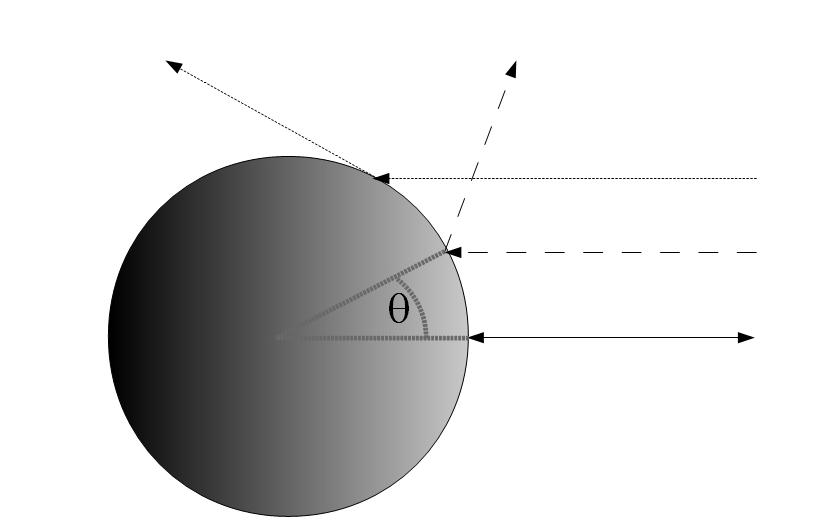
\includegraphics[height=60mm]{figs/def_surf/specular.jpg}
    \end{center}
    \caption{Light Rays Incident on a Specular Spherical Surface}
    \label{fig:defaultsurfacespecular}
  \end{figure}

One ray is reflected stright back, one is reflected at an angle close
to perpendicular to its incident path, and another is deflected very
little from its incident path.  For a photon hitting the surface at a
point that subtends some angle $\theta$ from the flux vector, the
reflected ray will be at angle $2 \theta$.  The momentum change of
the photon (defining the x-axis as being anti-parallel to the flux
vector) is then

\begin{equation*}
\Delta \vec{p} = p(\hat{i} + \cos 2\theta \hat{i} + \sin 2\theta \hat j)
\end{equation*}

where $p$ is the magnitude of the momentum of the photon.

Assuming that the sphere is uniformly illuminated (at least across
the illuminated side) leads to the argument that, by symmetry, the
forces off the x-axis will cancel to zero.

To obtain the force along the x-axis, consider dividing the sphere
into concentric rings, centered about $\theta = 0$.  For a small
range, $d\theta$, there will be a ring of elemental area
$(2 \pi R \sin \theta)(R d\theta)$.  This elemental area will
project, perpendicular to the flux vector, an area
$(2 \pi R^2 \sin \theta d \theta) \cos \theta$.

Therefore, the fraction of the projected disk resulting from the
sphere at some angle $\theta$ is

\begin{equation*}
\delta(\theta) = 2 \sin \theta \cos \theta d \theta = \sin 2 \theta d \theta
\end{equation*}

This is the fraction of the total flux that is incident at any
particular angle $\theta$.

The force due to specular reflection is then

\begin{equation*}
\vec F = \vec \phi \pi R^2 \int_{0}^{\pi/2} (1 + \cos 2\theta) sin 2\theta d\theta
\end{equation*}

where $\vec \phi$ is the momentum flux vector ($N cdot m^{-2}$).

The somewhat surprising result of this integration is that

\begin{equation*}
\vec F = - \vec \phi \pi R^2
\end{equation*}

i.e., the specular sphere behaves exactly the same as a perfectly
absorbing sphere, and therefore has $C_R = 1.0$.

While this may not be expected, it is logical with further consideration.
The photons incident very close to the edge of the sphere will
continue almost unaffected, resulting in minimal force on the
sphere.  Conversely, the photons incident near the center will
be reflected back on the same path, resulting in twice the force
that they would produce if absorbed.  Those incident with
$\theta = 45 ^o$ will exert exactly the same force (along
the x-axis) on the sphere as they would exert if absorbed.
Therefore, the photons hitting inside 45 degrees exert additional
force, those outside 45 degrees exert less force, with nice symmetry.
Integrating the projected area for $0 \leqslant \theta < 45^o$ and
for $45 < \theta \leqslant 90^o$ yields the same value; the deficit
resulting from those photons outside the 45 degree circle balances
with the excess from those inside the circle.

\subsubsection{Diffuse Reflection}
The diffuse reflection is handled using a Lambertian profile and the
same mathematical methods as in the previous section.

\begin{equation*}
\vec F = \vec \phi \pi R^2 \int_{0}^{\pi/2} \left(1 + \frac{2}{3} \cos \theta \right) sin 2\theta d\theta = \frac{13}{9} \vec \phi \pi R^2
\end{equation*}

i.e., the diffuse sphere produces a larger force than would a specular
or absorbing sphere of the same size, and has $C_R = \frac{13}{9}$.

\subsubsection{Composite Surface}
Combining the three processes together yields

\begin{equation}
C_R = (1-\alpha) + \alpha(1-\delta) + \frac{13}{9} \alpha \delta  = 1 + \frac{4}{9} \alpha \delta \in[1.0,1.444]
\end{equation}
where $\alpha$ is the albedo and $\delta$ is the diffuse parameter.

Note that there is a one-to-many relation between the values of
$C_R$ and the values of $\alpha, \delta$.

The code continues to use $\alpha$ and $\delta$; when a user
specifies a coefficient, it is converted into

$\alpha =\frac{9}{4} (C_R - 1)$ and $\delta = 1 $

%\section{Detailed Design}

%%%%%%%%%%%%%%%%%%%%%%%%%%%%%%%%%%%%%%%%%%%%%%%%%%%%%%%%%%%%%%%%%%%%%%%%%%%%%%%%%
%
% Purpose:  Detailed part of Product Spec for the RadiationPressure model
%
%
%%%%%%%%%%%%%%%%%%%%%%%%%%%%%%%%%%%%%%%%%%%%%%%%%%%%%%%%%%%%%%%%%%%%%%%%%%%%%%%%

\section{Detailed Design}

This section is divided into 3 parts:


{\begin{itemize}
\item A process flow-through description, or process architecture, of the
sequence in which the
various functions are called, and the interaction between the objects.
\item An alphabetized list of the objects that comprise the
 \RadiationPressureDesc\
with reference to the parent class where appropriate, and description
of the functions contained within the object.
\item A description of the external data files used by the objects.
\end{itemize}}

Further, the
\href{file:refman.pdf} {\em Reference Manual} \cite{radbib:ReferenceManual}
contains a
structural overview of the \RadiationPressureDesc.

\subsection{Process Architecture}\label{sec:processarchitecture}
This section describes the flow from function to function.  The
operation of each function is described under its object in the section
 \reftext{Functional Design}{sec:FunctionalDesign}.



\clearpage
\subsubsection{Flow charts of the \RadiationPressureDesc\ architecture}
\begin{figure}[!ht]
  \ \newline \ \newline
  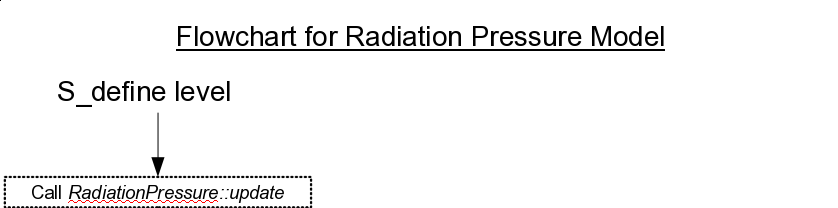
\includegraphics[width = 6 in]{figs/flowchart/flow_top_level.png}
  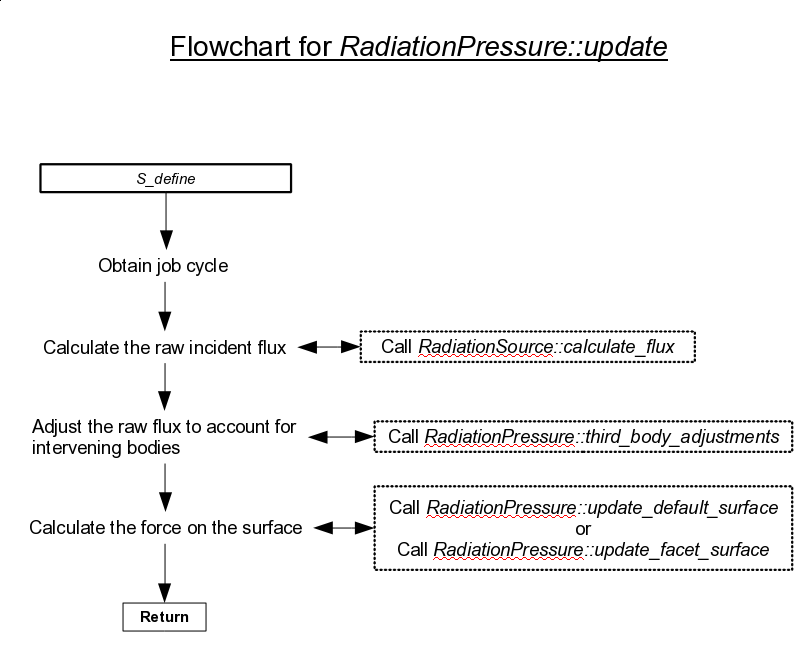
\includegraphics[width = 6 in]{figs/flowchart/flow_update.png}
  \caption{Flowcharts for Radiation Pressure Model }
  \label{fig:flow_update}
\end{figure}

Links: \newline
\textref{RadiationSource::calculate\_flux}{fig:flow_calculate_flux} \newline
\textref{RadiationPressure::third\_body\_adjustments}{fig:flow_third_body_adjustments} \newline\textref{RadiationPressure::update\_default\_surface}{fig:flow_update_default_surface} \newline
\textref{RadiationPressure::update\_facet\_surface}{fig:flow_update_facet_surface}
\clearpage

\begin{figure}[!ht]
  \ \newline \ \newline
  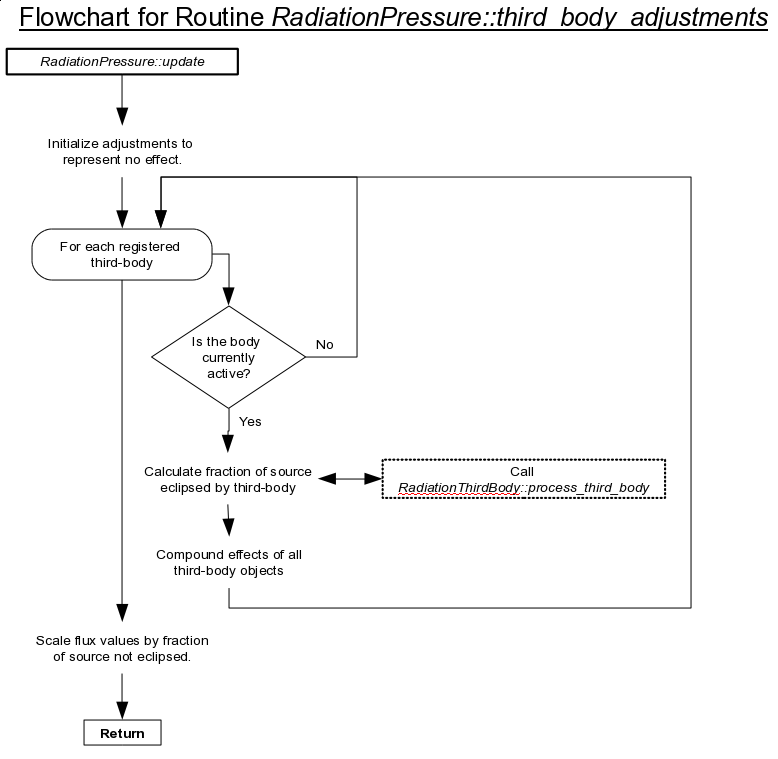
\includegraphics[width = 6 in]{figs/flowchart/flow_third_body_adjustments.png}
  \caption{Flowcharts for Radiation Pressure Model (continued) }
  \label{fig:flow_third_body_adjustments}
\end{figure}

Links: \newline
\textref{RadiationPressure::update}{fig:flow_update}\newline
\textref{RadiationThirdBody::process\_third\_body}{fig:flow_process_third_body} \newline
\clearpage


\begin{figure}[!ht]
  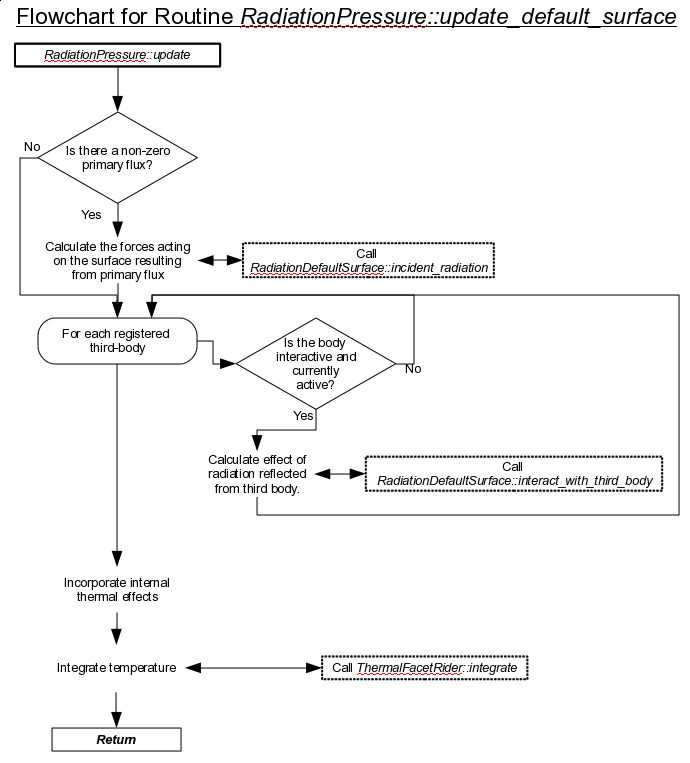
\includegraphics[width = 6 in]{figs/flowchart/flow_update_default_surface.png}
  \caption{Flowcharts for class RadiationPressure (continued)}
  \label{fig:flow_update_default_surface}
\end{figure}
Links: \newline
\textref{RadiationPressure::update}{fig:flow_update}\newline
\textref{RadiationDefaultSurface::incident\_radiation}{fig:flow_default_incident_radiation} \newline
\textref{RadiationDefaultSurface::interact\_with\_third\_body}{fig:flow_default_interact_with_third_body} \newline
\textref{ThermalFacetRider::integrate}{fig:flow_facet_thermal_integrate}\newline
\clearpage



\begin{figure}[!ht]
  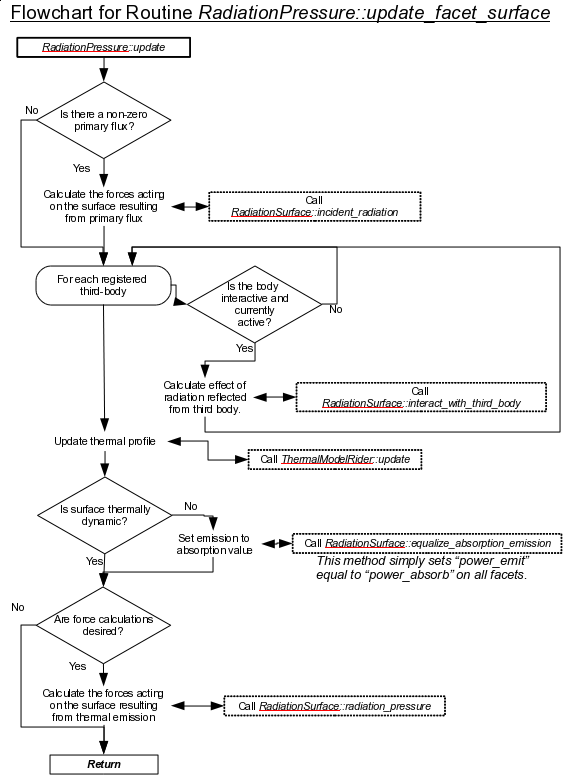
\includegraphics[width = 5 in]{figs/flowchart/flow_update_facet_surface.png}
  \caption{Flowcharts for class RadiationPressure (continued)}
  \label{fig:flow_update_facet_surface}
\end{figure}
Links: \newline
\textref{RadiationPressure::update}{fig:flow_update}\newline
\textref{RadiationSurface::incident\_radiation}{fig:flow_incident_radiation}\newline
\textref{RadiationSurface::interact\_with\_third\_body}{fig:flow_interact_with_third_body} \newline
\textref{ThermalModelRider::update}{fig:flow_thermal_update}\newline
\textref{RadiationSurface::radiation\_pressure}{fig:flow_radiation_pressure}
\clearpage



\begin{figure}[!ht]
  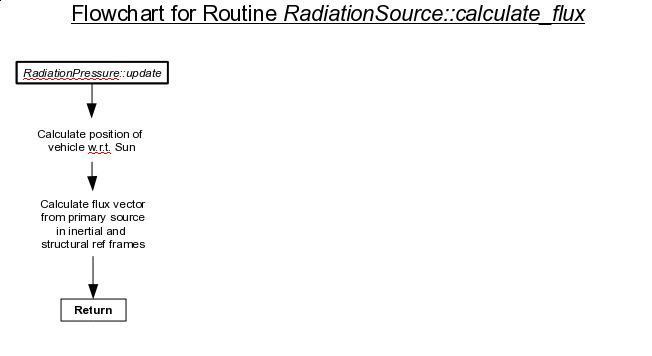
\includegraphics[width = 6 in]{figs/flowchart/flow_calculate_flux.png}
  \caption{Flowchart for class RadiationSource }
  \label{fig:flow_calculate_flux}
\end{figure}
Links: \newline
\textref{RadiationPressure::update}{fig:flow_update}\newline
\clearpage


\begin{figure}[!ht]
  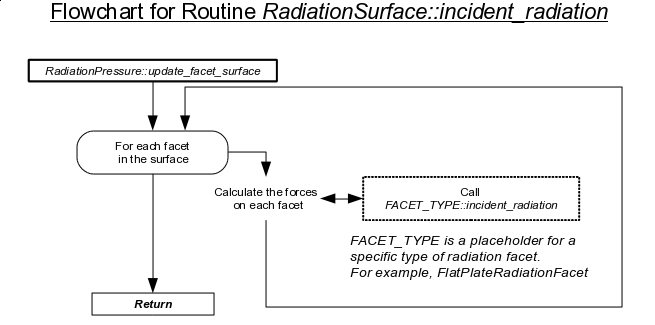
\includegraphics[width = 6 in]{figs/flowchart/flow_incident_radiation.png}
  \label{fig:flow_incident_radiation}
  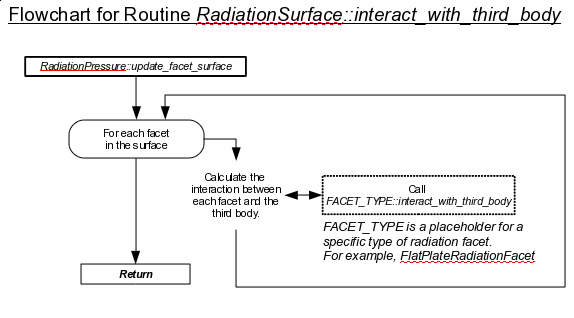
\includegraphics[width = 6 in]{figs/flowchart/flow_interact_with_third_body.png}
  \label{fig:flow_interact_with_third_body}
  \caption{Flowcharts for class RadiationSurface }
\end{figure}
Links: \newline
\textref{RadiationPressure::update\_facet\_surface}{fig:flow_update_facet_surface}\newline
\textref{FlatPlateRadiationFacet::incident\_radiation}{fig:flow_FP_incident_radiation}\newline
\textref{FlatPlateRadiationFacet::interact\_with\_third\_body}{fig:flow_FP_interact_with_third_body}\newline
\clearpage

\begin{figure}[!ht]
  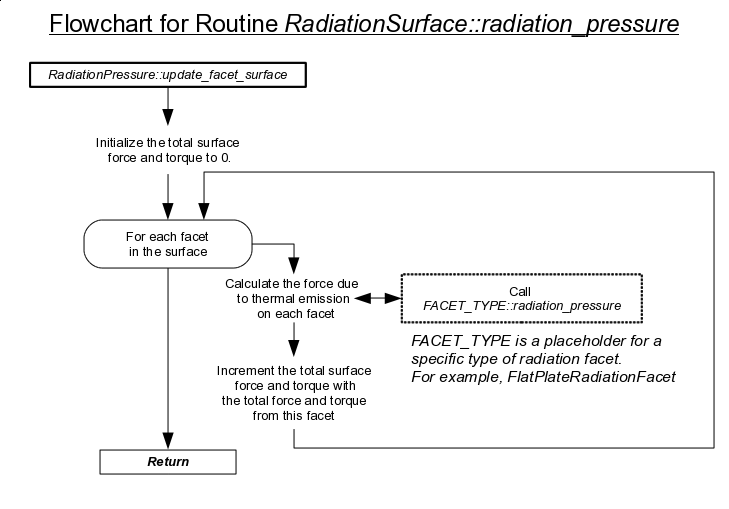
\includegraphics[width = 6 in]{figs/flowchart/flow_radiation_pressure.png}
  \label{fig:flow_radiation_pressure}
  \caption{Flowcharts for class RadiationSurface (continued) }
  
\end{figure}
Links: \newline
\textref{RadiationPressure::update\_facet\_surface}{fig:flow_update_facet_surface}\newline
\textref{FlatPlateRadiationFacet::radiation\_pressure}{fig:flow_FP_radiation_pressure}\newline
\clearpage

\begin{figure}[!ht]
  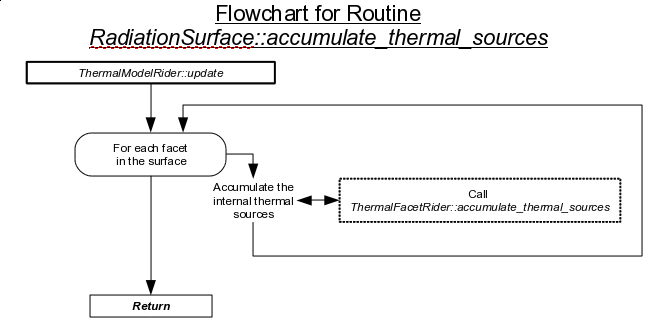
\includegraphics[width = 6 in]{figs/flowchart/flow_accumulate_thermal_sources.png}
  \label{fig:flow_accumulate_thermal_sources}
  
  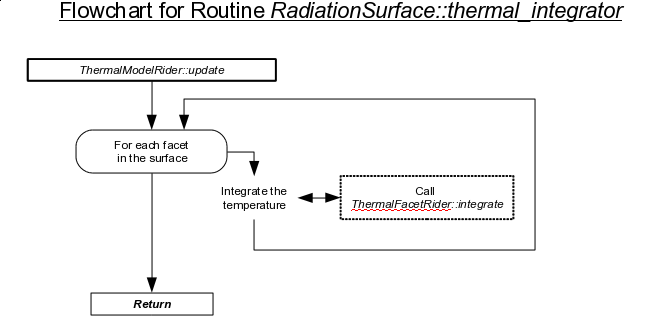
\includegraphics[width = 6 in]{figs/flowchart/flow_thermal_integrator.png}
  \label{fig:flow_thermal_integrator}
  \caption{Flowcharts for class RadiationSurface (continued) }
  
\end{figure}
Links: \newline
\textref{ThermalModelRider::update}{fig:flow_update}\newline
\textref{ThermalFacetRider::accumulate\_thermal\_sources}{fig:flow_facet_accumulate_thermal_sources}\newline
\textref{ThermalFacetRider::integrate}{fig:flow_facet_thermal_integrate}\newline
\clearpage



\begin{figure}[!ht]
  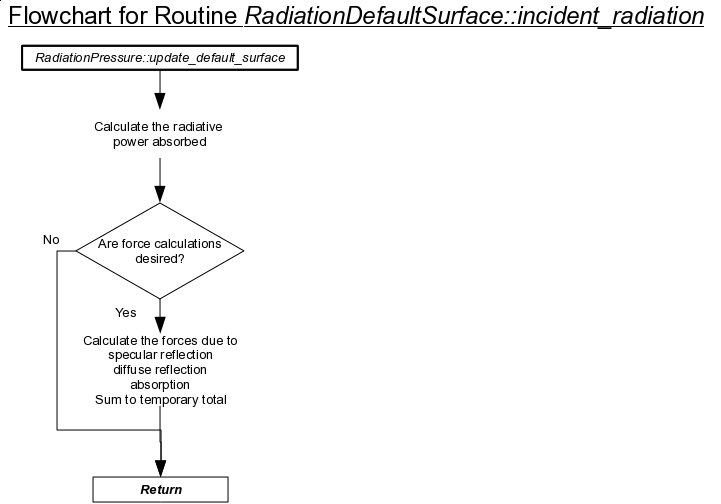
\includegraphics[width = 6 in]{figs/flowchart/flow_default_incident_radiation.png}
  \caption{Flowchart for class RadiationDefaultSurface }
  \label{fig:flow_default_incident_radiation}
\end{figure}
Links: \newline
\textref{RadiationPressure::update\_default\_surface}{fig:flow_update_default_surface}
\clearpage

\begin{figure}[!ht]
  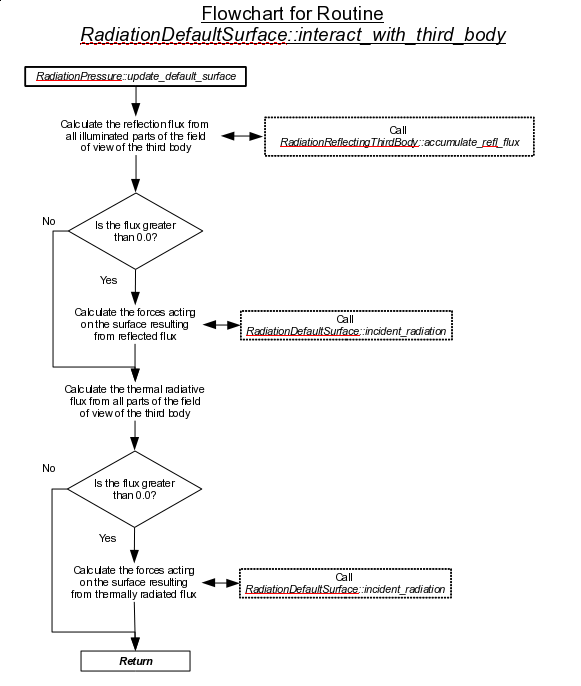
\includegraphics[width = 6 in]{figs/flowchart/flow_default_interact_with_third_body.png}
  \caption{Flowchart for class RadiationDefaultSurface (continued) }
  \label{fig:flow_default_interact_with_third_body}
\end{figure}
Links: \newline
\textref{RadiationPressure::update\_default\_surface}{fig:flow_update_default_surface}\newline
\textit{RadiationReflectingThirdBody::accumulate\_refl\_flux}(not implemented) \newline
\textref{RadiationDefaultSurface::incident\_radiation}{fig:flow_default_incident_radiation}\newline
\textit{RadiationReflectingThirdBody::accumulate\_rad\_flux}(not implemented) \newline
\clearpage


\begin{figure}[!ht]
  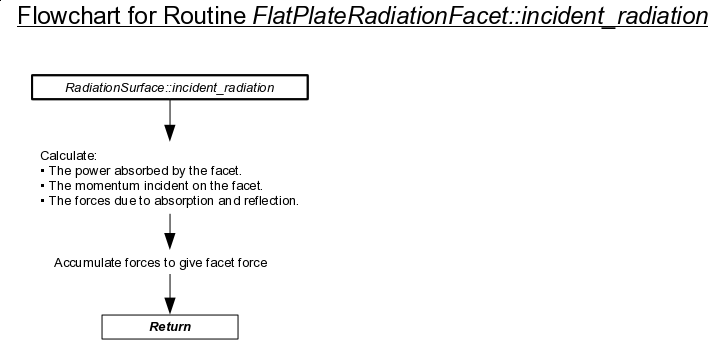
\includegraphics[width = 6 in]{figs/flowchart/flow_FP_incident_radiation.png}
  \label{fig:flow_FP_incident_radiation}
  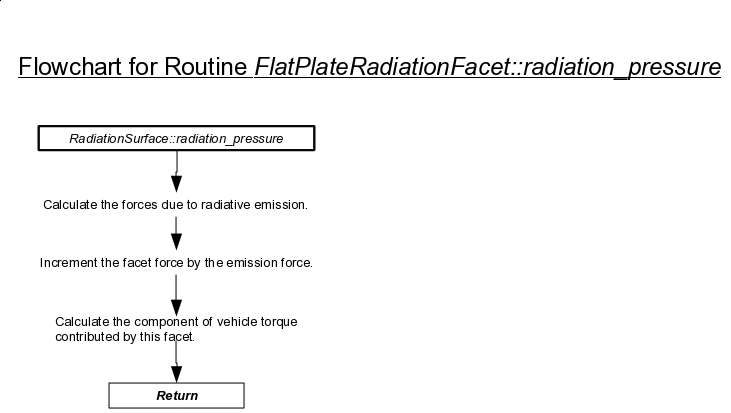
\includegraphics[width = 6 in]{figs/flowchart/flow_FP_radiation_pressure.png}
  \label{fig:flow_FP_radiation_pressure}
  \caption{Flowcharts for class FlatPlateRadiationFacet }
  
\end{figure}
Links: \newline
\textref{RadiationSurface::incident\_radiation}{fig:flow_incident_radiation}\newline
\textref{RadiationSurface::radiation\_pressure}{fig:flow_radiation_pressure}\newline
\clearpage

\begin{figure}[!ht]
  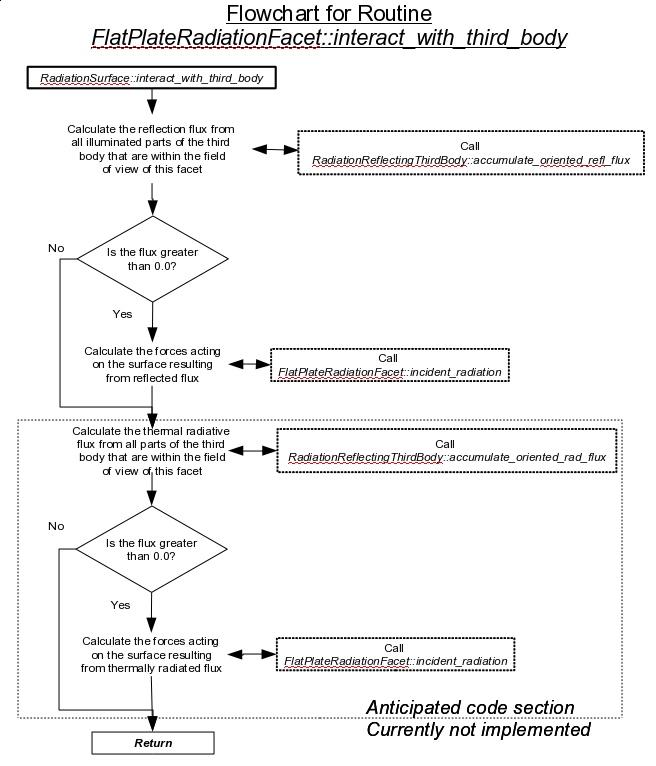
\includegraphics[width = 6 in]{figs/flowchart/flow_FP_interact_with_third_body.png}
  \label{fig:flow_FP_interact_with_third_body}
  \caption{Flowcharts for class FlatPlateRadiationFacet (continued)}
  
\end{figure}
Links: \newline
\textref{RadiationSurface::interact\_with\_third\_body}{fig:flow_interact_with_third_body}\newline
\textit{RadiationReflectingThirdBody::accumulate\_refl\_flux}(not implemented) \newline
\textref{FlatPlateRadiationFacet::incident\_radiation}{fig:flow_FP_incident_radiation}\newline
\textit{RadiationReflectingThirdBody::accumulate\_rad\_flux}(not implemented)
\clearpage

\begin{figure}[!ht]
  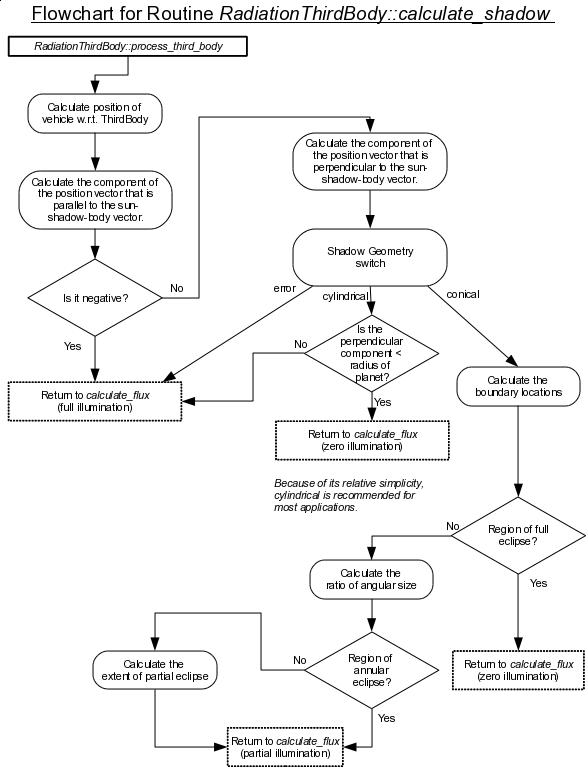
\includegraphics[width = 5.8 in]{figs/flowchart/flow_calculate_shadow.png}
  \caption{Flowchart for class RadiationThirdBody }
  \label{fig:flow_calculate_shadow}
\end{figure}
Links: \newline
\textref{RadiationSource::calculate\_flux}{fig:flow_calculate_flux}\newline
\clearpage

\begin{figure}[!ht]
  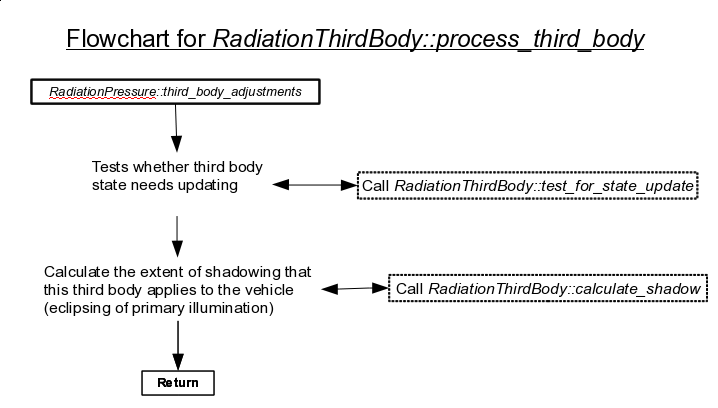
\includegraphics[width = 6 in]{figs/flowchart/flow_process_third_body.png}
  \label{fig:flow_process_third_body}
  
  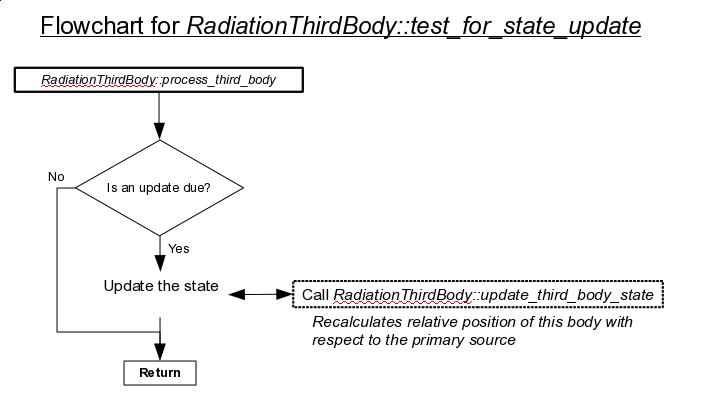
\includegraphics[width = 6 in]{figs/flowchart/flow_test_for_state_update.png}
  \label{fig:flow_test_for_state_update}
  \caption{Flowchart for class RadiationThirdBody (continued)}
  
\end{figure}
Links: \newline
\textref{RadiationPressure::third\_body\_adjustments}{fig:flow_third_body_adjustments}\newline
\textref{RadiationThirdBody::test\_for\_state\_update}{fig:flow_test_for_state_update}\newline
\textref{RadiationThirdBody::calculate\_shadow}{fig:flow_calculate_shadow}\newline
\textref{RadiationThirdBody::process\_third\_body}{fig:flow_process_third_body}
\clearpage

\begin{figure}[!ht]
  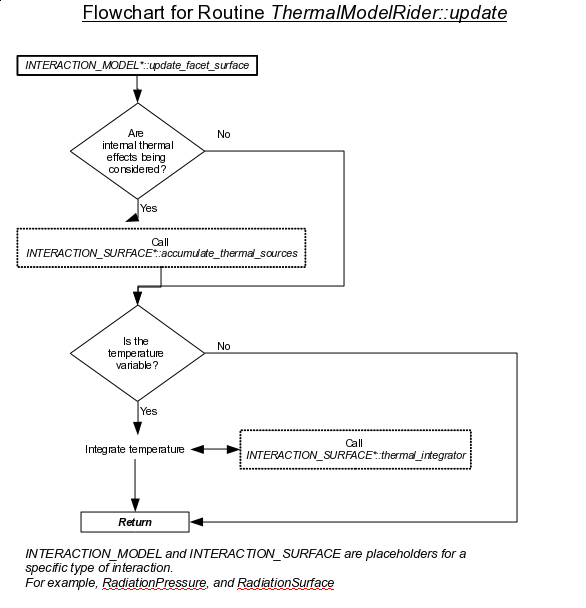
\includegraphics[width = 6 in]{figs/flowchart/flow_thermal_update.png}
  \caption{Flowchart for class ThermalModelRider }
  \label{fig:flow_thermal_update}
\end{figure}
Links: \newline
\textref{RadiationPressure::update\_facet\_surface}{fig:flow_update_facet_surface}\newline
\textref{RadiationSurface::accumulate\_thermal\_sources}{fig:flow_accumulate_thermal_sources}\newline
\textref{RadiationSurface::thermal\_integrator}{fig:flow_thermal_integrator}
\clearpage

\begin{figure}[!ht]
  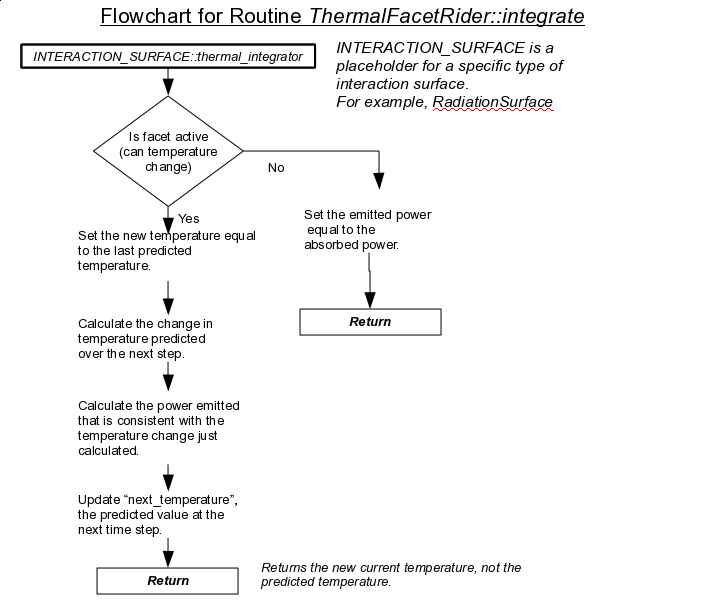
\includegraphics[width = 5.5 in]{figs/flowchart/flow_facet_thermal_integrate.png}
  \label{fig:flow_facet_thermal_integrate}
  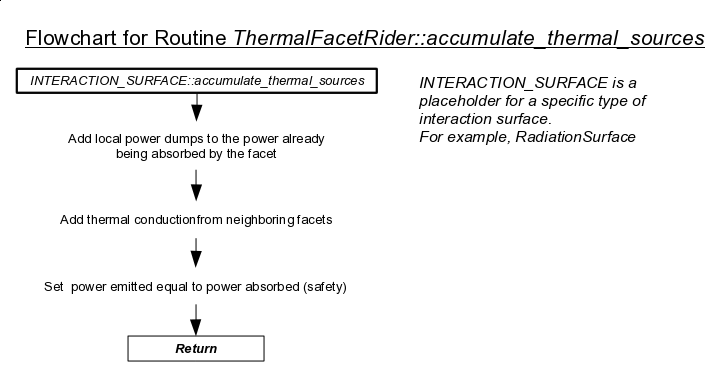
\includegraphics[width = 5.5 in]{figs/flowchart/flow_facet_accumulate_thermal_sources.png}
  \label{fig:flow_facet_accumulate_thermal_sources}
  \caption{Flowcharts for class ThermalFacetRider }
\end{figure}
Links: \newline
\textref{RadiationSurface::thermal\_integrator}{fig:flow_thermal_integrator}\newline
\textref{RadiationSurface::accumulate\_thermal\_sources}{fig:flow_accumulate_thermal_sources}\newline
\clearpage




\subsection{Functional Design} \label{sec:FunctionalDesign}
See the \href{file:refman.pdf}{Reference Manual} \cite{radbib:ReferenceManual}
 for a summary of member data and member methods for all classes.  This section
  describes the functional operation of the methods in each class.

Methods are ordered alphabetically within the class in
which they reside; classes are ordered alphabetically.
Methods that are inherited from a parent class
are described in that parent class.

Throughout this description, some words are used in both a generic sense, and as
particular instances of objects within the code, e.g. ``facet''.  Generally, an
attempt has been made to capitalize those instances that imply a specific case
of an object, and leave the generic term in lower case.  As a pedantic example:
a surface comprises a number of facets, and each Interaction Surface comprises a
number of Interaction Facets, each of which is associated with a Facet; each
 Facet contains the details of each
facet.

{\begin{enumerate}

\classitem{FlatPlateRadiationFacet}
 RadiationFacet

\begin{enumerate}

\funcitem{incident\_radiation}
Calculates the energy incident on the facet (\textit{areaxflux\_e}), and from
 that the rate at which energy is being absorbed.

If the model is being called only to manage the thermal aspect, it is complete.
Otherwise, it continues to calculate the momentum incident on the facet
(\textit{areaxflux)}, and from that the forces due to absorption, diffuse
reflection, and specular reflection.  The values calculated are added to
the preexisting values (which are initialized to zero at every time-step)
to allow this same method to be used for multiple sources.

\funcitem{initialize}
Assigns a pointer from the thermal facet rider to here, calls the thermal facet
rider initialization routine, and calculates the vector from the center of
rotation (center of mass, identified as \textit{center\_grav} in the model) to
the center of pressure of the facet.

\funcitem{define\_facet}
Copies the normal vector and the facet location into the appropriate variables.

\funcitem{interact\_with\_third\_body}\label{method:FPinteractwiththirdbody}
This method is used to add in the effects of reflective flux coming from
another body (referred to as a third-body).  It is called from the
\textit{RadiationSurface::interact\_with\_third\_body} method, which in turn is
called from the \textit{RadiationPressure::update\_facet\_surface} method; from
there, it receives a pointer to a RadiationThirdBody.  Since the call is
restricted to when the RadiationThirdBody is flagged as
\textit{is\_interactive}, this pointer must actually be to a
RadiationReflectingThirdBody (a derivative class of RadiationThirdBody).  Note
also that this method is called \textit{for each plate} for each instance of an
\textit{interactive} RadiationThirdBody.

The RadiationReflectingThirdBody is not released as a supported component of
JEOD, but the developed (currently undergoing testing) concept is for the
third-body to keep track of what elements of its surface are both illuminated
and visible to the vehicle.  This method makes a call to the third-body
\textit{accumulate\_oriented\_refl\_flux} method to accumulate the incident
flux from that part of its illuminated visible (i.e. visible to the vehicle)
surface that would be visible to this specific facet.  The determination of
which parts of the third-body surface are visible to this facet (as opposed to
the vehicle in general) is made by considering the orientation of the facet,
identified by its \textit{normal}.  This new value for flux is then passed into
the \textit{incident\_radiation} method, where its effect is added to that from
the primary source flux.

A secondary aspect of this method is to accumulate the thermal radiative flux
from the third-body.  This method is still undergoing development.
Conceptually, it is more simple than the reflective flux, since the entire body
is radiating, so there is no ``illuminated'' field to evaluate, just the field
of view from the facet.  However, the wavelength-profile of that radiation is
substantially different than that for the visible radiation previously
considered for the primary and reflected fluxes. Consequently, most materials
are likely to have a different albedo for this infrared radiation, and the
albedo plays a very large role in the \textit{incident\_radiation} method.
However, the primary purpose of this calculation is to model the thermal
contribution of this radiation because the flux is typically very weak, so
typically has only a negligible dynamic effect. Indeed, in order for the
dynamic effect to be adequate to cause a significant shift in the trajectory,
the vehicle would have to be sufficiently close to the body as to make
aerodynamic forces so dominant that the dynamic effect from radiative flux
would be lost in the noise of the aerodynamics.  Consequently, a temporary fix
to this problem is provided by adjusting the flux to accommodate the change in
albedo when calculating the absorbed power, and turning off the force
calculations (the force calculations use albedo in a way that is inconsistent
with the manipulation that permits its use for absorption calculations).

\funcitem{radiation\_pressure}
This method is called after all sources have been considered.  It uses the
recorded value of
emitted power to derive the force due to thermal
emission.   The four forces -- absorption; specular and diffuse reflection; and
emission -- are summed together to provide the total facet force, \textit{force}.
Torque is calculated
by considering the total force for the facet.

\funcitem{initialize\_runtime\_values}
This method simply zeros out the absorbed power, and the forces due to
absorption and reflection at the start of each time step.  This allows for the
incremental calculation of these elements.


\end{enumerate}


\classitem{FlatPlateRadiationFactory}
 InteractionFacetFactory (Surface Model)


\begin{enumerate}

\funcitem{create\_facet}
This method takes the defined Facet, and generates a Radiation Facet from it.
Each Facet has a set of parameters (\textit{FacetParams}) associated with it.
First, a check is made that the set of parameters is actually a set of
Radiation Parameters, and that the Facet is actually a Flat Plate Thermal Facet
(i.e., a flat plate with a Thermal Rider).  If either test fails, the code
cannot proceed.

Each Flat Plate Radiation Facet can see the base-class (Facet) data; that
pointer is set.  Then two initialization routines are called, one to initialize
the radiation aspects of the facet, and one to initialize the flat plate
aspects.

\funcitem{ is\_correct\_factory}
This method simply returns a true or false depending on whether the factory is
being passed an appropriate facet type.


\end{enumerate}


\classitem{RadiationDefaultSurface}
 Base-class


\begin{enumerate}

\funcitem{initialize}
Runs several tests to ensure that the initialization data is self-consistent
and valid, and calls the thermal facet rider initialization routine.

\funcitem{incident\_radiation}
Calculates the energy incident on the facet (\textit{areaxflux\_e}), and from
that the rate at which energy is being absorbed.

If the model is being called only to manage the thermal aspect, it is complete.
Otherwise, it continues to calculate the momentum incident on the facet
(\textit{areaxflux}), and from that the forces due to absorption, diffuse
reflection, and specular reflection.  The three forces are accumulated into one
value, and incremented to the value \textit{force} (this is initialized to zero
at each timestep; incrementing allows the same method to be used for multiple
sources).

\funcitem{interact\_with\_third\_body}
This method follows the same outline as that presented for the
\textref{FlatPlateRadiationFacet}{method:FPinteractwiththirdbody}, with the
exceptions that:

\begin{itemize}
 \item this method is called from the
 \textit{RadiationPressure::update\_default\_surface} method, not the
 \textit{RadiationPressure::update\_facet\_surface} method.
 \item The calls are to \textit{accumulate\_refl\_flux} and
 \textit{accumulate\_rad\_flux}; these are slightly different since the default
 surface has no orientation dependency.
\end{itemize}

Otherwise, the issues and restrictons are identical.
\end{enumerate}


\classitem{RadiationFacet}
 InteractionFacet (Surface Model)


\begin{enumerate}

\funcitem{initialize}
   Pure virtual function, must be defined in subclasses
\funcitem{radiation\_pressure}
   Pure virtual function, must be defined in subclasses
\funcitem{incident\_radiation}
    Pure virtual function, must be defined in subclasses
\funcitem{define\_facet\_core}
Extracts the data from the facet parameter set, and assigns it to the a
ppropriate variables in the facet data structure.  This includes data residing
in the Thermal Facet Rider.

\end{enumerate}


\classitem{RadiationMessages}
 Base-class

This is the message handler for the \RadiationPressureDesc.  It has no methods.

\classitem{RadiationParams}
FacetParams (Surface Model)

This class simply contains member data used to describe the radiative
properties of each facet in the Radiation Surface.  It has no methods.


\classitem{RadiationPressure}
 Base-class


{\begin{enumerate}

\funcitem{initialize}
There are two instances of the initialize function, differentiated by the
arguments they take.  One is used when the desired surface is the simple
default surface, and the other when the desired surface is a full Surface Model.

Both methods behave essentially the same:
\begin{enumerate}
 \item The dynamics manager pointer is set.
 \item To provide compatibility with older versions (where the
 RadiationThirdBody objects were recorded in the RadiationSource object), any
 ThirdBody objects stored in the RadiationSource object are copied over to the
 RadiationPressure object, along with the shadow geometry (which used to be
 common to all RadiationThirdBody objects).
 \item The environment is initialized with a call to initialize\_environment.
 \item The surface is initialized, with a call to the appropriate method.
\end{enumerate}


\funcitem{initialize\_environment}
First, the primary source is initialized, then assigned to all
RadiationThirdBody objects.  Each RadiationThirdBody object is then
initialized, which includes instructions to the Dynamics Manager to subscribe
to the appropriate reference frame to ensure that the frame is updated as
needed.

\funcitem{update}
This is the top-level method in the \RadiationPressureDesc.

The time-step is obtained from the simulation engine suing the interface method
\textit{get\_job\_cycle} and the Time Model's \textit{scale\_factor}.

Next, a call is made to calculate the incident flux from the primary source;
this is immediately followed up with a call to identify the modifications to
that flux that the RadiationThirdBody objects provide.

Finally, with the net flux available, a call is made to update the surface.

\funcitem{third\_body\_adjustments}
This method calls each RadiationThirdBody object's
\textit{process\_third\_body} method, which returns the fraction of the primary
source that the RadiationThirdBody is eclipsing.  These values are multiplied
together, using the assumption that no eclipses overlap.  The final value is
used to modify the incident flux, previously calculated.


\funcitem{update\_default\_surface}
This method is a simplified version of the method
\textref{update\_facet\_surface}{method:updatefacetsurface}.  It processes the
same calculations to identify the incident flux.  Then because there is only
one facet, the only thermal update to carry out is the potential for dumping
thermal energy from some internal power source.  The temperature is then
integrated if necessary.  Because the surface is isothermal, there is no net
thermal emission force, and because the surface is spherical, there is no
torque.


\funcitem{update\_facet\_surface}\label{method:updatefacetsurface}
This method processes the following steps:

{\begin{enumerate}
\item Set to zero the absorbed power, and the forces due to absorption, and
specular and diffuse reflection on each facet with a call to the
\textit{RadiationSurface::initialize\_runtime\_values} method.  The power and
force components are incremented during the processing of the
\RadiationPressureDesc, so must start at zero.

\item A call is made to \textit{RadiationSurface::incident\_radiation} to
process the forces resulting from absorption and reflection of light direct
from the primary source (Sun).  The flux from the primary source has already
been calculated.

\item For each registered RadiationThirdBody that is also interactive (i.e. is
a RadiationReflectingThirdBody) and is active (i.e. typically this means that
it is in the vicinity of the vehicle), the interactions with the flux reflected
and/or radiated from that body are calculated (see
\textref{interact\_with\_third\_body}{method:interactwiththirdbody}).

\item The thermal rider is updated.  The primary purpose of this call is to
integrate the temperature; this may seem unnecessary if the user does not wish
to maintain an evolutionary profile of the temperature.  However, this method
also contains the methods to add thermal energy from within the vehicle.  Then,
if the temperature is dynamic, it is integrated and the emitted power obtained.
 If the temperature is to be held fixed, the method
 \textit{equalize\_absorption\_emission} is called to set the emitted power
 equal to the absorbed power, but after internal energy sources have been added
 to the surface.

\item With the emitted power now available, the force due to thermal emission
can be calculated if forces are desired (see
\textref{radiation\_pressure}{method:surfaceradiationpressure}.  With the
emission force calculated, all forces are known; the surface accumulates all
forces and corresponding torques from all facets into an overall surface force.
 Those data are copied into the model force and torque.

\end{enumerate}}


\funcitem{add\_third\_body}
The RadiationPressure class keeps a record of all RadiationThirdBody objects
that could influence the raw flux between the primary source (Sun) and target
(the vehicle with which the particular instance of the RadiationPressure model
is associated).  The primary role of this method is to verify that
RadiationThirdBody objects have been initialized correctly, and if so, to add
them to the list (vector) of RadiationThirdBody objects.  It includes
verification that the object exists, is named with a unique name (within this
model), and has not previously been added to any other RadiationPressure model
(because the RadiationThirdBody can see the model's RadiationSource data, and
RadiationSource contains data about the source-vehicle position, each
RadiationThirdBody object can be associated with only one vehicle, and
consequently, only one RadiationPressure model).

The actual registration involves a test of casting to a
RadiationReflectingThirdBody.  This class is not implemented in this release of
JEOD, but provides the foundation for future addition of an albedo model.

Although this method is typically called during simulation setup
(pre-initialization), it can be called at any time in the simulation.  Hence,
if the model has already been initialized, it is necessary to initialize this
third-body (otherwise, the initialization will be performed as an integral
aspect of the model initialization).

Finally, if any third-body objects are flagged as being active, the model flag
must be set accordingly.

\funcitem{set\_third\_body\_active}
RadiationThirdBody objects may be listed with the RadiationPressure model, but
inactivated.  This means that they will not be considered when calculating the
effect of the third-bodies.  This method changes the state of a
RadiationThirdBody from inactive to active; the RadiationThirdBody is
identified by name.


\funcitem{set\_third\_body\_inactive}
See \textit{set\_third\_body\_active} immediately above.  This method works in
reverse.

\funcitem{find\_third\_body}
This simple method identifies the location in the vector of third-body pointers
of a particular instance, identified by name.

\funcitem{set\_calculate\_forces}
This method is used to set the \textit{calculate\_forces} flag.  Note that the model force and torque will not be calcualted if this is set to false.  Consequently, it is essential that these values be set to zero with the flag being turned off, lest the last value be retained and included for all time.
\end{enumerate}}


\classitem{RadiationSource}
 Base-class


{\begin{enumerate}

\funcitem{initialize}
Identifies the source by name (most often ``Sun''), and ensures that the
Dynamics Manager maintains its position information.


\funcitem{calculate\_flux}\label{ref:calculateflux}
The incident flux is governed by an inverse-square law applied to the
illuminating source over the distance between source and vehicle, with
additional factoring to account for intervening bodies that could cause
shadowing or eclipses.

The distance from source to vehicle is determined, and the raw flux
determined as a vector in the inertial and the vehicle structural reference
frames, and as a magnitude.

\end{enumerate}}


\classitem{RadiationSurface}
 Interaction Surface (Surface Model)

A Radiation Surface is a surface derived from the Surface Model.  A Radiation
Default Surface is another class entirely, and is used for simple, crude
application of radiation pressure theory.  The methods presented in this class
are only applied to a Radiation Surface, and never to a Radiation Default
Surface.
{\begin{enumerate}

\funcitem{initialize}
Contains a sequence of calls and checks to initialize each of the facets that
comprise the surface, and verify the suitability of the data in each facet.

\funcitem{allocate\_array}
Allocates the memory for the Radiation Facets.

\funcitem{allocate\_interaction\_facet}
Calls the appropriate factory to generate Radiation Facets from the base
Facets, and checks that the generation was consistent.

\funcitem{incident\_radiation}
Calls the Radiation Facet method \textit{incident\_radiation} on each Radiation
Facet in turn.

\funcitem{interact\_with\_third\_body}\label{method:interactwiththirdbody}
Calls the Radiation Facet method \textit{interact\_with\_third\_body}  on each
Radiation Facet in turn.  See, for example,
\textref{FlatPlateRadiationFacet::interact\_with\_third\_body}{method:FPinteractwiththirdbody}.

\funcitem{accumulate\_thermal\_sources}
Calls the Thermal Facet Rider method \textit{accumulate\_thermal\_sources} on
each Radiation Facet in turn.

\funcitem{thermal\_integrator}
Calls the Thermal Facet Rider method \textit{integrate} on each Radiation Facet
in turn.

\funcitem{equalize\_absorption\_emission}
Sets the Thermal Facet Rider value \textit{power\_emit} equal to the Thermal
Facet Rider value \textit{power\_absorb} for each Radiation Facet in turn.

\funcitem{radiation\_pressure}\label{method:surfaceradiationpressure}
Calls the Radiation Facet method \textit{radiation\_pressure} on each Radiation
Facet in turn.  Sums the forces and torques from each facet into a force and
torque for the surface as a whole.  Note that this method is only called from
the main model function call if the flag \textit{calculate\_forces} is set.

\funcitem{initialize\_runtime\_values}
Calls the Radiation Facet method \textit{initialize\_runtime\_values} on each
Radiation Facet in turn.

\end{enumerate}}


\classitem{RadiationSurfaceFactory}
 InteractionSurfaceFactory (Surface Model)


{\begin{enumerate}

\funcitem{add\_facet\_params}
Checks that the parameter list is a Radiation Parameter list, and calls the
generic Interaction Surface Factory method \textit{add\_facet\_params}.
\end{enumerate}}


\classitem{RadiationThirdBody}
Base Class

A Third Body is an object that is neither the vehicle nor the primary
illumination source (usually Sun).  It can shadow the vehicle, and potentially
reflect light onto the vehicle from the primary illumination source.

{\begin{enumerate}

\funcitem{initialize}
Identifies the Dynamics Manager's memory allocation for the physical object
that this third-body is representing, and makes sure that the Dynamics Manager
will maintain up-to-date information about its state.

Calculates some radii comparisons that are used in the conical shadowing
calculation.


\funcitem{process\_third\_body}
This is the primary executable for handling the ThirdBody shadowing effects.  In many applications, it is not necessary to update the position and orientation of the third-body as rapidly as that of the vehicle.  Particularly in the case where a third-body presents a complex albedo map for reflected radiation, that update can be unnecessarily time-consuming.  The first task is to query whether the state of the third body requires an update, with a call to \textit{test\_for\_state\_update} (note, this method will perform the update if it is necessary).  Next, the shadow that the body casts is evaluated based on its most recent state.

\funcitem{calculate\_shadow}
See Figure~\ref{fig:flow_calculate_shadow} for a flow chart of how this method
is processed, and sections \textref{Reduction of Flux by Intervening
Body}{ref:shadowcalculator} and \textref{Conical Eclipse
Calculator}{sec:conicaleclipsecalculator} for a complete mathematical treatment
of this algorithm.

In summary of the method, the following steps are taken:
{\begin{enumerate}
\item The position vector of the Third Body with respect to the primary source
is calculated (\textit{source\_to\_third}), and decomposed into magnitude and
unit vector.
\item The position vector of the vehicle with respect to the Third Body is
calculated (\textit{third\_to\_cg}).
\item The component of \textit{third\_to\_cg} that is parallel to
\textit{source\_to\_third} is calculated (\textit{r\_par}).  If $r\_par < 0$,
the vehicle is ``in front'' of the Third Body and cannot be shadowed by it.
\item The component of \textit{third\_to\_cg} that is perpendicular to
\textit{source\_to\_third} is calculated (\textit{r\_perp}).
\item The user has two options for the geometry of the shadow:

{\begin{itemize}
\item A \textit{cylindrical} shadow blocks out the cross section of the Third
Body parallel to \textit{source\_to\_third}, extending to infinity.
\item A \textit{conical} shadow treats the lines extending from the limbs of
the illuminating body to the limbs of the Third Body to determine whether all,
part, or none, of the illuminating disk is obscured.  This method is described
in section \textref{Conical Eclipse Calculator}{sec:conicaleclipsecalculator}.
\end{itemize}}
\item Full or zero obscuration are easy to handle, but the situation in which
part of the disk is obscured is more challenging.  To avoid multiple inverse
trigonometric functions, a description has been developed utilizing a 3rd order
polynomial, with 2nd or 3rd order polynomial coefficients.
\end{enumerate}}

\funcitem{test\_for\_state\_update}
If sufficient time has elapsed since the last time the state was updated (as
determined by a user-defined value, \textit{update\_interval}), update the
state, and record the time.

\funcitem{update\_third\_body\_state}
Generates the position of the third body with respect to the primary source.
For a generic RadiationThirdBody, orientation is not necessary.

\funcitem{convert\_shadow\_from\_int}
This method is used to ensure compatibility between the old paradigms in which
the RadiationThirdBody objects are contained within the RadiationSource, and
the new paradigm in which they are stand-alone objects registered with the
RadiationPressure model.  The shadow geometry enumeration is located
differently for these two paradigms; this method moves the older implementation
to the new enumeration.

\funcitem{accumulate\_refl\_flux}
For a generic RadiationThirdBody object, there is no reflection flux from its
surface.  This method is provided to allow for extension of an albedo model to
a RadiationDefaultSurface, but for this class, it returns 0.0.

\funcitem{accumulate\_rad\_flux}
For a generic RadiationThirdBody object, there is no radiative flux from its
surface.  This method is provided to allow for extension of a thermal radiation
model to a RadiationDefaultSurface, but for this class, it returns 0.0.

\funcitem{accumulate\_oriented\_refl\_flux}
For a generic RadiationThirdBody object, there is no reflection flux from its
surface.  This method is provided to allow for extension of an albedo model to
a RadiationSurface, but for this class, it returns 0.0.

\funcitem{accumulate\_oriented\_refl\_flux}
For a generic RadiationThirdBody object, there is no radiative flux from its
surface.  This method is provided to allow for extension of a thermal
radiation model to a RadiationSurface, but for this class, it returns 0.0.

\funcitem{is\_interactive}
This is used to distinguish between those third body objects that can generate
flux vectors (through radiative emission or reflection) from thise that cannot.
 This generic form of a RadiationThirdBody cannot.  Consequently, this method
 returns \textit{false}.

\funcitem{get\_added\_to\_model}
The \textit{added\_to\_model} flag gets set when an instance of a
RadiationThirdBody gets added to a RadiationPressure model.  It is essential
that a RadiationThirdBody object can only be in one RadiationPressure model.
It is possible to have multiple RadiationThirdBody objects that represent the
same object (e.g. for a 2-vehicle simulation around Earth, there may be two
RadiationThirdBody objects that represent Earth, once for each vehicle's
RadiationPressure model), but the same object must not be used twice.  The
\textit{added\_to\_model} protects against that.

\funcitem{set\_added\_to\_model}
See \textit{get\_added\_to\_model} immediately above.

\end{enumerate}}

\classitem{RadiationReflectingThirdBody}
 RadiationThirdBody

This derived class is left as a stub to allow for a third-body object to
contain an albedo model and provide a reflective and radiative flux to the
vehicle.  It is not currently implemented.

\end{enumerate}}

%\section{Version Inventory}
%%%%%%%%%%%%%%%%%%%%%%%%%%%%%%%%%%%%%%%%%%%%%%%%%%%%%%%%%%%%%%%%%%%%%%%%%%%%%%%%%
%
% Purpose:  Inventory of files for the RadiationPressure model
%
%
%%%%%%%%%%%%%%%%%%%%%%%%%%%%%%%%%%%%%%%%%%%%%%%%%%%%%%%%%%%%%%%%%%%%%%%%%%%%%%%%

\section{Inventory}
All \RadiationPressureDesc\ files are located in the directory \newline
{\tt \$\{JEOD\_HOME\}/models/interactions/radiation\_pressure}.
Relative to this directory,
\begin{itemize}
\vspace{-0.2\baselineskip}
\item Header and source files are located
in the model {\tt include} and {\tt src} subdirectories.
Table~\ref{tab:source_files} lists the
configuration-managed files in these directories.
\vspace{-0.1\baselineskip}
\item Data files are located in the model {\tt data} subdirectory.
See table~\ref{tab:data_files}
for a listing of the
configuration-managed files in this directory.
\vspace{-0.1\baselineskip}
\item Documentation files are located in the model {\tt docs} subdirectory.
See table~\ref{tab:documentation_files}
for a listing of the
configuration-managed files in this directory.
\vspace{-0.1\baselineskip}
\item Verification files are located in the model {\tt verif} subdirectory.
See table~\ref{tab:verification_files}
for a listing of the
configuration-managed files in this directory.
\end{itemize}

\input{inventory}


\chapter{User Guide}\hyperdef{part}{user}{}\label{ch:user}
%----------------------------------
The Analysis section of the User Guide is intended primarily for
users of preexisting simulations.
It contains:
\begin{itemize}
\item a description of how to modify \RadiationPressureDesc\ variables after
the simulation
has compiled, including an in-depth discussion of the input file,
\item an overview of how to interpret (but not edit) the S\_define
file,
\item a sample of some of the typical variables that may be logged.
\end{itemize}

The Integration section is intended for simulation
developers.
It describes the necessary configuration of the \RadiationPressureDesc\
within an
S\_define file, and the creation of standard run directories.  The
latter
component assumes a thorough understanding of the preceding Analysis
section.
Where applicable, the user may be directed to selected portions of
Product Specification (Chapter \ref{ch:spec}).

The Extension section is intended primarily for
developers
needing to extend the capability of the \RadiationPressureDesc.  Such users
should have a
thorough understanding of how the model is used in the preceding
Integration section, and of the model
specification (described in Chapter \ref{ch:spec}).


\section{Analysis}
%%%%%%%%%%%%%%%%%%%%%%%%%%%%%%%%%%%%%%%%%%%%%%%%%%%%%%%%%%%%%%%%%%%%%%%%%%%%%%%%%
%
% Purpose:  Analysis part of User's Guide for the RadiationPressure model
%
%
%%%%%%%%%%%%%%%%%%%%%%%%%%%%%%%%%%%%%%%%%%%%%%%%%%%%%%%%%%%%%%%%%%%%%%%%%%%%%%%%

% \section{Analysis}

\subsection{Identifying the Radiation Pressure Model}
If the radiation pressure model is included in your simulation, there must be an
instance declared of the class \textit{RadiationPressure}.  There must also be a
Radiation Surface through which the radiation field can interact with the
vehicle.  Searching the S\_define for ``RadiationPressure'' is a good strategy
for determining the presence of a Radiation Pressure model in the simulation.
Once identified, it is also necessary to identify which type of surface is being
used; there are two fundamentally different types of surface, the general
surface (the S\_define will contain an instance of a RadiationSurface) and the
model-specific, default surface (the S\_define will contain an instance of a RadiationDefaultSurface).

The default surface is defined by relatively few characteristics, so is more easily created, managed, and manipulated.  However, it is constrained to represent the effect of a spherical shell around the vehicle, so has limited applicability.  Because the default surface is so easily defined, the definition often resides in an input file.

The general surface uses the Surface Model to define the surface (see the Surface Model~\cite{dynenv:SURFACEMODEL} documentation for details on how this functions).  The basic premise of the surface model is that the actual vehicular surface can be represented as a combination of geometric surfaces, or facets (typically, these are flat plates).  The number of facets used to describe the surface depends on the complexity of the surface and the desired fidelity of the approximation.  Because the general surface can be significantly more complex, it is typically defined in a data file that is included into the input file.

\subsection{Editing the Radiation Pressure Model}
The model parameters and the individual parameters for the surface as defined can easily be edited.  It is also possible to replace one surface with another mid-simulation (for example, to increase the desired fidelity during particularly sensitive phases of the mission), although this requires knowledge of how to implement a surface, and is beyond the scope of the Analyst.  Details can be found in the Integration section of the User's Guide.

The description of the control is divided into model-wide control, surface element control, and illumination control.

\subsubsection{Model control}

The most important flag is the \textit{active} flag; this turns the radiation pressure model on or off.  This value defaults to true.

The following settings apply to the model as a whole:
\begin{itemize}
\item{\textit{calculate\_forces}, default = true}.  \newline
The \RadiationPressureDesc\ can be used to model surface temperature variations and forces resulting from the interaction of the vehicle surface with the radiation environment.  Turning this off restricts the scope to temperature only.
\end{itemize}

\subsubsection{RadiationThirdBody Control}
The frequency with which the RadiationThirdBody state is updated can be
manipulated.  This is more important for RadiationReflectingThirdBody items
than for generic RadiationThirdBody.  The value \textit{update\_interval}
specifies the minimum time interval between updates.  The state will be updated
at the call following passage of this time.  If this value is set to 0.0
(default), the state will be updated continuously.


\subsubsection{Default Surface Control}

The following values affect the behavior if the default surface:
\begin{itemize}
\item{Cross-sectional Area (\textit{cx\_area}, default = 0.0)}.
\item{Surface Area (\textit{surface\_area}, default = 0.0)}. \newline
The area of the surface can be defined in one of two ways -- either as a cross-sectional, or a surface area.  Since the default surface models a sphere, these differ by a factor of 4.  The user should not attempt to define both.

\item {Albedo (\textit{albedo}, default = -1.0)}. \newline
This is the fraction of light incident on the surface that is immediately reflected back away.  This value runs from 0.0 (matte black) to 1.0 (mirrored).

Either the radiation coefficient, or the combination of albedo and diffuse
parameter, must be specified for a default surface.  The negative default
settings on these values ensure that one \textit{and only one} valid entry is
made.

\item {Diffuse parameter (\textit{diffuse}, default = -1.0)}.\newline
This is the fraction of reflected light that is reflected diffusely; reflection can often be classified into specular or diffuse reflection, specular reflection is the type of reflection from a mirror, whereas diffuse reflection is the type of reflection off a matte surface.  A rough matte surface would have a diffuse parameter close to 1, while a highly polished surface would typically have a diffuse parameter closer to 0.

Either the radiation coefficient, or the combination of albedo and diffuse
parameter, must be specified for a default surface.  The negative default
settings on these values ensure that one \textit{and only one} valid entry is
made.

\item{Emissivity (\textit{thermal.emissivity}, default = 0.0)}. \newline
The emissivity measures how close to Planck-like Black Body radiation the thermal emission actually is.  This value is typically highly dependent on albedo, with the sum of the two terms approximately equal to 1.0.

\item {Heat Capacity (\textit{thermal.heat\_capacity}, default = 0.0)}.\newline
The heat capacity must be defined if the surface is thermally dynamic.  It is quite unreasonable to set some arbitrary number as a default setting, so 0.0 was assigned.  However, that means that the temperature of the surface can change without bound for an infinitesimal imbalance in the energy received and emitted (the vehicle requires 0.0 energy to change its temperature by each degree).  If this number is not at all known, the only safe option is to make the surface thermally static by turning off the active flag.

\item {Internal Sources (\textit{thermal.thermal\_power\_dump}), default =
0.0)}.\newline
If the vehicle has some source of internal thermal energy generation (e.g. some sort of reactor), this value would be set equal to the power input to the vehicle surface from that source.

\item {Radiation Coefficient (\textit{rad\_coeff}, default = -1.0)}.\newline
The radiation coefficient ($C_R$) provides an alternative method for specifying the
reflection parameters, using only one value instead of albedo ($\alpha$) and
diffuse ($\delta$).
Numerically,
\begin{equation*}
C_R = 1 + \frac{4}{9} \alpha \delta \in [1.000 , 1.444]
\end{equation*}
Either the radiation coefficient, or the combination of albedo and diffuse
parameter, must be specified for a default surface.  The negative default
settings on these values ensures that one \textit{and only one} valid entry is
made.

\item {Temperature (\textit{temperature}, default = 0.0)}.\newline
The extent to which radiation is absorbed and emitted has an effect on temperature, and vice versa.  Since the radiation model includes pressure from thermal radiative emission, it is important that the temperature is known to some level of accuracy.

\item {Thermally Dynamic (\textit{thermal.active}, default = true)}.\newline
Integration of the temperature is time-consuming and cumbersome.  If the vehicle is in a situation in which the surface temperature does not change appreciably, this value can be turned off to circumvent the integration.  In that case, the temperature of the vehicle will be constant in time.

\end{itemize}


\subsubsection{General Surface Control}
Each facet in the surface is assigned a set of physical and material properties.  The physical properties typically vary from facet to facet, but many facets may share the same material properties if they are fabricated of the same material.

\paragraph{Physical Properties} \ \newline
The following values are assigned to each facet in the surface.
\begin{itemize}
\item {Position (\textit{position}, 3-vector)}. \newline
The relative positions of the facets are necessary to generate torques.  If the surface is a fixed and immovable monolith, these values are typically expressed in the structural reference frame.
\item{Orientation (\textit{normal}, 3-vector, unit vector)}.  \newline
As the vehicle position and attitude changes, facets will tend to rotate in and out of sunlight.  The orientation allows the correct angle to the flux vector to be calculated.  This should be expressed in the same reference frame as the position.
\item{Area (\textit{surface\_area})}.
\item{Temperature (\textit{temperature})}.  \newline See Default Surface for explanation.
\item{Thermally Dynamic (\textit{thermal.active})}.  \newline
See Default Surface for explanation.
\item{Internal Sources (\textit{thermal.thermal\_power\_dump}}.  \newline See Default Surface for explanation.
\end{itemize}

\paragraph{Material Properties} \ \newline
Each facet contains an element, \textit{param\_name}, that identifies the material from which it is made.  Each set of parameters contains the following information:
\begin{itemize}
\item {Name (\textit{name})}. \newline
This matches the value of \textit{param\_name} in the facet.
\item{Albedo (\textit{albedo})}. \newline
See Default Surface for explanation.
\item{Diffuse Parameter(\textit{diffuse})}. \newline
See Default Surface for explanation.
\item{Emissivity (\textit{thermal.emissivity})}.  \newline
See Default Surface for explanation.
\item{Heat Capacity (\textit{thermal.heat\_capacity\_per\_area})}.  \newline
See Default Surface for explanation of the importance of heat capacity.  Because this is a material property, and heat capacity depends on the size of the facet, this value is defined as heat capacity per unit area, and internally converted into the heat capacity.
\end{itemize}


\subsubsection{Illumination Control}

The radiation source is assumed to be that of the sun.  This can be changed, by changing the values \textit{source.name, source.luminosity, source.radius}; however, it is recommended that these be left at the solar default settings.

The following controls are more typically changed:
\begin{itemize}
\item{\textit{third\_bodies[ii]$->$shadow\_geometry}, default = RadiationSource::Conical}.
\newline
This can take a value either Cylindrical (or Cyl) or Conical (or Con), and allows the user to switch between the true conical shadowing of an intervening body, and the simpler cylindrical shadowing.  It is not necessary to treat all third-body objects alike.
\item{\textit{third\_bodies[ii]$->$active}, default = true}. \newline
If the user wishes to include the effects of an intervening body, the method \textit{set\_third\_body\_active} must be run (and \textit{set\_third\_body\_inactive} will inactivate it again).  These methods will control the general flag, \textit{third\_bodies\_active}.
The flag is user-controllable, and can be manually set, but should not be (unless the user really knows what he or she is doing).
\item{\textit{third\_bodies\_active}, default = false}. \newline
If the \textit{third\_bodies\_active} flag is set, then any registered and active third-bodies (e.g., Earth) will be processed for affect on the raw flux.
IMPORTANT NOTE -- there is no reason to change this flag manually.  If the third bodies are activated/inactivated using the provided methods, then this flag is automatically controlled (on when any number of third bodies is active, off when all third-bodies are inactive).
\end{itemize}


\subsection{Output Data}
The primary output data of the \RadiationPressureDesc\ are the values:
\begin{itemize}
\item{\textit{force}}
\item{\textit{torque}}
\end{itemize}

Also available are the forces due to each interaction process across the surface.

\begin{itemize}
\item{\textit{rad\_surface.F\_absorption}}
\item{\textit{rad\_surface.F\_specular}}
\item{\textit{rad\_surface.F\_diffuse}}
\item{\textit{rad\_surface.F\_emission}}
\item{\textit{rad\_surface.force}}
\item{\textit{rad\_surface.torque}}
\end{itemize}

IMPORTANT NOTE -- the model \textit{force} and \textit{torque} are more reliable than the surface versions (\textit{rad\_surface.force} and \textit{rad\_surface.torque}).  In most applications, they are identical.  The distinction comes only when an active model is turned off.  The model values will be reset to zero, but the surface values will retain their old value.  The model values should be used preferentially over the surface values.

The same data is calculated and can be extracted for each individual facet,
along with the temperature of the facet.  These individual facet data cannot be
directly recorded in a regular Trick simulation, but are indirectly available.
An example of how to record these data is shown in
\textit{verif/SIM\_2\_SHADOW\_CALC/Log\_data\_radiation\_rec.d}, using the
additional object \textit{radiation.data\_rec}, an instance of
RadiationDataRecorder.  This functionality requires an additional function call
to \textit{radiation.data\_rec.record\_data} from the S\_define, and can be found in SIM\_2\_SHADOW\_CALC, SIM\_3\_ORBIT, and SIM\_4\_DEFAULT.
The additional functionality and class are defined in the verification section
of the model, and are made available to the user, but are not intended to be an
integral part of the \RadiationPressureDesc.


%\section{Integration}
%%%%%%%%%%%%%%%%%%%%%%%%%%%%%%%%%%%%%%%%%%%%%%%%%%%%%%%%%%%%%%%%%%%%%%%%%%%%%%%%%
%
% Purpose:  Integration part of User's Guide for the RadiationPressure model
%
%
%%%%%%%%%%%%%%%%%%%%%%%%%%%%%%%%%%%%%%%%%%%%%%%%%%%%%%%%%%%%%%%%%%%%%%%%%%%%%%%%

 \section{Integration}

Including the \RadiationPressureDesc\ is a straightforward process, the most
complicated part of which is in generating the Radiation Surface.  For working
examples, the integrator is strongly encouraged to view the simulations in the
\RadiationPressureDesc\ verification.

Note that a \RadiationPressureDesc\ is vehicle-specific.  In multi-vehicle
simulations, it is necessary to have one \RadiationPressureDesc\ per vehicle
(or, at least, per vehicle for which radiation pressure is important).

\subsection{Generating the S\_define}

The following steps provide a consistent method for integrating Radiation
Pressure into the simulation:
\begin{enumerate}
  \item{} Declare a simulation object, called \textit{radiation} or similar, in
  the
         S\_define or equivalent file.
  \item{} Within the simulation object, declare instances of the following
  classes:
  \begin{enumerate}
    \item{RadiationPressure}. \newline
      For Trick07 simulations, the preferred implementation
      of RadiationThirdBody
      objects (a third-body is one that is
      neither the vehicle nor the source of illumination, e.g., the sun,
      but can still contribute to the effect of radiation pressure)
      is as an array located in the RadiationSource object.  In this case,
      this array must be populated with information
      on the primary source of illumination, and on any third-bodies.
      In the \JEODid\ release, there are two data files (at
      \textit{models/interactions/radiation\_pressure/data} that can be used as
      templates; one (\textit{sun.d}) recognizes Sun only,
      the other (\textit{sun\_earth\_moon.d}) recognizes Sun as the primary
      source of illumination, and Earth and Moon as third-bodies.

      For Trick10 simulations, the preferred method of implementing
      RadiationThirdBody objects is to instantiate them as stand-alone objects,
      and register them with the RadiationPressure model.  This method is
      generally preferred, and the registration is implemented
      behind-the-scenes even in Trick07 simulations.  In this case, there is no
      default data to add to the radiation pressure model, but instead the data
      is entered at the input level.  See, for example,
      \textit{verif/SIM\_1\_BASIC\_T10/Modified\_data/third\_bodies.py} which
      sets up Earth and Moon as third-bodies much the same as
      \textit{sun\_earth\_moon.d} did in the older paradigm.

    \item{} Either one of:
      \begin{itemize}
        \item{RadiationSurface} or
        \item{RadiationDefaultSurface}
      \end{itemize}
      A simulation object should not contain both of these,
      nor should it contain multiple examples of either one,
      unless the intent is to use those sequentially.
      One instance of RadiationPressure can use only one surface at a time.
      Users wishing to compare the effect of different surfaces should use
      multiple simulation objects, each with its own instance of
      RadiationPressure.
    \item{} If the RadiationSurface option is used,
      also instantiate the following classes / class pointers:
      \begin{enumerate}
        \item{RadiationSurfaceFactory}
        \item{SurfaceModel} (located at \textit{utils/surface\_model})
        \item{Facet **} \newline
          An array of pointers to the facets
          (\textit{Facets} are at \textit{utils/surface\_model}).
        \item{\textit{$<$facet-type$>$} *} \newline
          An array of facets of
          type \textit{$<$facet-type$>$}, for example, \textit{FlatPlateThermal~*}
          These are probably also at \textit{utils/surface\_model}, unless the
          Surface Model has been extended to provide other facet-types
          that have been stored elsewhere.
        \item{} An unsigned integer (unassigned value, not necessary for Trick10)
        \item{RadiationParams *}
        \item{FacetParams *} .
      \end{enumerate}
        Note that none of these are initialized with data;
        the data are included from the input file as necessary.
    \item{RadiationDataRecorder \textit{(optional)}}. \newline
      Use this if it is also
      desirable to monitor the interaction at the facet level,
      rather than the model level.
      Note that this is only available if using a RadiationSurface and not used
      at all if implementing a RadiationDefaultSurface.
  \end{enumerate}
  \item{} Also within the simulation object, schedule the following jobs:
    \begin{itemize}
      \item{Pre-initialization}.  \newline
        If the Surface Model is being used,
        the surface must be created before initialization.  In Trick10, this can be done from the python input file.  In Trick07, this requires the advance declaration of the jobs that will be called from the input files.  This is a
        potentially confusing area for integration, because
        these jobs appear as environment class jobs, but are assigned a zero
        call rate to ensure that they never get called from the S\_define.
        Instead, they are called from the input file where the data are entered,
        but the methods must still be declared in the S\_define in order to be
        called from the input file.
        If the Default Surface is being used, or if the simulation engine can handle direct calls from the input-level files (e.g. Trick10, but not Trick07), then these calls should not be included.
        In the following example the variables being referred to map to the
        following list of previously defined items:
        \begin{itemize}
          \item \textit{radiation} is the simulation object
          \item \textit{facet\_ptr} is the instance of \textit{Facet **}
          \item \textit{integer} is the unsigned integer
          \item \textit{facet\_params} is the instance of \textit{FacetParams *}
          \item \textit{surface} is the instance of SurfaceModel
          \item \textit{rad\_surface} is the instance of the radiation surface, be that a
             RadiationSurface or a RadiationDefaultSurface
        \end{itemize}
\begin{verbatim}
(0.0, environment) utils/surface_model:
radiation.surface.add_facets(
        In Facet**      new_facets     = radiation.facet_ptr,
        In unsigned int num_new_facets = radiation.integer);

(0.0, environment) interactions/radiation_pressure:
radiation.surface_factory.add_facet_params(
       In FacetParams*  to_add         = radiation.facet_params);
\end{verbatim}

      \item {Initialization}
        \begin{enumerate}
          \item{} If the Surface Model is being used,
            the Radiation Surface must be created from the Surface.
\begin{verbatim}
(initialization) interactions/radiation_pressure:
radiation.surface_factory.create_surface(
    In SurfaceModel        * surface       =  &radiation.surface,
    Out InteractionSurface * inter_surface =  &radiation.rad_surface);
\end{verbatim}
          \item{} Whether the Surface Model or the Default Surface is being
            used, the \RadiationPressureDesc\ must then be initialized.
            The initialization call differs slightly for the two cases:
            \begin{itemize}
              \item{Surface Model}
\begin{verbatim}
(initialization) interactions/radiation_pressure:
radiation.rad_pressure.initialize(
       In  DynManager       & dyn_mgr        = mngr.dyn_manager,
       In  RadiationSurface * surf_ptr       = &radiation.rad_surface,
       In  double  center_grav[3] =
                      vehicle.dyn_body.composite_properties.position);
\end{verbatim}
              \item{Default Surface}
\begin{verbatim}
(initialization) interactions/radiation_pressure:
radiation.rad_pressure.initialize(
       In  DynManager              & dyn_mgr  = mngr.dyn_manager,
       In  RadiationDefaultSurface * surf_ptr = &radiation.rad_surface);
\end{verbatim}
            \end{itemize}
        \end{enumerate}


      \item {Scheduled jobs}
        \begin{enumerate}
          \item {Update values}
\begin{verbatim}
(DYNAMICS, scheduled)  interactions/radiation_pressure:
radiation_simple.rad_pressure.update(
       In  RefFrame & veh_struc_frame = vehicle.dyn_body.structure,
       In  double     center_grav[3]  =
                             vehicle.dyn_body.composite_properties.position,
       In  double     scale_factor    = time.manager.dyn_time.scale_factor);
\end{verbatim}

          \item{Record data (\textit{optional})}. \newline
            Used only with a Surface Model,
            and only if facet-specific data must be recorded.
\begin{verbatim}
(DYNAMICS, scheduled)  interactions/radiation_pressure/verif:
radiation.data_rec.record_data (
     In  RadiationSurface * surface_ptr = &radiation.rad_surface);
\end{verbatim}
        \end{enumerate}
    \end{itemize}
\end{enumerate}


\subsection{Generating the Input File}
The input definition for the \RadiationPressureDesc\ can be divided into two areas: the model-specific parameters, and the surface-specific parameters.

These parameters are all discussed in the Analysis section of the User's Guide.  If any parameters are to be set to non-default values, that should be done here.

If the default surface is being used, that could be defined directly in the input file (see the verification simulations released with \JEODid\ for examples) or in a separate Modified data file.  If the general Surface Model is being used to define the surface, that is typically done in a Modified data file.  Again, see the the verification simulations for examples of this Modified data file.  There are significant differences for the recommended structure for defining the surface between Trick07 and Trick10.  The two methods compare nicely, but are not immediately compatible.

There are two steps necssary to defining RadiationFacet objects.  The first is to define the ``physical'' characteristics of the facets, then to define the surface, or ``chemical'' properties.

The essential components are as follows (Trick07):
\begin{itemize}
\item{} A memory allocation for each of the facets.
\begin{verbatim}
#define NUM_FACETS 6
FlatPlateThermal ** fpt_facets;
fpt_facets = alloc (NUM_FACETS);
\end{verbatim}

\item{} Creation of the correct number of facets.
\begin{verbatim}
for (int ii_facet=0; ii_facet<NUM_FACETS; ii_facet++) {
  fpt_facets[ii_facet] = new FlatPlateThermal[1];
}
\end{verbatim}

\item{} Allocation of data to each facet, including the name of a parameter set.
\begin{verbatim}
fpt_facets[0]->position[0] {M} = 1.0 , 0.0, 0.0 ;
fpt_facets[0]->normal[0] = 1.0 , 0.0 , 0.0 ;
fpt_facets[0]->area {M2} = 4.0;
fpt_facets[0]->temperature = 270.0;
fpt_facets[0]->param_name = "radiation_test_material";
fpt_facets[0]->thermal.active = true;
fpt_facets[0]->thermal.thermal_power_dump = 0.0;
fpt_facets[0]->name = "+x";

etc.
\end{verbatim}

\item{} Assignment of the facet pointer defined in the S\_define to the address of the facets just created in the Modified Data file.
\begin{verbatim}
radiation.facet_ptr = fpt_facets;
\end{verbatim}

\item{}  Assignment of the integer defined in the S\_define to be equal to the number of facets just created.
\begin{verbatim}
radiation.integer = NUM_FACETS;
\end{verbatim}

\item{} A call to the method \textit{radiation.surface.add\_facets} to populate the simulation surface with the data just defined.
\begin{verbatim}
call radiation.radiation.surface.add_facets(radiation.facet_ptr);
\end{verbatim}
\end{itemize}

The corresponding Trick10 input might look like:
\begin{itemize}
\item{} Memory allocation and data assignment for each of the facets.
\begin{verbatim}
 fpt = trick.FlatPlateThermal()
 fpt.thisown = 0
 fpt.position  = trick.attach_units( "m",[ 2.0 , 0.0, 0.0 ])
 fpt.normal  = [ 1.0 , 0.0 , 0.0 ]
 fpt.area  = trick.attach_units( "M2",2.0)
 fpt.temperature = 270.0
 fpt.param_name = "radiation_test_material"
 fpt.thermal.active = True
 fpt.thermal.thermal_power_dump = 0.0
\end{verbatim}
 \item{} A call to the method \textit{radiation.surface.add\_facet} to populate the simulation surface with the data just defined.
\begin{verbatim}
radiation.surface.add_facet(fpt);
\end{verbatim}
Notice the omission of the ``call'' and of the redundant ``radiation'' at the front of the command.  Notice also that fpt is local, and that each facet is added one at a time rather than as a pointer to the array of facets.  Consequently the command is the singular \textit{add\_facet} rather than the plural \textit{add\_facets}.
\end{itemize}

The surface parameters must also be defined, for Trick07 simulations:

\begin{itemize}
\item{} For each parameter set named in the facet definition, the creation of an instance of a material parameter set.
\begin{verbatim}
RadiationParams * params;
params = new RadiationParams;
\end{verbatim}

\item{} For each parameter set, the assignment of the name and material properties of that set.
\begin{verbatim}
params->name =  "radiation_test_material";
params->albedo = 0.5;
params->diffuse = 0.5;
params->thermal.emissivity = 0.5;
params->thermal.heat_capacity_per_area = 50.0;
\end{verbatim}

\item{} Assignment of the radiation parameter array from the S\_define to the address of the new parameters just defined.
\begin{verbatim}
radiation.facet_params = params;
\end{verbatim}

\item{} A call to the method \textit{radiation.surface\_factory.add\_facet\_params} to populate the array of parameter sets in the simulation with the data just defined.
\begin{verbatim}
call radiation.radiation.surface_factory.add_facet_params(
                                                     radiation.facet_params);
\end{verbatim}


For Trick10 simulations the structure is once again similar, but incompatible:
\begin{verbatim}
params = trick.RadiationParams()
params.thisown = 0

params.name =  "radiation_test_material"
params.albedo = 0.0
params.diffuse = 0.5
params.thermal.emissivity = 1.0
params.thermal.heat_capacity_per_area = 600.0

radiation.surface_factory.add_facet_params(params)
\end{verbatim}
\end{itemize}


%\section{Extension}
%%%%%%%%%%%%%%%%%%%%%%%%%%%%%%%%%%%%%%%%%%%%%%%%%%%%%%%%%%%%%%%%%%%%%%%%%%%%%%%%%
%
% Purpose:  Extension part of User's Guide for the RadiationPressure model
%
%
%%%%%%%%%%%%%%%%%%%%%%%%%%%%%%%%%%%%%%%%%%%%%%%%%%%%%%%%%%%%%%%%%%%%%%%%%%%%%%%%

 \section{Extension}
The Radiation Pressure Model represents a complete method for calculating the effect of incident radiation on a surface.  There are several limitations and potential areas for extending the capability of this model:

\begin{enumerate}
\item{Albedo Pressure modeling} \newline
In \JEODid\, only direct radiation pressure from the primary source is calculated.  However, the opportunity exists to add a model to represent the effect of scattered light reflected from a third body, for example, Earth.  The code architecture was structured such that it would be possible to add additional sources at a later time.  This project is mostly completed, but has not been adequately validated for inclusion into \JEODid.  Contact the model author for more information on the upcoming release of this extension.
\item{Occultation} \newline
As the model is currently implemented, third-body objects are planets.  However, that is not necessary.  The model could easily be extended to make include DynBody objects third-bodies, thereby providing the capability of vehicle-vehicle occultations.  The project, too, is mostly completed, but has not been adequately validated for inclusion into \JEODid.  Again, contact the model author for more information on the upcoming release of this extension.
\item{Self-shadowing} \newline
In \JEODid\, it is loosely assumed that surfaces are universally convex, so that a surface cannot create self-shadowing.  However, by extending the surface through attached MassBody objects, and considering those MassBody objects in the third-bodies effects, the effect of self-shadowing can be implemented in much the same way as vehicle-vehicle occulations.
\item{Improved thermal modeling} \newline
The thermal modeling is restricted to direct illumination sources, and some internal source, but no capability exists to allow for facet-facet conduction.  This could be particularly important for large, thin structures, which would have two large surfaces with significant thermal connectivity.  An important example would include solar panels, with one side exposed to full illumination, and one exposed to deep space; without some thermal conductivity between those surfaces there would eventually be a very large temperature differential between the two sides.  This can be crudely modeled by applying a positive thermal source to one face, and a negative source (sink) to the other, but under the current system, this would be independent of temperature differential.
\end{enumerate}


%----------------------------------
\chapter{Verification and Validation}\hyperdef{part}{ivv}{}\label{ch:ivv}
%----------------------------------

\section{Verification}
%%%%%%%%%%%%%%%%%%%%%%%%%%%%%%%%%%%%%%%%%%%%%%%%%%%%%%%%%%%%%%%%%%%%%%%%%%%%%%%%%
%
% Purpose:  Verification part of V&V for the RadiationPressure model
%
%
%%%%%%%%%%%%%%%%%%%%%%%%%%%%%%%%%%%%%%%%%%%%%%%%%%%%%%%%%%%%%%%%%%%%%%%%%%%%%%%%

% \section{Verification}

%%% code imported from old template structure
%\inspection{<Name of Inspection>}\label{inspect:<label>}
% <description> to satisfy
% requirement \ref{reqt:<label>}.
\subsection{Top-level Requirement}

\inspection{Top-level Inspection}\label{inspect:top_level}
This document, the code, and associated files, have been inspected, and together
satisfy requirement ~\ref{reqt:top_level}.

\subsection{Inspection of Modeling Requirements}

\inspection{State Encapsulation}\label{inspect:stateencapsulation}
The model includes the capability to represent the relative state of the
vehicle, as demonstrated in section \vref{sec:verifflux}, thereby satisfying requirement \ref{reqt:stateencapsulation}

\inspection{Albedo Pressure}\label{inspect:albedopressure}
The foundation for the albedo pressure capability is provided in
\textit{RadiationSource::calculate\_flux}, utilizing the concept of third body
interactions, handled by class \textit{RadiationThirdBody}.  The method
\textit{RadiationThirdBody::calculate\_reflection\_flux} is not fully developed, but the output of this method can then be used in the appropriate \textit{incident\_radiation} method, which will increment, rather than overwrite, the calculated forces to ensure that multiple sources can be accumulated.  This satisfies requirement \ref{reqt:albedopressure}

\inspection{Force and Torque}\label{inspect:forceandtorque}
The data structures are populated by current force and torque values, as
required.  The legitimacy of those values is demonstrated in sections
\textref{Verification of Forces}{sec:verifforces} and \textref{Verification of
Flux}{sec:verifflux}.  This satisfies requirement \ref{reqt:forceandtorque}

\subsection{Verification of Surface Representations}

\test{Verification of two surface models} \label{test:surfacerepresentation}
\begin{description}
\item{Purpose:}\newline
To demonstrate that the \RadiationPressureDesc\ can interface with the Surface Model, and also operate separately from the Surface Model, using its own default surface representation.
\item{Requirements:}\newline
Satisfactory conclusion of this test satisfies requirement \ref{reqt:surfacerepresentation}
\item{Procedure:}\newline
A simulation was developed containing two independent radiation pressure models, one using the Surface Model, and the other one using the default surface model.  Both models were associated with the same vehicle, so the states were identical.  The vehicle was not propagated.
\item{Predictions:}\newline
Both surfaces should be initialized and a force calculated for each.  Since both surfaces have the same cross-sectional area, the forces should be comparable.
\item{Results:}\newline
Results are as expected.
\end{description}



\subsection{Verification of Force Calculations}\label{sec:verifforces}
The intent of this section is to show that the forces due to absorption, and
    specular and diffuse reflection are calculated correctly.
\test{Verification that the forces due to absorption, and
      specular and diffuse reflection are calculated correctly.}
  \label{test:Fasd}
  \begin{description}
  \item{Purpose:}\newline
    To test whether the calculations of the forces due to radiation absorption,
    and due to reflection through both specular and diffuse processes, are
    calculated appropriately.  While this particular test is applied to a surface comprising flat plates, other tests (\vref{test:surfacerepresentation}, and those in section \vref{sec:platemodelvalid}) demonstrate the similarity between the flat plate and the default surface representations.
  \item{Requirements:}\newline
    Satisfactory conclusion of this test, along with the tests~\ref{test:temperature_integration1} and ~\ref{test:temperature_integration2} satisfies requirement~\ref{reqt:functional_interaction}
  \item{Procedure:}\newline
    The simulation used in this test is available at \textit{SIM\_2\_SHADOW\_CALC/RUN\_ten\_plates}.
    A vehicle was built comprising 10 plates oriented at a range of angles with
    respect to the incident radiation, all illuminated, all of the time.  The
    forces were calculated for each plate with 50\% of the incident light being
    absorbed, and 25\% reflected through each of the diffuse and specular
    processes.
  \item{Predictions:}\newline
    \begin{enumerate}
    \item{Variation with time.}\ \newline
      The plates were held fixed with respect to the constant incident
      radiation vector; there should be no variation with time.
    \item{Component of force parallel to the flux vector.}
      \begin{itemize}
      \item{Calculation of force due to absorption.}\ \newline
        The only variable on which the force could depend is the angle,
				$\theta$, between
        the incident radiation and the plate normal.  This angle affects the
        projected area of the plate, and consequently should affect the force as
        the cosine of the angle.

        \begin{equation}
          F=F_{0} \cos \theta
        \end{equation}
        where $F_{0}$ is the force when $\theta = 0$.

      \item{Calculation of force due to specular reflection.}\ \newline
        There are two components contributing to the force {--} the incident and
        reflected light.  The incident magnitude will vary, as with the
        absorption, with the cosine of the angle.  The reflected magnitude
        will vary with the projected area ($\cos \theta$),
        and with the cosine of the double
        angle to account for the angle of reflection.  In this simulation,
        there is half as much light reflected specularly as absorbed, so the
        force looks like

\begin{equation*}
        F=\frac{F_{0}}{2}\cos \theta + \frac{F_{0}}{2}\cos \theta \cos 2\theta
\end{equation*}

        which simplifies to
        \begin{equation}
          F=F_{0} \cos ^{3}\theta
        \end{equation}

			  Here, $F_{0}$ maintains the same value defined for absorption.

			\item{Calculation of force due to diffuse reflection.}\ \newline
        Similarly to the specular reflection, there will be 2 components, but
        the angle of ``reflection'' will be along the normal, with
        value modified by the Lambert value of 2/3.
        \begin{equation}
          F=\frac{F_{0}}{2}\cos \theta \left(1+\frac{2}{3}\cos \theta \right)
        \end{equation}
      \end{itemize}

    \item{Component of force perpendicular to flux vector}
      \begin{itemize}
        \item{Calculation of force due to absorption.}\ \newline
           The component of force due to absorption perpendicular to the flux
           vector should be zero.
        \item{Calculation of force due to specular reflection.}\ \newline
           The magnitude depends on the projected area again, but only has
           contribution from the reflected component (the incident
           component is parallel to the flux vector, by definition).

         \begin{equation}
           F=\frac{F_{0}}{2}\cos \theta \sin 2\theta
         \end{equation}

        \item{Calculation of force due to diffuse reflection.}\ \newline
          Similarly, the magnitude depends on the projected area
          and the contribution from the reflected component only.

          \begin{equation}
            F=\frac{F_{0}}{2}\cos \theta \left(\frac{2}{3}\sin \theta
              \right)=\frac{F_{0}}{6}\sin 2\theta
          \end{equation}
      \end{itemize}
    \end{enumerate}
  \item{Results:}\newline
    \begin{enumerate}
      \item{} As expected, there was no variation with time.
      \item{}
        Figure~\ref{fig:ivv_F_asd_values_par} shows
        the data for the parallel component of the force for each of the three
        processes.  All 3 variables match their analytical predictions.
      \item{}
        Figure~\ref{fig:ivv_F_asd_values_perp} shows
        the data for the perpendicular component of the force for each of the
        three processes.  All 3 variables match their analytical predictions.
    \end{enumerate}
    \begin{figure}[!ht]
        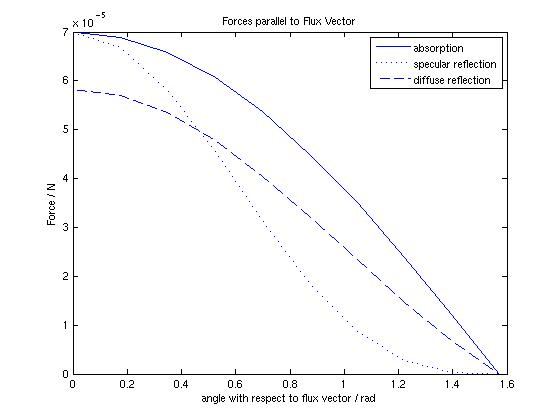
\includegraphics[width=180mm]{figs/Fsda/forces_parallel.jpg}
        \caption{The components of the absorption, specular, and diffuse forces
        parallel to the flux vector as a function of the angle between the flux
        vector and the surface normal}
        \label{fig:ivv_F_asd_values_par}
    \end{figure}

    \begin{figure}[!ht]
        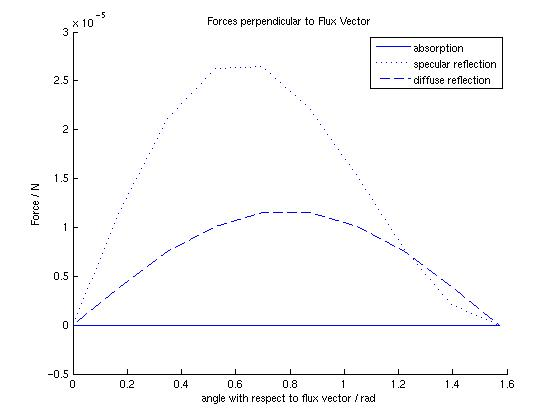
\includegraphics[width=180mm]{figs/Fsda/forces_perpendicular.jpg}
        \caption{The components of the absorption, specular, and diffuse forces
        perpendicular to the flux vector as a function of the angle between the
        flux vector and the surface normal}
        \label{fig:ivv_F_asd_values_perp}
    \end{figure}
  \end{description}

  \clearpage

\subsection{Verification of the Temperature Integration and Thermal
Emission Procedures}\label{test:temperature}

  This section is divided into two parts, one comparing the case of
  the vehicle without illumination --- for which an analytic solution
  exists --- and the second comparing the response of surfaces with different
  characteristics in the presence of illumination.

  \subsubsection{Verification of Thermal Processes without Illumination}
  \test{Thermal Processes - no illumination}
  \label{test:temperature_integration1}
  \begin{description}
  \item{Purpose:}\ \newline
    This test is to ensure that the Runge-Kutte plate-temperature integration
    process is functioning normally in the case of a vehicle cooling in the
    absence of incident radiation.
  \item{Requirements:}\ \newline
    Satisfactory conclusion of this test, along with test~\ref{test:temperature_integration2} satisfies requirements~\ref{reqt:functional_temperature} and~\ref{reqt:temperaturestructure}.

    Satisfactory conclusion of this test, along with the tests~\ref{test:temperature_integration2} and ~\ref{test:Fasd} satisfies requirement~\ref{reqt:functional_interaction}.
  \item{Procedure:}\ \newline
    The simulations used in this test are available at \textit{SIM\_2\_SHADOW\_CALC/RUN\_shadow\_cooling} (for the regular Surface Model surface) and at \textit{SIM\_2A\_SHADOW\_CALC/RUN\_shadow\_cooling} (for the default surface).
    For the Surface Model, a number of plates were monitored in a flux-free environment to observe
    their temperature variation with time, and the effect of that temperature
    variation on the variation of the emissive force with time.  Each plate had
    slightly different characteristics, allowing for the dependency on
    emissivity, plate area, and heat capacity to be investigated.  For the second simulation, a default surface was placed in the same environment.  In the
    absence of incident flux, an analytic solution exists for the temperature
    and the force, and this can be compared to the numerical solution.
  \item{Results:}
    \begin{enumerate}
    \item{Variation with time of force}\newline
      As expected, the absorption, diffuse, and specular forces were all zero
      for the duration of this simulation.
      The emission forces matched well with analytic predictions (see Figure~\ref{fig:forceanalytic}, and had the
      correct orientation.
    \item{Variation with time of temperature}\newline
      Simulation data matched very well to analytic solution.  On any scale
      longer than 3 timesteps, the graphs of analytical values and simulation
      values were indistinguishable, with a difference less than 0.05\%, and
      very much smaller than the observed changes in temperature.  See Figure~\ref{fig:temperatureanalytic}.
    \item{Variation with emissivity of the temporal evolution of temperature}\newline
      As the emissivity increases, the rate of change of temperature also
      increases, as expected.  For $\epsilon$=0, no temperature
      change was observed.
    \item{Variation with starting temperature of the temporal evolution of temperature}\newline
      With a lower starting temperature, a plate maintains a lower temperature
      throughout the simulation, but the temperature decreases more slowly.
      Temperature$\sim$time plots have identical shapes; shifting the curves along
      the x-axis to match temperature at some time results in matching
      temperatures for all (valid) time.
    \item{Variation with plate area of the temporal evolution of temperature}\newline
      A plate with a smaller surface area, but identical heat capacity shows a
      more gradual temperature drop.  There is no observable difference between
      plates for which the heat capacity is decreased proportionally with the
      area (e.g. smaller plate of the same material).
    \item{Variation with heat capacity of the temporal evolution of temperature}\newline
      A plate with a smaller heat capacity, but identical area shows a
      more rapid temperature drop.  There is no observable difference between
      plates for which the area is decreased proportionally with the heat
      capacity (e.g. smaller plate of the same material).
    \end{enumerate}

    \begin{figure}
         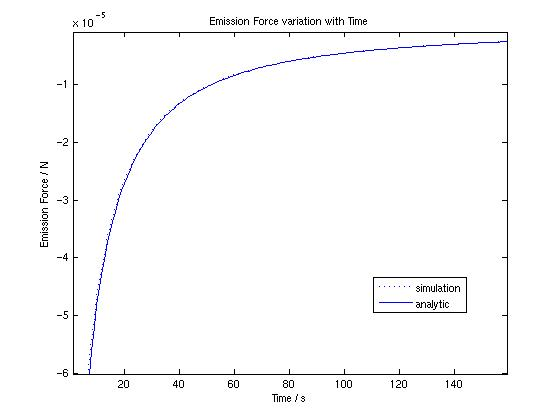
\includegraphics[width=180mm]{figs/Fe_int/force_analytic.jpg}
         \caption{Variation with time of force, showing the simulation data
         and analytic solution overlaying.}
         \label{fig:forceanalytic}
    \end{figure}
    \begin{figure}
         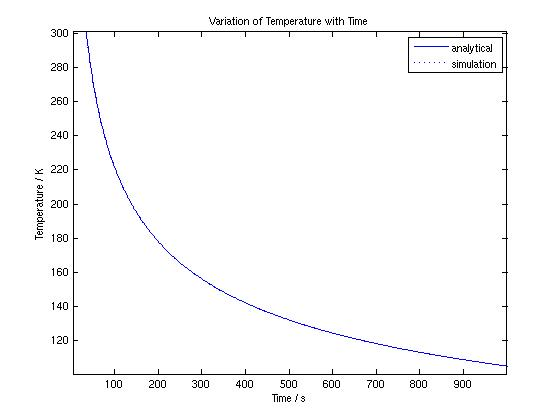
\includegraphics[width=180mm]{figs/Fe_int/temperature_analytic.jpg}
         \caption{Variation with time of temperature, showing the simulation data
         and analytic solution overlaying.}
         \label{fig:temperatureanalytic}
    \end{figure}

  \end{description}
  \clearpage

  \subsubsection{Verification of Thermal Processes with Illumination}
  \test{Thermal Processes - with illumination}
  \label{test:temperature_integration2}
  \begin{description}
  \item{Purpose:}\ \newline
    To verify that the temperature integration and thermal emission processes
    are functioning as expected when the vehicle is illuminated.
  \item{Requirements:}\ \newline
    Satisfactory conclusion of this test, along with test~\ref{test:temperature_integration1} satisfies requirements~\ref{reqt:functional_temperature} and~\ref{reqt:temperaturestructure}.

    Satisfactory conclusion of this test, along with the tests~\ref{test:temperature_integration1} and ~\ref{test:Fasd} satisfies requirement~\ref{reqt:functional_interaction}.
  \item{Procedure:}\ \newline
  The simulation used in this test is available at \textit{SIM\_2\_SHADOW\_CALC/RUN\_ten\_plates}.
    Ten identical plates were oriented at different angles to the flux
    vector, with the angle between the normal and the flux vector varying
    from 0 to 90 degrees.  All plates were started with a preliminary
    temperature of 270 K, and the simulation was allowed to run until all but
    one plate had approached their equilibrium temperature.  The force from each plate
    was monitored throughout the simulation.
  \item{Results:}\ \newline
    The equilibrium temperature is calculated from the energy balance equation
    \begin{equation}
      \phi (A\cos \theta )(1-\alpha )=\epsilon \sigma A{T_{\mathit{eq}}}^{4}
    \end{equation}

    where
    \begin{itemize}
      \item{}
        $\phi$ is the radiative flux,
      \item{}
        $\theta$ is the angle between the surface normal and the incident
        radiation vector,
      \item{}
        $\alpha$ is the albedo of the surface,
      \item{}
        $\epsilon$ is the emissivity of the surface,
      \item{}
        $\sigma$ is the Stefan-Boltzmann constant,
      \item{}
        A is the plate area, and
      \item{}
        $T_{\mathit{eq}}$ is the equilibrium temperature.
    \end{itemize}

    Using values of $\alpha =0.5$,  $\epsilon =0.5$, $\phi =
    1400~W~ m^{-2}$, and with $\theta$ varying from 0 to 90 degrees in 10 degree
    intervals, the equilibrium temperatures of the 10 plates are:

    396 K, 395 K, 390 K, 382 K, 371 K, 355 K, 333 K, 303 K, 256 K, and 0 K.

    Figure~\ref{fig:ivv_F_emission_Tint} shows the variation with time of the
    temperature of the 10 plates; the 9 plates that had closely approached equilibrium temperatures had
    final temperatures all within
    1\% of their analytical equilibrium temperature.

      \begin{figure}[!ht]
        \includegraphics[width=180mm]{figs/Fe_int/temperature-time.jpg}
        \caption{The variation of temperature with time over the 10 plates in
        the simulation.}
        \label{fig:ivv_F_emission_Tint}
      \end{figure}

    The final plate, with an equilibrium temperature of 0 K has a temperature
    variation that is decreasing at a rate consistent with expectations.

    The force due to emission should be directed opposite to the surface
    normal, and have magnitude equal to the ratio of power emission to speed of
    light, producing equilibrium values of 47, 46, 44, 40, 36, 30, 23, 16, 8,
    and 0  ${\mu}$N.

    Figure~\ref{fig:ivv_F_emission_10plate} shows the variation with
    time of the force due to emission, confirming the analytic
    values.
    \begin{figure}[!ht]
        \includegraphics[width=180mm]{figs/Fe_int/force_emission10plate.jpg}
        \caption{The variation with time of force, over the 10 plates in
        the simulation.}
        \label{fig:ivv_F_emission_10plate}
      \end{figure}
  \clearpage
  \end{description}
\clearpage

\subsection{Verification of the Flux Calculations}\label{sec:verifflux}

This section is divided into two parts:  the first considers a
vehicle in Earth's shadow at several locations along the extension
of the Sun-Earth
vector, the second considers a vehicle moving perpendicular to the
Sun-Earth vector, passing through Earth's shadow.

  \subsubsection{Eclipse calculations along the extension of the Sun-Earth vector}
    \test{Verification of the eclipse calculation for an object
      moving along the Sun-planet axis through the region of annular eclipse}
    \label{test:eclipse_annular}
    \begin{description}
      \item{Purpose:}\ \newline
        The purpose of this simulation is to confirm that the code
        correctly identifies and calculates the extent of shadowing by an
        intervening body.
      \item{Requirements:}\ \newline
        The results of this test, together with the results
        from~\ref{test:eclipse_transverse}, together satisfy
        requirement~\ref{reqt:functional_eclipse}.
      \item{Procedure:}\ \newline

The simulation used in this test is available at \textit{SIM\_2\_SHADOW\_CALC/RUN\_annular\_eclipse}.
        The vehicle was placed at various locations along the dotted line shown
        in figure~\ref{fig:ivv_annular_eclipse_layout}.

        \begin{figure}[!ht]
          \includegraphics[width=180mm]{figs/eclipse/annular_eclipse_layout.jpg}
          \caption{The location of the vehicle, with respect to Earth and Sun,
                 during the simulation.}
          \label{fig:ivv_annular_eclipse_layout}
        \end{figure}
        Two runs were made:
        \begin{enumerate}
          \item{} the first used the cylindrical shadow model,
          \item{} the second used the conical shadow model.
        \end{enumerate}
          The value of the flux vector was evaluated at several
          locations for each run.
      \item{Results:}\ \newline
        Both runs produced results entirely in line with expectations.
        \begin{enumerate}
          \item{}
            For the first run (cylindrical shadow), there was no illumination at any location on
            the line.
          \item{}
            For the second run (conical shadow), there was no illumination while the vehicle
            was inside the cone representing totality.
            At larger distances, the magnitude of the flux increased as a
            greater percentage of the solar disk became visible; at very
            large distances from Earth ($>10^{10}$  m), the flux magnitude
            decreased with distance due to the inverse-square nature of
            the flux magnitude and the fact that the fraction of the solar
            disk that is exposed changes only very slowly at these distances.
            The data matched the theoretical predictions very closely.
            \begin{figure}[!ht]
       \includegraphics[width=180mm]{figs/eclipse/flux-radial_distance.jpg}
              \caption{The flux of the vehicle as a function of distance
                from Earth on the Sun-Earth vector.  The raw flux represents
                the solar flux without shadowing.  The predicted flux
                represents the analytic function
                for flux with Earth shadowing included.  Data points from the
                simulation are shown as circles.}
              \label{fig:ivv_flux_radial_distance}
            \end{figure}
        \end{enumerate}
     \end{description}
\clearpage

  \subsubsection{Eclipse calculations perpendicular to the extension of the
     Sun-Earth vector}
  \test{Verification of the eclipse calculation for an object
    moving across the region of total eclipse}
  \label{test:eclipse_transverse}
  \begin{description}
    \item{Purpose:}\newline
      The purpose of this simulation is to confirm that the code
      correctly identifies and calculates the extent of shadowing by an
      intervening body.
    \item{Requirements:}\newline
        The results of this test satisfy
        requirement~\ref{reqt:functional_flux}, and together with the results
        from~\ref{test:eclipse_annular}, satisfy
        requirement~\ref{reqt:functional_eclipse}.
    \item{Procedure:}\newline

The simulation used in this test is available at \textit{SIM\_2\_SHADOW\_CALC/RUN\_transverse\_shadow}.
      Two different techniques were used to investigate the
      response to the position within the shadow of the planet.
      \begin{enumerate}
        \item{}
        A series of runs was made with the vehicle traversing the shadow,
        perpendicular to the Sun{}-Earth vector at a selection of values of
        $r_{\mathit{par}}$, the component of the Earth-vehicle vector parallel to
        the Sun-Earth vector, as shown in
        Figure~\ref{fig:ivv_transverse_eclipse_layout}.
        The simulation included in the \JEODid\ release corresponds to line number 4 in this description.  With an Earth-vehicle distance of $1.35 \times 10^9 m$, this corresponds to the apex of the cone representing totality.  Line number 1 in this description is actually located at a distance of $1.35 \times 10^4 m$ from the center of Earth.  This value is well within the planet; values closer to the planet center had complicating issues associated with Earth moving on its orbit during the simulation in such a way that the position of the vehicle was closer to Sun than was Earth.
        \begin{figure}[!ht]
          \includegraphics[width=180mm]{figs/eclipse/drawings1_te.jpg}
          \caption{The 6 paths of the vehicle across Earth's shadow}
          \label{fig:ivv_transverse_eclipse_layout}
        \end{figure}

        \item{}
        Another run was made in which the inertial position of the
        vehicle was held fixed with respect to Earth, and the ephemeris allowed to evolve.
        Starting with the vehicle in the conical shadow, it gradually moved
        into full sunlight as the earth moved around its orbit, as shown in
        Figure~\ref{fig:ivv_transverse_eclipse_layout2}.


        \begin{figure}[!ht]
          \includegraphics[width=80mm]{figs/eclipse/drawings2_te.jpg}
          \caption{The position of the vehicle with respect to Sun as it transits
            Earth's shadow.}
          \label{fig:ivv_transverse_eclipse_layout2}
        \end{figure}
      \end{enumerate}

    \item{Results:}\newline
    \begin{enumerate}

      \item{}
      In the first run (vehicle passes through Earth shadow), the Sun-vehicle vector changes in both direction and
      magnitude, thus
      affecting the flux unit vector (flux\_hat), the magnitude of the flux
      vector, and each individual component of the flux vector; these changes
      were consistent with theory.

    The six lines in Figure~\ref{fig:ivv_flux_transverse_eclipse}
    each represent the magnitude of the force
    experienced by a vehicle as it traverses Earth's shadow.  Each line
    represents a different value of $r_{\mathit{par}}$ and is
    shown as a function of $r_{\mathit{perp}}$, the component of the
    Earth-vehicle vector that is perpendicular to the Sun-Earth vector.

    For passes that were sufficiently close to Earth that the vehicle passed through the region of totality (i.e. passes 1-3, with pass 4 satisfying this requirement only momentarily), we see the effects of both umbral and penumbral shadowing.  The penumbral (partial shadowing)
    region is indicated by a sloping line; the umbral (total shadowing) region
    is indicated by a flat line and zero force.

    The first line (corresponding to a vehicle passing close to the center of Earth) shows no penumbral region, and an umbral region equal in
    size to Earth.  Getting farther from Sun, the extent of the penumbral
		region grows, and that of
    the umbral region shrinks until it disappears by the fourth line, which is the limit of total eclipse.  Farther yet from Earth, passes 5 and 6 represent annular eclipses, with the angular size of Earth now
		smaller than that of the sun.  Annular eclipses do not have umbral regions; instead the flux should fall until the intervening body is completely within the solar disk, then stay constant as the intervening body traverses the solar disk, then rise again as it leaves the disk.  Pass 6 in particular shows the annular eclipse lasting for some distance at
    constant illumination.  Also, evident in the wings of the first three lines,
    beyond the points of total illumination, is the gradual decrease in
    illumination due to increased distance from Sun.

    \begin{figure}[!ht]
      \includegraphics[width=180mm]{figs/eclipse/force_partial_eclipse.jpg}
      \caption{The magnitude of the radiative force as a function of
      $r_{\mathit{perp}}$ for different values of $r_{\mathit{par}}$}
      \label{fig:ivv_flux_transverse_eclipse}
    \end{figure}

    \item{}
      The second simulation (shadow moves with respect to a fixed-orientation of Earth and vehicle) demonstrated very similar results, with
      almost-negligible changes in the Sun-vehicle distance, and
      hence in the raw flux magnitude throughout the simulation.
    \end{enumerate}
  \end{description}
\clearpage


\subsubsection{Confirmation of eclipsing bodies}
\inspection{Vehicle can be shadowed by any intervening body.}\ \newline
\label{inspect:eclipsingbody}
The functionality to calculate the effect of an eclipsing body is demonstrated in tests~\vref{test:eclipse_annular} and \vref{test:eclipse_transverse}.  The flexibility to include shadowing of more than one body is found in \textit{RadiationSource::calculate\_flux}, although this is not complete;  where two intervening bodies overlap, the code will calculate the fractional part of the disk that is visible behind each (e.g. 90\% and 80\%) and multiply these together (72\%).  If the two bodies are blocking the same part of the disk, this is an invalid number.  For a fully correct implementation, the ``shadowing'' of third-bodies by third-bodies also needs to be considered.  Nevertheless, the requirement is for this functionality to be available as an extension, and in that sense, this inspection satisfies requirement~\ref{reqt:eclipsingbody}.


%\section{Validation}
%%%%%%%%%%%%%%%%%%%%%%%%%%%%%%%%%%%%%%%%%%%%%%%%%%%%%%%%%%%%%%%%%%%%%%%%%%%%%%%
%
% Purpose:  Validation part of V&V for the RadiationPressure model
%
%
%%%%%%%%%%%%%%%%%%%%%%%%%%%%%%%%%%%%%%%%%%%%%%%%%%%%%%%%%%%%%%%%%%%%%%%%%%%%%%%

\section{Validation}

%%% code imported from old template structure
%\test{<Title>}\label{test:<label>}
%\begin{description}
%\item[Purpose:] \ \newline
%<description>
%\item[Requirements:] \ \newline
%By passing this test, the universal time module
%partially satisfies requirement~\ref{reqt:<label1>} and
%completely satisfies requirement~\ref{reqt:<label2>}.
%\item[Procedure:]\ \newline
%<procedure>
%\item[Results:]\ \newline
%<results>
%\end{description}



\subsection{Validation of Flux-Vehicle Interaction-Model Principles}
\test{Flux-Vehicle Interaction Model Principles}
  \label{test:flux_vehicle_interaction}
  \begin{description}
    \item[Purpose:] \ \newline
      The purpose of this test is to validate that radiation-interaction
      can be modeled to reasonable accuracy by a combination of specular
      reflection, diffuse reflection, absorption, and emission.
    \item[Requirements:] \ \newline
      By passing this test, the model satisfies
      requirement~\ref{reqt:functional_interaction}.
    \item[Procedure:]\ \newline
      A number of test surfaces were run.
      Figure~\ref{fig:ivv_surface_profiles} shows the reflections
      for a series of four surfaces of progressively increasing roughness
      (and hence higher $\delta $, the weighting towards diffuse reflection).
      Each of these surfaces was tested with 3 different
      albedos, across a range of incident angles.  For each
      incident angle, 10\textsuperscript{6} ``photons'' were
      ``fired'' at the surface and the subsequent reflection or absorption
      recorded (see Figure \ref{fig:ivv_surface_profiles} for reflection
			characteristics).

      \begin{figure}[!ht]
        \includegraphics[width=95mm]{figs/sda/reflection1_sda.jpg}
        \includegraphics[width=95mm]{figs/sda/reflection2_sda.jpg}
        \includegraphics[width=95mm]{figs/sda/reflection3_sda.jpg}
        \includegraphics[width=95mm]{figs/sda/reflection4_sda.jpg}
        \includegraphics[width=105mm,height=70mm]{figs/blank.jpg}
        \includegraphics[width=75mm]{figs/sda/reflection5_sda.jpg}
        \caption{Reflection characteristics from four surfaces}
        \label{fig:ivv_surface_profiles}
      \end{figure}

      The vectors associated with photon reflections were averaged and
      compared to the theoretical average for thin-film
      interactions, equation \vref{eqn:s_hat_average}.

      \begin{equation*}
           \langle \hat{s}\rangle =\left[\begin{matrix}-0.5\;\sin \phi
           \;\left(1+e^{-\frac{1}{c}}\right)\\0\\\cos \phi
           \;e^{-\frac{1}{c}}\end{matrix}\right]
        \end{equation*}


      This theoretical value includes the possibility that a photon
      could be reflected downward as its terminal state, while the
      simulation took downward reflected photons and operated on them
      again until they were either absorbed by the surface, or
      reflected away from the surface.

 			In this representation, the x-axis is the negative of the projection
			of the incident radiation onto the surface;
			the z-axis is perpendicular to the surface, pointing outward
			the y-axis is parallel to the surface, and completes the right-hand
			coordinate system; \textit{c} represents the ``smoothness'' of the surface.

      The cumulative vector force calculated from the
      interactions of all photons for any given angle and surface was
      then compared with a best-fit bulk approximation that assigned some
      fraction of the incident photons to specular reflection, some to
      diffuse reflection, and some to absorption and subsequent
      emission.
    \clearpage

    \item[Results:]\ \newline
     The results section is divided into two parts: a comparison of the
     values for the unit-vector associated with reflection, and a
     comparison of the values for the force.

     \subsubsection{Unit-vector Comparisons}


      The average unit-reflection-vector, $\langle \hat{s}\rangle$, was
      calculated from the numerical simulation and compared to the analytic
      value given above.  Figure~\ref{fig:ivv_sda_s_vector} shows the comparison
      between the numerical and analytical value for each of the three
      components of $\langle \hat{s}\rangle$ for surface \#1.

      \begin{figure}[!ht]
        \includegraphics[width=95mm]{figs/sda/s_x_smooth.jpg}
        \includegraphics[width=95mm]{figs/sda/s_y_smooth.jpg}
        \includegraphics[width=95mm]{figs/sda/s_z_smooth.jpg}
        \caption{Analytical and numerical mean values for components of
                 the reflection vector from a smooth surface as a
                 function of incident angle}
        \label{fig:ivv_sda_s_vector}
      \end{figure}

      Figures~\ref{fig:ivv_sda_s_vector_diffs_x},
      ~\ref{fig:ivv_sda_s_vector_diffs_y},
      and~\ref{fig:ivv_sda_s_vector_diffs_z} show the differences
      along each axis for each of the four surfaces shown in
      Figure~\ref{fig:ivv_surface_profiles}.

      \begin{figure}[!ht]
        \includegraphics[width=95mm]{figs/sda/unit_vec_diff__x_smooth.jpg}
        \includegraphics[width=95mm]{figs/sda/unit_vec_diff__x__gloss.jpg}
        \includegraphics[width=95mm]{figs/sda/unit_vec_diff__x__matte.jpg}
        \includegraphics[width=95mm]{figs/sda/unit_vec_diff__x__rough.jpg}
        \caption{Differences between the analytic and numeric x-component of
                 $\langle \hat{s}\rangle$ for each of the 4
                 surface-profiles.}
        \label{fig:ivv_sda_s_vector_diffs_x}
      \end{figure}

      \begin{figure}[!ht]
        \includegraphics[width=95mm]{figs/sda/unit_vec_diff__y_smooth.jpg}
        \includegraphics[width=95mm]{figs/sda/unit_vec_diff__y__gloss.jpg}
        \includegraphics[width=95mm]{figs/sda/unit_vec_diff__y__matte.jpg}
        \includegraphics[width=95mm]{figs/sda/unit_vec_diff__y__rough.jpg}
        \caption{Differences between the analytic and numeric y-component of
                 $\langle \hat{s}\rangle$ for each of the 4
                 surface-profiles.}
        \label{fig:ivv_sda_s_vector_diffs_y}
      \end{figure}

      \begin{figure}[!ht]
        \includegraphics[width=95mm]{figs/sda/unit_vec_diff__z_smooth.jpg}
        \includegraphics[width=95mm]{figs/sda/unit_vec_diff__z__gloss.jpg}
        \includegraphics[width=95mm]{figs/sda/unit_vec_diff__z__matte.jpg}
        \includegraphics[width=95mm]{figs/sda/unit_vec_diff__z__rough.jpg}
        \caption{Differences between the analytic and numeric z-component of
                 $\langle \hat{s}\rangle$ for each of the 4
                 surface-profiles.}
        \label{fig:ivv_sda_s_vector_diffs_z}
      \end{figure}

      \clearpage

     \subsection{Force Comparisons}
      For each angle of incidence, the total force calculated by
      each of the two models can be expressed as:
      \begin{enumerate}
        \item{}Numerical Model
          \begin{equation}
            {\vec{F}}_{\mathit{num}}=\sum _{i=1}^{N}\vec{\mathit{dF}}_{i}
            \label{eqn:ivv_fvi_force_numerical}
          \end{equation}

          where \newline
          \begin{itemize}
            \item{}
              $\vec{\mathit{dF}}_{i}=
                \begin{cases}
                  f_{\gamma }\left(-\hat{p}-\hat{s}_{i}\right) &
                    \mathit{photon~ is~ reflected}\\
                  f_{\gamma }\left(-\hat{p}-\frac{2}{3}\hat{k}\right) &
                    \mathit{photon~ is~
                    absorbed~and~re-emitted,~or~reflected~diffusely}
                \end{cases}$
            \item{}
              $\hat{p}$,$\hat{s}$, and $\hat{k}$ are unit vectors for the
              incident radiation, specular reflection, and surface-normal
              vectors (Note:  $\hat{p}$ is directed \it against \rm the flux
              vector, away from the surface).
            \item{}
              $f_{\gamma }$ represents the ``force'' associated with the
              momentum of each incident photon per unit time.
            \item{}
              \textit{N} represents the number of ``photons'' being
              used.
          \end{itemize}

        \item{}Simplifying Model
          \begin{equation}
            {\vec{F}}_{\mathit{model}}=Nf_{\gamma }\left(-\hat{p}-\alpha
            (1-\delta)\hat{s}-\frac{2}{3}(1-\alpha (1-\delta ))\hat{k}\right)
            \label{eqn:ivv_fvi_force_simple}
          \end{equation}

          where  $\alpha $ and  $\delta $ represent the fraction of incident
          light that is reflected, and the fraction of the reflected
          light that is reflected diffusely.

      \end{enumerate}
      Equation~\ref{eqn:ivv_fvi_force_numerical} is evaluated
      for each angle of incidence, for each surface by calculating the force
      from each photon, and summing to provide the total force in
      each direction.

      For any given surface, the force is calculated for a number of incident
      angles, then the values  $\alpha $ and  $\delta $,  that provide the
      best fit ---  across all of those angles --- between
      equations ~\ref{eqn:ivv_fvi_force_numerical}
      and ~\ref{eqn:ivv_fvi_force_simple}, are
      determined.

      First the difference, \it per photon, \rm between
      equations~\ref{eqn:ivv_fvi_force_numerical}
      and~\ref{eqn:ivv_fvi_force_simple}
      is calculated for some angle of incidence ,  $\phi _{i} $ :

      \begin{equation}
        (\vec{{\Delta F}}_{\phi _{i} })=
        \frac{{\vec{F}}_{\mathit{num}}-{\vec{F}}_{\mathit{model}}}{N}
      \end{equation}

      The RMS value is used for determining ``best fit''.

      \begin{equation}
        \Delta F_{\mathit{RMS}}=\sqrt{\frac{1}{n}\sum _{i=1}^{n}|\vec{{\Delta
        F}}_{\phi _{i}}|^{2}}
      \end{equation}

      where \it n \rm represents the number of angles of incidence
      used in the numerical simulation.

      The contribution to this value from each axis are
      also calculated for analysis.

      \begin{equation}
        \Delta F_{x}=\sqrt{\frac{1}{n}\sum _{i=1}^{n}\left((\vec{{\Delta
        F}}_{\phi _{i}})\cdot \hat{i}\right)^{2}}
      \end{equation}

      \begin{equation}
        \Delta F_{y}=\sqrt{\frac{1}{n}\sum _{i=1}^{n}\left((\vec{{\Delta
        F}}_{\phi _{i}})\cdot \hat{j}\right)^{2}}
      \end{equation}

      \begin{equation}
        \Delta F_{z}=\sqrt{\frac{1}{n}\sum _{i=1}^{n}\left((\vec{{\Delta
        F}}_{\phi _{i}})\cdot \hat{k}\right)^{2}}
      \end{equation}


      Values of $\alpha $ and  $\delta $ which minimize  $\Delta
      F_{\mathit{RMS}}$ are now determined, and those values used in
      equation~\ref{eqn:ivv_fvi_force_simple} to obtain a ``best'' estimate of
      the variation with incident
      angle of the force. The comparison of the numerical simulation to the
      best fit is shown in figures~\ref{fig:ivv_sda_f_vector_diffs_x},
     ~\ref{fig:ivv_sda_f_vector_diffs_y}, and
     ~\ref{fig:ivv_sda_f_vector_diffs_z}.
      Note that in places, the best
      fit line is wholly above or below the data; this is because the data are
      showing 1 dimension at a time, whereas the best fit line is based on
      all dimensions together.

      \begin{figure}[!ht]
        \includegraphics[width=95mm]{figs/sda/F__x_diff_smooth.jpg}
        \includegraphics[width=95mm]{figs/sda/F__x_diff__gloss.jpg}
        \includegraphics[width=95mm]{figs/sda/F__x_diff__matte.jpg}
        \includegraphics[width=95mm]{figs/sda/F__x_diff__rough.jpg}
        \caption{Mean values for the analytic and numeric x-component of
                the interaction force for each of the 4
                surface-profiles.}
        \label{fig:ivv_sda_f_vector_diffs_x}
      \end{figure}

      \begin{figure}[!ht]
        \includegraphics[width=95mm]{figs/sda/F__y_diff_smooth.jpg}
        \includegraphics[width=95mm]{figs/sda/F__y_diff__gloss.jpg}
        \includegraphics[width=95mm]{figs/sda/F__y_diff__matte.jpg}
        \includegraphics[width=95mm]{figs/sda/F__y_diff__rough.jpg}
        \caption{Mean values for the analytic and numeric y-component of
                the interaction force for each of the 4
                surface-profiles.}
        \label{fig:ivv_sda_f_vector_diffs_y}
      \end{figure}

      \begin{figure}[!ht]
        \includegraphics[width=95mm]{figs/sda/F__z_diff_smooth.jpg}
        \includegraphics[width=95mm]{figs/sda/F__z_diff__gloss.jpg}
        \includegraphics[width=95mm]{figs/sda/F__z_diff__matte.jpg}
        \includegraphics[width=95mm]{figs/sda/F__z_diff__rough.jpg}
        \caption{Mean values for the analytic and numeric z-component of
                the interaction force for each of the 4
                surface-profiles.}
        \label{fig:ivv_sda_f_vector_diffs_z}
      \end{figure}

      Notice that for all surfaces the behavior in the y-direction
      is small and unpredictable.
      For the smooth surface (surface \#1),
      the x{}- and z{}- components of the force behave
      as expected. In the x{}-direction, a highly reflective surface should
      produce no force, while a highly absorbent surface should absorb all of
      the momentum from the incident radiation, which varies as $\sin \phi$.
      In the z{}-direction, the highly reflective surface should
      experience a force of magnitude  $\cos \phi $ from each of incident and
      reflected radiation components, resulting in a curve that decreases from
      2 at
      $\phi =0$ to 0 at  $\phi =90$ degrees; the highly absorbent surface will
      experience the  $\cos \phi $ force from the incident radiation, and a
      force with magnitude 2/3 from the re{}-emitted radiation, causing the
      curve to fall from 1.67 to 0.67. The forces in the y{}-direction
      should be generally small compared with those in the x{}- and
      z{}-direction. These features are all observed. In all cases,
      values of $\alpha $ and  $\delta $ were found that provided a close fit
      between the numerical data and the simplified expression given in
      equation~\ref{eqn:ivv_fvi_force_simple}.

      \clearpage

      On closer inspection, under certain circumstances, the best fit of
      $\alpha $ and  $\delta $ to the data did not seem sensible. To
      investigate the degree to which the determination of the albedo and
      diffuse parameters are critical, plots have been generated showing the
      deviations  $\Delta F_{\mathit{RMS}}$ , $\Delta F_{x}$ and $\Delta
      F_{z}$ as functions of  $\alpha $ and  $\delta $ . An example of this
      may be seen on the error associated with a matte surface at medium
      albedo, which should have mid{}-range values for both  $\alpha $ and
      $\delta $ . From Figure~\ref{fig:ivv_sda_alpha_delta_F}, it is clear that
      appropriate values of
      0.6 and 0.4 respectively find the region of minimum error. However,
      the algorithmic search would not be able to distinguish between this,
      and values of 1.0 and 0.6 for  $\alpha $ and  $\delta $, which would
      be characteristic of a highly unusual surface that is both highly
      reflective and very rough.

      These data, presented in Figures~\ref{fig:ivv_sda_alpha_delta_F},
     ~\ref{fig:ivv_sda_alpha_delta_Fx}, and~\ref{fig:ivv_sda_alpha_delta_Fz},
      confirmed that ``sensible''
      values existed with very similar error even in those cases where the
      algorithmic search for lowest error produced unusual results. It is
      also apparent that there are a number of solutions of approximately
      equivalent merit, and that the determination of  $\alpha $ and  $\delta
      $ is probably not critical to better than 1 part in 10, and certainly
      not beyond 1 part in 100. At low albedo particularly, there is very little
      difference between the four surfaces, and making significant investment in a
      precise determination of $\alpha $ and  $\delta $ is futile.

      For
      reference on these figures, recall that the force{}-error is expressed
      \textit{per photon}, and that an error of value 1 is
      equivalent to the effect of the total incident radiation if it were all
      absorbed.
      The largest possible force-value on this scale is 2, which
      occurs in the vertical direction when $\phi =0$,
      and $\alpha =1$ on a perfectly smooth surface.

      This observation is further supported by data presented in
      section~\ref{test:plate_model},
      Figures~\ref{fig:ivv_platemod_fig1} to~\ref{fig:ivv_platemod_specdiff}.
      While the two
      types of reflection produce Force-time graphs with very different
      patterns, the integration of those graphs yields impulses that are quite
      similar.

  \begin{figure}[!ht]
  \leftskip=-20mm
  \begin{minipage}[t]{200mm}\centering
    \includegraphics[width=65mm]{figs/sda/F_error_albedo_high_surf_smooth.jpg}
    \includegraphics[width=65mm]{figs/sda/F_error_albedo__med_surf_smooth.jpg}
    \includegraphics[width=65mm]{figs/sda/F_error_albedo__low_surf_smooth.jpg}
    \includegraphics[width=65mm]{figs/sda/F_error_albedo_high_surf__gloss.jpg}
    \includegraphics[width=65mm]{figs/sda/F_error_albedo__med_surf__gloss.jpg}
    \includegraphics[width=65mm]{figs/sda/F_error_albedo__low_surf__gloss.jpg}
    \includegraphics[width=65mm]{figs/sda/F_error_albedo_high_surf__matte.jpg}
    \includegraphics[width=65mm]{figs/sda/F_error_albedo__med_surf__matte.jpg}
    \includegraphics[width=65mm]{figs/sda/F_error_albedo__low_surf__matte.jpg}
    \includegraphics[width=65mm]{figs/sda/F_error_albedo_high_surf__rough.jpg}
    \includegraphics[width=65mm]{figs/sda/F_error_albedo__med_surf__rough.jpg}
    \includegraphics[width=65mm]{figs/sda/F_error_albedo__low_surf__rough.jpg}
  \end{minipage}
    \caption{Differences in the value of the magnitude of the model force, comparing the numerical simulation
    to the simplified model, as a function of $\alpha$ and $\delta$,
    presented in matrix formation with rows representing (from top) surface
    1-4, and columns representing (from left) high to low albedo.}
    \label{fig:ivv_sda_alpha_delta_F}
  \end{figure}

  \begin{figure}[!ht]
  \leftskip=-20mm
  \begin{minipage}[t]{200mm}\centering
    \includegraphics[width=65mm]{figs/sda/F_x_error_albedo_high_surf_smooth.jpg}
    \includegraphics[width=65mm]{figs/sda/F_x_error_albedo__med_surf_smooth.jpg}
    \includegraphics[width=65mm]{figs/sda/F_x_error_albedo__low_surf_smooth.jpg}
    \includegraphics[width=65mm]{figs/sda/F_x_error_albedo_high_surf__gloss.jpg}
    \includegraphics[width=65mm]{figs/sda/F_x_error_albedo__med_surf__gloss.jpg}
    \includegraphics[width=65mm]{figs/sda/F_x_error_albedo__low_surf__gloss.jpg}
    \includegraphics[width=65mm]{figs/sda/F_x_error_albedo_high_surf__matte.jpg}
    \includegraphics[width=65mm]{figs/sda/F_x_error_albedo__med_surf__matte.jpg}
    \includegraphics[width=65mm]{figs/sda/F_x_error_albedo__low_surf__matte.jpg}
    \includegraphics[width=65mm]{figs/sda/F_x_error_albedo_high_surf__rough.jpg}
    \includegraphics[width=65mm]{figs/sda/F_x_error_albedo__med_surf__rough.jpg}
    \includegraphics[width=65mm]{figs/sda/F_x_error_albedo__low_surf__rough.jpg}
  \end{minipage}
    \caption{Differences in the value of the x-component of the model force, comparing the
    numerical simulation to
    the simplified model, as a function of $\alpha$ and $\delta$,
    presented in matrix formation with rows representing (from top) surface
    1-4, and columns representing (from left) high to low albedo.}
    \label{fig:ivv_sda_alpha_delta_Fx}
  \end{figure}
  \begin{figure}[!ht]
  \leftskip=-20mm
  \begin{minipage}[t]{200mm}\centering
    \includegraphics[width=65mm]{figs/sda/F_z_error_albedo_high_surf_smooth.jpg}
    \includegraphics[width=65mm]{figs/sda/F_z_error_albedo__med_surf_smooth.jpg}
    \includegraphics[width=65mm]{figs/sda/F_z_error_albedo__low_surf_smooth.jpg}
    \includegraphics[width=65mm]{figs/sda/F_z_error_albedo_high_surf__gloss.jpg}
    \includegraphics[width=65mm]{figs/sda/F_z_error_albedo__med_surf__gloss.jpg}
    \includegraphics[width=65mm]{figs/sda/F_z_error_albedo__low_surf__gloss.jpg}
    \includegraphics[width=65mm]{figs/sda/F_z_error_albedo_high_surf__matte.jpg}
    \includegraphics[width=65mm]{figs/sda/F_z_error_albedo__med_surf__matte.jpg}
    \includegraphics[width=65mm]{figs/sda/F_z_error_albedo__low_surf__matte.jpg}
    \includegraphics[width=65mm]{figs/sda/F_z_error_albedo_high_surf__rough.jpg}
    \includegraphics[width=65mm]{figs/sda/F_z_error_albedo__med_surf__rough.jpg}
    \includegraphics[width=65mm]{figs/sda/F_z_error_albedo__low_surf__rough.jpg}
  \end{minipage}
    \caption{Differences in the value of the z-component of the model force, comparing the
    numerical simulation to
    the simplified model, as a function of $\alpha$ and $\delta$,
    presented in matrix formation with rows representing (from top) surface
    1-4, and columns representing (from left) high to low albedo.}
    \label{fig:ivv_sda_alpha_delta_Fz}
  \end{figure}
      Of interest, there is a trend that as the surface gets rougher, $\alpha
      $ gets smaller and/or  $\delta $ gets larger.  This is expected behavior; as the surface gets rougher, more photons will be reflected ``down'' into the surface and be absorbed, reducing the albedo, those photons that are reflected upward are going to be more scattered, appearing as diffuse reflection more than specular reflection.
      For all four surfaces, the albedo settings (low, med, or
      high) are assigned by the value of the albedo of each
      microscopic plate.

  \end{description}

  \clearpage

\subsection{Validation of the Plate Model Assumptions}
\label{sec:platemodelvalid}
\test{Validation of the Plate Model Assumptions}
  \label{test:plate_model}
  \begin{description}
   \item{Purpose:}\newline
    To validate that, for the purposes of radiation
    pressure calculations, curved surfaces can be
    approximated by crude, gross-feature-only, flat plate
    models, and to assess the degree to which doing so
    introduces error into the system.

   \item{Procedure:}\newline
    The response of a square cuboid --- of side \it s \rm and length \it L
    \rm --- to a radiation field is compared
    to that of a cylinder of comparable dimensions, with the
    cuboid representing the flat-plate approximation to the
    cylinder.  The two objects were rotated in a constant radiation
    field with the long-axis perpendicular to the flux vector, as shown in
    figure~\ref{fig:ivv_isotherm_fig1}.

    This test was conducted using the \JEODid\ algorithms ported into MATLAB, while test \vref{test:sim4} compares the difference directly between the spherical default surface, and a cubic flat-plate surface.

    \begin{figure}[!ht]
      \begin{center}
      \includegraphics[width=150mm]{figs/isoth_app/iso_app_figs1.jpg}
      \end{center}
      \caption{Orientation of the cylinder and cuboid.}
      \label{fig:ivv_isotherm_fig1}
    \end{figure}

    The effects from the ends of the objects were ignored, which is
    essentially equivalent to assuming the objects to be long and thin.
    Rotation angles
    are measured counterclockwise from the lowest point on the
    object, as shown in figure~\ref{fig:ivv_isotherm_fig4}.

    \begin{figure}[!ht]
      \begin{center}
      \includegraphics[width=70mm]{figs/isoth_app/iso_app_figs4.jpg}
      \end{center}
      \caption{Definition of angle $\theta$.}
      \label{fig:ivv_isotherm_fig4}
    \end{figure}

    The cuboid starts `sitting' on one face, as shown
    in figure~\ref{fig:ivv_plate_model_fig1}.
    \begin{figure}[!ht]
      \begin{center}
      \includegraphics[width=90mm]{figs/cyl_cub_comp/cyl_cub_fig1.jpg}
      \end{center}
      \caption{Orientation of the cylinder and cuboid.}
      \label{fig:ivv_plate_model_fig1}
    \end{figure}

    The two objects were configured to allow for two extremes of temperature
    structures:
    \begin{enumerate}
     \item{}The temperature was uniform across the object (isothermal
     approximation).
     \item{}The temperature was spatially variable, with plates assumed to be
       thermally isolated for maximum temperature differential.  For this, the
       cylinder was configured to comprise a large collection of thin strips,
       running the length of the cylinder.
    \end{enumerate}

    Data are taken from the steady states of the two objects for
    each configuration (i.e. after initial transients have died away, the variability is due entirely to the rotation, and the temperature -- and therefore the force -- associated with each plate can be expressed as a function of $\theta$ only, with no other dependency on time).

    Finally, the dimensions of the cuboid were adjusted to investigate whether
    it was more important to have equivalent surface area, or equivalent
    enclosed volume as an approximation to the cylinder.

   \item{Mathematical development} \ \newline
     This section develops the equations used in these tests.

     \begin{enumerate}
     \item{Cuboid}
       \begin{enumerate}
         \item{Absorption:}\ \newline
           The rate at which energy is absorbed is the product of the flux
           vector, the projected area, and the absorptivity (equal to 1-albedo).
           The force, or momentum flux, is related to the energy flux by the
           speed of light.  The
           absorption will only produce a force in the direction of the incident
           radiation.  It will not be a constant, as the cuboid projects
           different cross section as it rotates.
           \begin{figure}[!ht]
             \begin{center}
             \includegraphics[width=90mm]{figs/isoth_app/iso_app_figs3.jpg}
             \end{center}
             \caption{The surface area projected perpendicular to the
                illumination vector.}
             \label{fig:ivv_isotherm_fig3}
           \end{figure}

           Incident flux falls on two projected areas, one of area
           $sL\sin \theta $ , and another of area $sL\cos \theta $ ,

           \begin{equation}
             \vec {F} = \left( \frac {1-\alpha}{c} \right)
             \phi s L (\sin \theta + \cos \theta) \hat {i}
           \end{equation}
          \item{Specular Reflection:}\ \newline
            Incident flux falls on the same two surfaces, where some fraction
            $\alpha $ is reflected, ($\alpha(1-\delta)$ is reflected
            specularly).  There are two force ``components'', one from
            `stopping' the incident radiation (in direction of radiation
            vector), and one `recoiling' from the reflected radiation (in
            direction opposite the radiation vector).  Use $\hat{r}_{i}$ to
            represent the direction of (specularly) reflected radiation from
            surface~\textit{i}.

            \begin{equation*}
            \vec {F}=\frac{\alpha (1-\delta)}{c} \phi sL \left(\sin \theta
            (\hat{i}-\hat{r}_{1})+\cos \theta (\hat{i}-\hat{r}_{2})\right)
            \end{equation*}


            \begin{figure}[!ht]
            \begin{center}
              \includegraphics[width=100mm]{figs/isoth_app/iso_app_figs5.jpg}
              \caption{Schematic of the reflection from the two illuminated
                 sides.}
              \label{fig:ivv_isotherm_fig5}
            \end{center}
            \end{figure}

Figure~\ref{fig:ivv_isotherm_fig5} illustrates that by geometry,
            $\hat {r}_{1} = - \hat {r}_{2}$, and that
            $\hat {r}_{1} = \cos 2\theta \hat {i} + \sin 2 \theta \hat {j}$.

            Hence,
            \begin{equation*}
            \vec {F}=\frac{\alpha (1-\delta)}{c}\phi sL
            \left[\hat{i}\left(\sin \theta +\cos \theta +\cos 2\theta
            \left(\cos \theta -\sin \theta \right)\right)+
            \hat{j} \left( \sin 2 \theta
            \left(\cos \theta -\sin \theta \right)\right) \right]
            \end{equation*}

            Simplifying,

            \begin{equation}
              \vec {F}=\frac{\alpha (1-\delta)}{c}\phi sL \left[
              \hat{i}2\left(\sin^{3} \theta +\cos^3 \theta \right)+
              \hat{j}\left(\sin 2\theta \left(\cos \theta -\sin \theta
              \right)\right) \right]
            \end{equation}

           \item{Diffuse Reflection:}\ \newline
            The same two sides again involved, this time

            \begin{equation*}
            \vec {F}=\frac{\alpha \delta}{c}\phi sL
            \left[
              \sin \theta
              \left(
                \hat {i} + \frac{2}{3}
                \left(
                  \sin \theta \hat {i} - \cos \theta \hat {j}
                \right)
              \right)
              + \cos \theta
              \left(
                \hat {i} + \frac{2}{3}
                \left(
                  \cos \theta \hat {i} + \sin \theta \hat {j}
                \right)
              \right)
            \right]
            \end{equation*}

            which simplifies to
            \begin{equation}
              \vec {F}=\frac{\alpha \delta}{c}\phi sL \left( \sin \theta +
              \cos \theta + \frac{2}{3} \right) \hat {i}
            \end{equation}

          \item{Emission:}\ \newline
            The cuboid comprises four sides, all of which emit.
            \begin{enumerate}
            \item{Non-isothermal case:}\ \newline
            Each side will emit differently, because each side will have an
            independent temperature.  As a side rotates into illumination, it
            will pass through a minimum temperature, and reach a maximum
            temperature shortly before passing back into shadow, as shown in
            Figure~\ref{fig:ivv_isotherm_fig2}.
            In order to calculate the force as a function of
            angle, first the temperature must be known as a function of angle.
            In this test, that is completed by numerical integration.

            \begin{figure}[!ht]
             \begin{center}
             \includegraphics[width=50mm]{figs/isoth_app/iso_app_figs2.jpg}
             \end{center}
             \caption{The temperature variation across the non-isothermal
               cuboid.}
             \label{fig:ivv_isotherm_fig2}
           \end{figure}


            Consider an arbitrary plate, call it plate\#1:

            The rate at which the temperature changes is
            given by:

            \begin{equation*}
              \frac{dT}{dt} =
              \begin{cases}
                \frac{4sL}{C} \left((1-\alpha) \phi \sin
                \theta - \epsilon \sigma T^{4} \right) & illuminated \\
                -\frac{4sL}{C} \epsilon \sigma T^{4}  & shaded
              \end{cases}
             \end{equation*}

            where $C$ is the heat capacity of the entire cuboid (hence the heat
            capacity of one ``side'' is C/4).

            The emissive force acting on the plate is:

            \begin{equation*}
						\vec {F}(\theta) = \frac{2}{3} \frac{1}{c} \frac{dE}{dT} \vec \hat
						{n} = \frac {2sL \epsilon \sigma T(\theta)^{4}}{3c}
            \left(\sin \theta \hat {i} - \cos \theta \hat {j} \right)
            \end{equation*}

            Each of the other plates, $i=2,3,4$, can be considered as having
            rotated through an additional angle of $\pi (i-1) /2$ and the overall force
            obtained from the summation over the four plates, with
            $\theta_{i}=\theta + \pi (i-1) /2$.

            \begin{equation}
              \vec F(\theta) = \frac {2sL \epsilon \sigma}{3c} \sum_{i=1}^4
                T(\theta_i)^4 \left(\sin \theta_i \hat {i} - \cos \theta_i \hat
                 {j} \right)
            \end{equation}
            \item{Isothermal case:} \ \newline
            Each side will emit at the same rate, and the emissive forces will
            cancel to zero.
            Because the emitting area is constant, but the receiving area is
            variable, the temperature varies in time.

            \begin{equation}
            \frac{dT}{dt} = \frac{sL}{C} \left(
              (1-\alpha) \phi \left(
                \vert \sin \theta \vert + \vert \cos \theta \vert \right)
              - 4 \epsilon \sigma T^{4} \right)
            \end{equation}
            \end{enumerate}
        \end{enumerate}

      \item {Cylinder}
        \begin{enumerate}
           \item{Absorption:}\ \newline
            The rate at which energy is absorbed is the product of the flux
            vector, the projected area, and the absorptivity (1-albedo).  The
            force is related to the energy rate by the speed of light.
            \begin{equation}
              \vec {F} = \frac {1-\alpha}{c} 2 R L \phi \hat {i}
            \end{equation}
          \item{Specular reflection:}\ \newline
            Similar to the case for the cuboid, there are two considerations
            to the force, one from `stopping' the incident radiation (in
            direction of radiation vector), and one `recoiling' from the
            reflected radiation (in direction opposite the radiation vector).
            Consider a thin strip of the cylinder, of length L subtending an
            angle $d \theta$ located at rotation angle $\theta$.

            \begin{equation*}
            \vec {F}=\frac{\alpha (1-\delta)}{c}\phi RL d \theta
            \left[\hat{i}\left(\sin \theta - \cos 2\theta \sin \theta \right)
            - \hat{j} \left(\sin 2\theta \sin \theta \right) \right]
            \end{equation*}

            Such strips will contribute to the force as long as
            $0 \leqslant \theta \leqslant \pi$.  Integrating produces

            \begin{equation}
              \vec {F}=\frac{8 \alpha (1-\delta)}{3 c}\phi RL \hat {i}
            \end{equation}
          \item{Diffuse Reflection:}\ \newline
            Using a similar analysis based on the development for the cuboid
            and integrating again yields

            \begin{equation}
              \vec {F}=\frac{ \alpha \delta}{c}\phi RL \left( 2+ \frac{\pi}{3}
              \right) \hat {i}
            \end{equation}
          \item{Emission:}\ \newline
           \begin{enumerate}
           \item{Non-isothermal case:}\ \newline
            The cylinder comprises $\frac{2 \pi}{d \theta}$ sides, compared to
            the cuboid's four.  Similar to the cuboid, each side will have an
            independent temperature.  In order to calculate the force as a
            function of angle, first the temperature must be known as a function
            of angle.

            Consider an elemental strip: The rate at which the
            temperature changes is given by:

             \begin{equation*}
              \frac{dT}{dt} =
              \begin{cases}
                \frac{2RL \pi}{C} \left((1-\alpha) \phi \sin
                \theta - \epsilon \sigma T^{4} \right) & illuminated \\
                -\frac{2RL \pi}{C} \epsilon \sigma T^{4}  & shaded
              \end{cases}
            \end{equation*}

            where $C$ is the heat capacity of the entire cylinder.

						The force acting on an element is:

            \begin{equation}
              \vec {dF}(\theta) = \frac {2R d\theta L \epsilon \sigma \left(
              T(\theta) \right) ^{4}}{3c} \left(\sin \theta \hat {i} -
              \cos \theta \hat {j} \right)
            \end{equation}

            which can be integrated numerically over the entire cylinder once
            the steady state temperature structure is known.

           \item{Isothermal case:}\ \newline
            The net force from emission for an isothermal cylinder is zero, by
            symmetry.   Also by symmetry, there is no temporal temperature
            variation.
           \end{enumerate}
        \end{enumerate}
      \end{enumerate}

   \item{Results:}

     Data were collected for cases of low, medium, and high values of albedo,
     for cases of
     low, medium and high values for the heat capacity (essentially, this
     affects only the temperature response to the absorbed radiation; this
     variation is equivalent to varying the rotational period), and for the
     cases of totally diffuse and totally specular reflection.

     The x-component of the force is larger than the y-component in all cases.

     The dominant features, shown  in
     Figures~\ref{fig:ivv_platemod_fig1}~to~\ref{fig:ivv_platemod_fig4}
     are that the forces due to radiation are:
     \begin{itemize}
        \item{}Strongly affected by the extent to which the plate
          temperature varies.
        \item{}Weakly affected by the approximation of the flat-plate model to the curved
           surface.
      \end{itemize}

      Figure~\ref{fig:ivv_platemod_impulse} shows the integration of the
      force over time, or the total impulse applied to the surface as a function of time; this is particularly useful because it smooths out the
      fluctuations that result from the flat-plate approximation to the smooth
      surface, and allows a comparison to be made of the average force applied.
      From
      figures~\ref{fig:ivv_platemod_fig1}~to~\ref{fig:ivv_platemod_fig4}
      it is clear that
      the variation with time of the force on the cuboid depends strongly on
      the values used to represent:
      \begin{enumerate}
        \item{}The albedo
        \item{}The relative strength of the specular to diffuse reflection
        \item{}The extent to which the temperature varies.
      \end{enumerate}

      Conversely, the cylinder shows no time variation
      regardless of variations in those values.
      However, the analysis leading to
      Figure~\ref{fig:ivv_platemod_impulse}
      demonstrates that, providing that the size is handled appropriately, the
      time-integrated difference between the cylinder and cuboid is
      negligible, and hence it can be concluded that the cuboid is a reasonable
      approximation to the cylinder across a range of values for the albedo,
      the temperature fluctuations.  Furthermore, Figure~\ref{fig:ivv_platemod_specdiff} demonstrates that the difference between specular and diffuse reflection, averaged over time, are also not very significant.

      Finally, figure~\ref{fig:ivv_platemod_size} contrasts two sizes for
      the cuboid.  It can safely be concluded that it is more important to
      conserve the surface area of the approximated vehicle than to conserve the
      enclosed volume of the approximated vehicle.  Data presented in
      Figures~\ref{fig:ivv_platemod_fig1}~to~\ref{fig:ivv_platemod_specdiff}
      have the cylinder and cuboid with equal surface area.

     \begin{figure}
       \includegraphics[width=160mm]{figs/Plate_mod/Fx_ref_spc_alb_high.jpg}
       \includegraphics[width=160mm]{figs/Plate_mod/Fx_ref_spc_alb_mid_.jpg}
       \includegraphics[width=160mm]{figs/Plate_mod/Fx_ref_spc_alb_low_.jpg}
       \caption{The x-component of force due to radiation with specular
       reflection.  Each chart represents a different albedo, and contains
       plots for different temperature-response models.  A model with low
       heat capacity will have a high temperature response.}
       \label{fig:ivv_platemod_fig1}
     \end{figure}
     \begin{figure}
       \includegraphics[width=160mm]{figs/Plate_mod/Fx_ref_dif_alb_high.jpg}
       \includegraphics[width=160mm]{figs/Plate_mod/Fx_ref_dif_alb_mid_.jpg}
       \includegraphics[width=160mm]{figs/Plate_mod/Fx_ref_dif_alb_low_.jpg}
       \caption{The x-component of force due to radiation with diffuse
       reflection.  Each chart represents a different albedo, and contains
       plots for different temperature-response models.  A model with low
       heat capacity will have a high temperature response.}
       \label{fig:ivv_platemod_fig2}
     \end{figure}
     \begin{figure}
       \includegraphics[width=160mm]{figs/Plate_mod/Fy_ref_spc_alb_high.jpg}
       \includegraphics[width=160mm]{figs/Plate_mod/Fy_ref_spc_alb_mid_.jpg}
       \includegraphics[width=160mm]{figs/Plate_mod/Fy_ref_spc_alb_low_.jpg}
       \caption{The y-component of force due to radiation with specular
       reflection.  Each chart represents a different albedo, and contains
       plots for different temperature-response models.  A model with low
       heat capacity will have a high temperature response.}
       \label{fig:ivv_platemod_fig3}
     \end{figure}
     \begin{figure}
       \includegraphics[width=160mm]{figs/Plate_mod/Fy_ref_dif_alb_high.jpg}
       \includegraphics[width=160mm]{figs/Plate_mod/Fy_ref_dif_alb_mid_.jpg}
       \includegraphics[width=160mm]{figs/Plate_mod/Fy_ref_dif_alb_low_.jpg}
       \caption{The y-component of force due to radiation with diffuse
       reflection.  Each chart represents a different albedo, and contains
       plots for different temperature-response models.  A model with low
       heat capacity will have a high temperature response.}
       \label{fig:ivv_platemod_fig4}
     \end{figure}

     \begin{figure}[!ht]
     \leftskip=-20mm
     \begin{minipage}[t]{200mm}\centering
     \includegraphics[width=65mm]{figs/Plate_mod/I_alb_high_HC_high_ref_spc.jpg}
     \includegraphics[width=65mm]{figs/Plate_mod/I_alb_high_HC_mid__ref_spc.jpg}
     \includegraphics[width=65mm]{figs/Plate_mod/I_alb_high_HC_low__ref_spc.jpg}
     \includegraphics[width=65mm]{figs/Plate_mod/I_alb_mid__HC_high_ref_spc.jpg}
     \includegraphics[width=65mm]{figs/Plate_mod/I_alb_mid__HC_mid__ref_spc.jpg}
     \includegraphics[width=65mm]{figs/Plate_mod/I_alb_mid__HC_low__ref_spc.jpg}
     \includegraphics[width=65mm]{figs/Plate_mod/I_alb_low__HC_high_ref_spc.jpg}
     \includegraphics[width=65mm]{figs/Plate_mod/I_alb_low__HC_mid__ref_spc.jpg}
     \includegraphics[width=65mm]{figs/Plate_mod/I_alb_low__HC_low__ref_spc.jpg}
     \end{minipage}
     \caption{The integrated force for the cylinder and cuboid of varying
     degrees of temperature responsiveness.  The graphs are presented on a
     matrix grid, with each row representing constant albedo (high at the
     top), and each column representing constant heat capacity (heat capacity
     high, temperature response low, to the left).  These data are generated
     with the assumption of specular reflection.  For each graph, the x-axis represents time in cycles, and the y-axis represents accumulated impulse.  The upper cluster of lines
     represents the force parallel to the flux vector, and the lower cluster
     the force perpendicular to the flux vector on the same scale.}
     \label{fig:ivv_platemod_impulse}
     \end{figure}

     \begin{figure}[!ht]
     \includegraphics[width=80mm]{figs/Plate_mod/I_alb_high_HC_mid__ref_spc.jpg}
     \includegraphics[width=80mm]{figs/Plate_mod/I_alb_high_HC_mid__ref_dif.jpg}
     \includegraphics[width=80mm]{figs/Plate_mod/I_alb_mid__HC_mid__ref_spc.jpg}
     \includegraphics[width=80mm]{figs/Plate_mod/I_alb_mid__HC_mid__ref_dif.jpg}
     \includegraphics[width=80mm]{figs/Plate_mod/I_alb_low__HC_mid__ref_spc.jpg}
     \includegraphics[width=80mm]{figs/Plate_mod/I_alb_low__HC_mid__ref_dif.jpg}
     \caption{The data in the left column is a copy of the center column from
     figure~\ref{fig:ivv_platemod_impulse}, with specular reflection.
     The data in the right-column is from similar runs but with diffuse
     reflection.  For each graph, the x-axis represents time in cycles, and the y-axis represents accumulated impulse.}
     \label{fig:ivv_platemod_specdiff}
     \end{figure}
\clearpage

     \begin{figure}[!ht]
     \includegraphics[width=80mm]{figs/Plate_mod/I_alb_mid__HC_mid__ref_spc.jpg}
     \includegraphics[width=80mm]{figs/Plate_mod/I_alb_mid__HC_mid_ref_spc2.jpg}
     \caption{The data presented in the left graph is the center panel from
     figure~\ref{fig:ivv_platemod_impulse}, for which the cuboid surface area
     is equivalent to the cylinder surface area.  The data presented in the
     second graph is the impulse when the cylinder is approximated as a
     cuboid while maintaining constant enclosed volume.  For each graph, the x-axis represents time in cycles, and the y-axis represents accumulated impulse.}
     \label{fig:ivv_platemod_size}
     \end{figure}
  \end{description}

\clearpage
\test{Comparison of Cube to Default Sphere}
\label{test:sim4}
\begin{description}
\item{Purpose:}\newline
The purpose of this test is to continue the investigation into relative sizing, in the particular case of using the default sphere as an approximation to an angular surface.
\item{Procedure:}\newline
The simulation used in this test is available at \textit{SIM\_4\_DEFAULT/RUN\_compare}.
Several surfaces were simulated, including:
\begin{enumerate}
\item A cube.
\item A sphere fitting entirely inside the cube.
\item A sphere with a cross-sectional area equal to the area of one side of the cube.
\item A sphere with the same surface area as the cube.
\item A sphere that completely encloses the cube.
\end{enumerate}

The force data for each of the spherical surfaces were then compared against the data for the cubic surface to identify the closest match.
\item{Results:}\newline
Confirming the results from test \ref{test:plate_model}, the best approximation
to an angular surface is to use a sphere with the same cross-sectional area.
Figure \ref{fig:ivv_sim4forces} shows the comparison of the forces applied to each surface.  Notice that the default spherical surfaces are all smooth, and the cubic surface has some irregularities associated with the faces turning into the flux vector.

     \begin{figure}[!ht]
     \begin{center}
     \includegraphics[width=80mm]{figs/Plate_mod/sim4forces.jpg}
     \caption{The x-component of the radiation forces for each of the surfaces;
     \textit{radiation.rad\_pressure} is the cubic surface;
     \textit{radiation\_simple\_inside} fits inside the cube;
     \textit{radiation\_simple\_cx\_area} has the same cross-sectional area as
     the cube; \textit{radiation\_simple\_surf\_area} has the same surface area
     as the cube; \textit{radiation\_simple\_outside} envelopes the cube.}
     \label{fig:ivv_sim4forces}
     \end{center}
     \end{figure}


\end{description}


\subsection{Investigation of the Effect of the Isothermal Approximation on Forces and
Temperature-Time Variation}
\test{Isothermal Approximation Effect on Forces and Temperature Variation}
  \label{test:isothermal}
  \begin{description}
  \item{Purpose:}\ \newline
    To identify the strength of the assumption that an object may be treated
    as a collection of equal{}-temperature plates.  This is particularly relevant to simulations where it may be desirable to make the facets thermally \textit{inactive}; this saves significantly on computational time, but may lead to unacceptable error.
  \item{Requirements:}\newline
    This test further facilitates the modeling process, and underlies the
    importance of requirements~\ref{reqt:temperaturestructure}
    and~\ref{reqt:functional_temperature}
  \item{Procedure:}\newline
     The same analysis is used for this test as for the validation of the
     flat-plate model (~\ref{test:plate_model}), and the figures referenced
     in this section are located in that section.

   \item{Expectation:}\ \newline
     At low albedo, the absorption/emission process dominates the radiation
     interaction; this is highly temperature dependent, and so the correct
     temperature structure becomes critical.  At high albedo, the
     temperature-independent reflection process dominates, and the
     temperature structure is not needed to such precision.  It is therefore
     expected that errors (the difference in the force between propagating the temperature, and holding it constant) will be more significant for a low albedo plate.

     In the direction parallel to the plate, the force-error will be maximized
     when the temperature response is most rapid; a rapid temperature response produces a maximum temperature
     at the point where the plate-normal and flux vector are
     anti-aligned.  Perpendicular to the plate, the error
     will be maximized when the temperature response of the plate is
     somewhat slower ---  a plate with a rapidly responding temperature will cool very quickly as it moves into shadow, making the two sides perpendicular to the flux vector comparable in temperature, while a very
     slowly responding plate will produce only very small variations in temperature, and also have comparable temperatures on the sides; neither
     will produce a significant force.

   \item{Results:}\newline
     Figures~\ref{fig:ivv_platemod_fig1}~to~\ref{fig:ivv_platemod_fig4}
     show that the forces parallel to, and perpendicular
     to, the flux vector are very much affected by the temperature variation
     with time, particularly on surfaces with low albedo.

     The impulse graphs (Figure~\ref{fig:ivv_platemod_impulse}) confirm
     this observation; the
     difference between the graph-lines associated with uniform and non-uniform surfaces is small at high albedo, and again where the
     temperature response is minimal (i.e. high heat capacity), but can be quite large, particularly at
     low albedo and high response (graph at bottom-right of Figure~\ref{fig:ivv_platemod_impulse}, with the largest error parallel to flux) and at low
     albedo and medium response (graph at bottom-center of Figure~\ref{fig:ivv_platemod_impulse}, with the largest error perpendicular to the flux).

  \item{Conclusions:}\newline
     The expectations were seen in the data and are now quantified.
     \begin{itemize}
       \item {\mdseries
         At high albedo, it is appropriate to treat the spacecraft as a
         single{}-temperature body, even when the plates are not thermally
         connected.}
       \item {\mdseries
         It is also appropriate to treat the body as having uniform temperature
         in the case that there is insufficient time for large surface
         temperature variations (i.e. either the heat capacity or the rotational
         velocity is large).}
       \item {\mdseries
         For darker objects, with significant periods of illumination and
         darkness, the approximation of uniform temperature is not
         particularly effective, with potential for large error in the
         radiation force term.}
     \end{itemize}
     Since the thermal \textit{activity} of each facet can be turned on or off independently, it is possible to pick and choose; those facets that will be relatively unaffected by illumination can be held \textit{inactive}, while those that are particularly susceptible to illumination should be made thermally \textit{active.}
  \end{description}

\subsection{Validation of Orbital Simulations}
\test{Long Duration}
  \label{test:orbital_long}
  \begin{description}
  \item{Purpose:}\ \newline
    To validate the long-term stability of the simulation, and provide data on the significance of radiation pressure at geostationary altitudes.
  \item{Procedure:}\newline
     The simulation used in this test is available at \textit{SIM\_3\_ORBIT}.  There are two simulation runs, \textit{RUN\_baseline} has no radiation pressure, and \textit{RUN\_radiation} does.  In both simulation runs,
     a vehicle was placed in Earth orbit, close to the altitude of a
     geosynchronous satellite, and propagated over a 2-year period.
  \item{Results:}\newline
     On each orbit, the vehicle goes into Earth's shadow for a short
     period of time, causing the flux to fall to zero before returning to
     its background level (see Figure~\ref{fig:ivv_orbitfluxshort}), which itself oscillates with a period of 1 year (see
     Figure~\ref{fig:ivv_longorbit_flux}, which
     shows the long-term variability
     of the background flux of approximately $\pm 3.3\%$ over a 1-year
     period.  This long-term variation is attributed to the eccentricity of Earth's orbit
     and validates the communication between the flux-calculation
     routine and the ephemeris routines.

     \begin{figure}[!ht]
     \begin{center}
     \includegraphics[width=120mm]{figs/orbital/orbitfluxshort.jpg}
     \caption{The long-term fluctuation in the solar flux observed by a
      satellite with period approximately 1 day.  The oscillation is attributed to shadowing by Earth.}
     \label{fig:ivv_orbitfluxshort}
     \end{center}
     \end{figure}

     \begin{figure}[!ht]
     \begin{center}
     \includegraphics[width=120mm]{figs/orbital/solarflux.jpg}
     \includegraphics[width=120mm]{figs/orbital/solarflux1.jpg}
     \caption{The long-term fluctuation in the solar flux observed by a
      satellite with period approximately 1 day.  The upper graph gives an indication of the relative magnitude of the oscillation, while the lower graph gives a better indication of the absolute magnitude of the oscillation.  The graph is solid because it also includes the daily oscillation between 0 and the background flux.}
     \label{fig:ivv_longorbit_flux}
     \end{center}
     \end{figure}

     A second validating feature is in the difference between the
     orbital period and eclipse period.  Over the simulation, there
     were 728.7 orbital periods, but only 726.7 eclipse periods.  This
     is attributed to the difference --- of 1 cycle per year ---
     between the sidereal and synodic periods.

  \end{description}



\test{Comparison to Nonspherical Gravitational Terms}
  \label{test:non_sph_grav}
  \begin{description}
  \item{Purpose:}\newline
    The radiation effect and effect from higher-order gravity terms
    should be comparable at geosynchronous orbits~(\cite{radbib:Milani}).
    This test verifies that results are consistent with this
    expectation.
  \item{Requirements:}\newline
    This test partially satisfies
    requirement~\ref{reqt:functional_flux}
  \item{Procedure:}\newline
     A vehicle was placed in Earth orbit, close to the altitude of a
     geosynchronous satellite.  It was propagated for 3 scenarios:
     with spherical gravity and no radiation (baseline scenario),
     with nonspherical gravity and no radiation, and with spherical
     gravity and radiation.
  \item{Results:}\newline
     It must be noted that without details about the satellite cited in
     \cite{radbib:Milani}, an order of magnitude or so must be considered
     satisfactorily close.  While the shape and mass of the vehicle do not
     affect the magnitude of the influence of higher order gravity terms,
     they are
     essential in the calculation of the radiation effect.
     Figure~\ref{fig:ivv_orbit_delp} shows the short-term effect on position of including radiation pressure, compared to the baseline configuration, and Figure~\ref{fig:ivv_orbit_delv} shows the same effect on the velocity vector.  Over a longer duration, Figure~\ref{fig:ivv_grav_rad_comp} shows the deviation in position
     from the baseline scenario for the gravity-enhanced and
     radiation-enhanced simulations.

  \begin{figure}[!ht]
     \begin{center}
     \includegraphics[width=160mm]{figs/orbital/orbit_delp.jpg}
     \caption{The effect on position of including the forces due to radiation pressure
     on an otherwise simple simulation of an Earth satellite
     at altitude comparable to that of a geosynchronous orbit.}
     \label{fig:ivv_orbit_delp}
     \end{center}
     \end{figure}

     \begin{figure}[!ht]
     \begin{center}
     \includegraphics[width=160mm]{figs/orbital/orbit_delv.jpg}
     \caption{The effect on velocity of including the forces due to radiation pressure
     on an otherwise simple simulation of an Earth satellite
     at altitude comparable to that of a geosynchronous orbit.}
     \label{fig:ivv_orbit_delv}
     \end{center}
     \end{figure}

     \begin{figure}[!ht]
     \begin{center}
     \includegraphics[width=160mm]{figs/orbital/radiation_effect.jpg}
     \caption{The result of including the effects of nonspherical gravity
     compared to the result of including the effects of radiation
     pressure, on an otherwise simple simulation of an Earth satellite
     at altitude comparable to that of a geosynchronous orbit.}
     \label{fig:ivv_grav_rad_comp}
     \end{center}
     \end{figure}
  \end{description}
%
%\test{Comparison to LAGEOS data}
%  \label{test:LAGEOS}
%  \begin{description}
%  \item{Purpose:}\newline
%    To compare a simulation of the LAGEOS satellite position
%    with its measured values.
%  \item{Requirements:}\newline
%    None
%  \item{Procedure:}\newline
%     A simulation was created in which a vehicle was given
%     state values equal to those at the start of a 24-hour data
%     set for the LAGEOS satellite.  The vehicle was propagated
%     over the next 24 hours under 3 situations:
%     \begin{itemize}
%     \item{}radiation pressure turned off
%     \item{}radiation pressure turned on, with the spherical
%       satellite modeled as a cube
%     \item{}radiation pressure turned on, with the spherical
%       satellite modeled as a single flat plate with constant
%       orientation towards the sun.
%     \end{itemize}
%  \item{Results:}\newline
%     The simulated vehicle position drifted from the measured
%     position values over the simulation.  The effect of
%     radiation pressure was minimal on this drift, but the
%     differences caused by radiation pressure inclusion were
%     comparable for the cube and the flat-plate.
%
%     \begin{figure}[!ht]
%       \includegraphics[width=160mm]{figs/LAGEOS2.jpg}
%       \caption{The result of including the effects of radiation
%         pressure on the overall drift of the LAGEOS satellite
%         compared to its measured values.  Graphs show position
%         differences versus orbit number.}
%       \label{fig:ivv_LAGEOS2}
%     \end{figure}
%
%     \begin{figure}[!ht]
%     \includegraphics[width=160mm]{figs/LAGEOS.jpg}
%     \caption{The result of including the effects of radiation
%     pressure on the overall drift of the LAGEOS satellite
%     compared to the values obtained without radiation pressure.
%     Graphs show position
%     differences versus orbit number.}
%     \label{fig:ivv_LAGEOS}
%     \end{figure}
%  \end{description}


\section{Metrics}
\subsection{Code Metrics}

Table~\ref{tab:coarse_metrics} presents coarse metrics on the
source files that comprise the model.

\input{coarse_metrics}

Table~\ref{tab:metrix_metrics} presents the extended cyclomatic
complexity
(ECC) of the methods defined in the model.
\input{metrix_metrics}


%%%%%%%%%%%%%%%%%%%%%%%%%%%%%%%%%%%%%%%%%%%%%%%%%%%%%%%%%%%%%%%%%%%%%%%%%
% Bibliography
%%%%%%%%%%%%%%%%%%%%%%%%%%%%%%%%%%%%%%%%%%%%%%%%%%%%%%%%%%%%%%%%%%%%%%%%%
\newpage
\pdfbookmark{Bibliography}{bibliography}
\bibliography{dynenv,RadiationPressure}
\bibliographystyle{plain}

%\pagebreak
%\appendix

\end{document}
